% Options for packages loaded elsewhere
\PassOptionsToPackage{unicode}{hyperref}
\PassOptionsToPackage{hyphens}{url}
\PassOptionsToPackage{dvipsnames,svgnames,x11names}{xcolor}
%
\documentclass[
  a4paper,
]{scrreport}

\usepackage{amsmath,amssymb}
\usepackage{lmodern}
\usepackage{iftex}
\ifPDFTeX
  \usepackage[T1]{fontenc}
  \usepackage[utf8]{inputenc}
  \usepackage{textcomp} % provide euro and other symbols
\else % if luatex or xetex
  \usepackage{unicode-math}
  \defaultfontfeatures{Scale=MatchLowercase}
  \defaultfontfeatures[\rmfamily]{Ligatures=TeX,Scale=1}
\fi
% Use upquote if available, for straight quotes in verbatim environments
\IfFileExists{upquote.sty}{\usepackage{upquote}}{}
\IfFileExists{microtype.sty}{% use microtype if available
  \usepackage[]{microtype}
  \UseMicrotypeSet[protrusion]{basicmath} % disable protrusion for tt fonts
}{}
\makeatletter
\@ifundefined{KOMAClassName}{% if non-KOMA class
  \IfFileExists{parskip.sty}{%
    \usepackage{parskip}
  }{% else
    \setlength{\parindent}{0pt}
    \setlength{\parskip}{6pt plus 2pt minus 1pt}}
}{% if KOMA class
  \KOMAoptions{parskip=half}}
\makeatother
\usepackage{xcolor}
\setlength{\emergencystretch}{3em} % prevent overfull lines
\setcounter{secnumdepth}{5}
% Make \paragraph and \subparagraph free-standing
\ifx\paragraph\undefined\else
  \let\oldparagraph\paragraph
  \renewcommand{\paragraph}[1]{\oldparagraph{#1}\mbox{}}
\fi
\ifx\subparagraph\undefined\else
  \let\oldsubparagraph\subparagraph
  \renewcommand{\subparagraph}[1]{\oldsubparagraph{#1}\mbox{}}
\fi

\usepackage{color}
\usepackage{fancyvrb}
\newcommand{\VerbBar}{|}
\newcommand{\VERB}{\Verb[commandchars=\\\{\}]}
\DefineVerbatimEnvironment{Highlighting}{Verbatim}{commandchars=\\\{\}}
% Add ',fontsize=\small' for more characters per line
\usepackage{framed}
\definecolor{shadecolor}{RGB}{241,243,245}
\newenvironment{Shaded}{\begin{snugshade}}{\end{snugshade}}
\newcommand{\AlertTok}[1]{\textcolor[rgb]{0.68,0.00,0.00}{#1}}
\newcommand{\AnnotationTok}[1]{\textcolor[rgb]{0.37,0.37,0.37}{#1}}
\newcommand{\AttributeTok}[1]{\textcolor[rgb]{0.40,0.45,0.13}{#1}}
\newcommand{\BaseNTok}[1]{\textcolor[rgb]{0.68,0.00,0.00}{#1}}
\newcommand{\BuiltInTok}[1]{\textcolor[rgb]{0.00,0.23,0.31}{#1}}
\newcommand{\CharTok}[1]{\textcolor[rgb]{0.13,0.47,0.30}{#1}}
\newcommand{\CommentTok}[1]{\textcolor[rgb]{0.37,0.37,0.37}{#1}}
\newcommand{\CommentVarTok}[1]{\textcolor[rgb]{0.37,0.37,0.37}{\textit{#1}}}
\newcommand{\ConstantTok}[1]{\textcolor[rgb]{0.56,0.35,0.01}{#1}}
\newcommand{\ControlFlowTok}[1]{\textcolor[rgb]{0.00,0.23,0.31}{#1}}
\newcommand{\DataTypeTok}[1]{\textcolor[rgb]{0.68,0.00,0.00}{#1}}
\newcommand{\DecValTok}[1]{\textcolor[rgb]{0.68,0.00,0.00}{#1}}
\newcommand{\DocumentationTok}[1]{\textcolor[rgb]{0.37,0.37,0.37}{\textit{#1}}}
\newcommand{\ErrorTok}[1]{\textcolor[rgb]{0.68,0.00,0.00}{#1}}
\newcommand{\ExtensionTok}[1]{\textcolor[rgb]{0.00,0.23,0.31}{#1}}
\newcommand{\FloatTok}[1]{\textcolor[rgb]{0.68,0.00,0.00}{#1}}
\newcommand{\FunctionTok}[1]{\textcolor[rgb]{0.28,0.35,0.67}{#1}}
\newcommand{\ImportTok}[1]{\textcolor[rgb]{0.00,0.46,0.62}{#1}}
\newcommand{\InformationTok}[1]{\textcolor[rgb]{0.37,0.37,0.37}{#1}}
\newcommand{\KeywordTok}[1]{\textcolor[rgb]{0.00,0.23,0.31}{#1}}
\newcommand{\NormalTok}[1]{\textcolor[rgb]{0.00,0.23,0.31}{#1}}
\newcommand{\OperatorTok}[1]{\textcolor[rgb]{0.37,0.37,0.37}{#1}}
\newcommand{\OtherTok}[1]{\textcolor[rgb]{0.00,0.23,0.31}{#1}}
\newcommand{\PreprocessorTok}[1]{\textcolor[rgb]{0.68,0.00,0.00}{#1}}
\newcommand{\RegionMarkerTok}[1]{\textcolor[rgb]{0.00,0.23,0.31}{#1}}
\newcommand{\SpecialCharTok}[1]{\textcolor[rgb]{0.37,0.37,0.37}{#1}}
\newcommand{\SpecialStringTok}[1]{\textcolor[rgb]{0.13,0.47,0.30}{#1}}
\newcommand{\StringTok}[1]{\textcolor[rgb]{0.13,0.47,0.30}{#1}}
\newcommand{\VariableTok}[1]{\textcolor[rgb]{0.07,0.07,0.07}{#1}}
\newcommand{\VerbatimStringTok}[1]{\textcolor[rgb]{0.13,0.47,0.30}{#1}}
\newcommand{\WarningTok}[1]{\textcolor[rgb]{0.37,0.37,0.37}{\textit{#1}}}

\providecommand{\tightlist}{%
  \setlength{\itemsep}{0pt}\setlength{\parskip}{0pt}}\usepackage{longtable,booktabs,array}
\usepackage{calc} % for calculating minipage widths
% Correct order of tables after \paragraph or \subparagraph
\usepackage{etoolbox}
\makeatletter
\patchcmd\longtable{\par}{\if@noskipsec\mbox{}\fi\par}{}{}
\makeatother
% Allow footnotes in longtable head/foot
\IfFileExists{footnotehyper.sty}{\usepackage{footnotehyper}}{\usepackage{footnote}}
\makesavenoteenv{longtable}
\usepackage{graphicx}
\makeatletter
\def\maxwidth{\ifdim\Gin@nat@width>\linewidth\linewidth\else\Gin@nat@width\fi}
\def\maxheight{\ifdim\Gin@nat@height>\textheight\textheight\else\Gin@nat@height\fi}
\makeatother
% Scale images if necessary, so that they will not overflow the page
% margins by default, and it is still possible to overwrite the defaults
% using explicit options in \includegraphics[width, height, ...]{}
\setkeys{Gin}{width=\maxwidth,height=\maxheight,keepaspectratio}
% Set default figure placement to htbp
\makeatletter
\def\fps@figure{htbp}
\makeatother

\usepackage{venndiagram}
\newcommand{\NN}{\mathbb{N}}
\newcommand{\ZZ}{\mathbb{Z}}
\newcommand{\QQ}{\mathbb{Q}}
\newcommand{\RR}{\mathbb{R}}
\newcommand{\CC}{\mathbb{C}}
\DeclareMathOperator{\operatorname{Int}}{Int}
\DeclareMathOperator{\operatorname{Ext}}{Ext}
\DeclareMathOperator{\operatorname{Fr}}{Fr}
\DeclareMathOperator{\Adh}{Adh}
\DeclareMathOperator{\Ac}{Ac}
\DeclareMathOperator{\sen}{sen}
\usepackage{booktabs}
\usepackage{longtable}
\usepackage{array}
\usepackage{multirow}
\usepackage{wrapfig}
\usepackage{float}
\usepackage{colortbl}
\usepackage{pdflscape}
\usepackage{tabu}
\usepackage{threeparttable}
\usepackage{threeparttablex}
\usepackage[normalem]{ulem}
\usepackage{makecell}
\usepackage{xcolor}
\makeatletter
\@ifpackageloaded{tcolorbox}{}{\usepackage[many]{tcolorbox}}
\@ifpackageloaded{fontawesome5}{}{\usepackage{fontawesome5}}
\definecolor{quarto-callout-color}{HTML}{909090}
\definecolor{quarto-callout-note-color}{HTML}{0758E5}
\definecolor{quarto-callout-important-color}{HTML}{CC1914}
\definecolor{quarto-callout-warning-color}{HTML}{EB9113}
\definecolor{quarto-callout-tip-color}{HTML}{00A047}
\definecolor{quarto-callout-caution-color}{HTML}{FC5300}
\definecolor{quarto-callout-color-frame}{HTML}{acacac}
\definecolor{quarto-callout-note-color-frame}{HTML}{4582ec}
\definecolor{quarto-callout-important-color-frame}{HTML}{d9534f}
\definecolor{quarto-callout-warning-color-frame}{HTML}{f0ad4e}
\definecolor{quarto-callout-tip-color-frame}{HTML}{02b875}
\definecolor{quarto-callout-caution-color-frame}{HTML}{fd7e14}
\makeatother
\makeatletter
\makeatother
\makeatletter
\@ifpackageloaded{bookmark}{}{\usepackage{bookmark}}
\makeatother
\makeatletter
\@ifpackageloaded{caption}{}{\usepackage{caption}}
\AtBeginDocument{%
\ifdefined\contentsname
  \renewcommand*\contentsname{Tabla de contenidos}
\else
  \newcommand\contentsname{Tabla de contenidos}
\fi
\ifdefined\listfigurename
  \renewcommand*\listfigurename{Listado de Figuras}
\else
  \newcommand\listfigurename{Listado de Figuras}
\fi
\ifdefined\listtablename
  \renewcommand*\listtablename{Listado de Tablas}
\else
  \newcommand\listtablename{Listado de Tablas}
\fi
\ifdefined\figurename
  \renewcommand*\figurename{Figura}
\else
  \newcommand\figurename{Figura}
\fi
\ifdefined\tablename
  \renewcommand*\tablename{Tabla}
\else
  \newcommand\tablename{Tabla}
\fi
}
\@ifpackageloaded{float}{}{\usepackage{float}}
\floatstyle{ruled}
\@ifundefined{c@chapter}{\newfloat{codelisting}{h}{lop}}{\newfloat{codelisting}{h}{lop}[chapter]}
\floatname{codelisting}{Listado}
\newcommand*\listoflistings{\listof{codelisting}{Listado de Listados}}
\usepackage{amsthm}
\theoremstyle{definition}
\newtheorem{exercise}{Ejercicio}[chapter]
\theoremstyle{remark}
\renewcommand*{\proofname}{Prueba}
\newtheorem*{remark}{Observación}
\newtheorem*{solution}{Solución}
\makeatother
\makeatletter
\@ifpackageloaded{caption}{}{\usepackage{caption}}
\@ifpackageloaded{subcaption}{}{\usepackage{subcaption}}
\makeatother
\makeatletter
\@ifpackageloaded{tcolorbox}{}{\usepackage[many]{tcolorbox}}
\makeatother
\makeatletter
\@ifundefined{shadecolor}{\definecolor{shadecolor}{rgb}{.97, .97, .97}}
\makeatother
\makeatletter
\makeatother
\ifLuaTeX
\usepackage[bidi=basic]{babel}
\else
\usepackage[bidi=default]{babel}
\fi
\babelprovide[main,import]{spanish}
% get rid of language-specific shorthands (see #6817):
\let\LanguageShortHands\languageshorthands
\def\languageshorthands#1{}
\ifLuaTeX
  \usepackage{selnolig}  % disable illegal ligatures
\fi
\IfFileExists{bookmark.sty}{\usepackage{bookmark}}{\usepackage{hyperref}}
\IfFileExists{xurl.sty}{\usepackage{xurl}}{} % add URL line breaks if available
\urlstyle{same} % disable monospaced font for URLs
\hypersetup{
  pdftitle={Prácticas de Estadística con R},
  pdfauthor={Alfredo Sánchez Alberca},
  pdflang={es},
  colorlinks=true,
  linkcolor={blue},
  filecolor={Maroon},
  citecolor={Blue},
  urlcolor={Blue},
  pdfcreator={LaTeX via pandoc}}

\title{Prácticas de Estadística con R}
\author{Alfredo Sánchez Alberca}
\date{6/1/22}

\begin{document}
\begin{titlepage}

%\AddToShipoutPicture*{\put(0,0){\includegraphics[scale=0.8]{img/background2}}} % Imagen de fondo, requiere el paquete eso-pic.
\begin{center}
\vspace*{5cm}

\Huge
{\textbf{\textsf{Prácticas de Estadística con R}}}

\vspace{0.5cm}
\LARGE
{\textbf{\textsf{}}}

\vspace{1.5cm}


\includegraphics[width=0.4\textwidth]{img/logos/sticker-estadistica-r.png}
\end{center}

\vfill

\begin{flushleft}
\begin{tabular}{ll}

\includegraphics[width=0.1\textwidth]{img/logos/aprendeconalf.png} & \parbox[b]{5cm}{\Large\textsf{Alfredo
Sánchez
Alberca}\\ \textsf{asalber@ceu.es} \\ \textsf{https://aprendeconalf.es}}
\end{tabular}
\end{flushleft}
\end{titlepage}\ifdefined\Shaded\renewenvironment{Shaded}{\begin{tcolorbox}[enhanced, interior hidden, frame hidden, breakable, sharp corners, borderline west={3pt}{0pt}{shadecolor}, boxrule=0pt]}{\end{tcolorbox}}\fi

\renewcommand*\contentsname{Tabla de contenidos}
{
\hypersetup{linkcolor=}
\setcounter{tocdepth}{2}
\tableofcontents
}
\bookmarksetup{startatroot}

\hypertarget{prefacio}{%
\chapter*{Prefacio}\label{prefacio}}
\addcontentsline{toc}{chapter}{Prefacio}

\markboth{Prefacio}{Prefacio}

¡Bienvenido a Prácticas de Estadística con R!

Este libro presenta una recopilación de prácticas de Estadística
Descriptiva e Inferencial con el lenguaje de programación
\href{https://www.r-project.org/}{R}, con problemas aplicados a las
Ciencias y las Ingenierías.

No es un libro para aprender a programar con R, ya que solo enseña el
uso del lenguaje y de algunos de sus paquetes para resolver problemas de
Estadística. Para quienes estén interesados en aprender a programar en
este lenguaje, os recomiendo leer este
\href{https://aprendeconalf.es/manual-r/}{manual de R}.

\hypertarget{capuxedtulos}{%
\section*{Capítulos}\label{capuxedtulos}}
\addcontentsline{toc}{section}{Capítulos}

\markright{Capítulos}

\hypertarget{toc}{}

\hypertarget{licencia}{%
\section*{Licencia}\label{licencia}}
\addcontentsline{toc}{section}{Licencia}

\markright{Licencia}

Esta obra está bajo una licencia Reconocimiento -- No comercial --
Compartir bajo la misma licencia 3.0 España de Creative Commons. Para
ver una copia de esta licencia, visite
\url{https://creativecommons.org/licenses/by-nc-sa/3.0/es/}.

Con esta licencia eres libre de:

\begin{itemize}
\tightlist
\item
  Copiar, distribuir y mostrar este trabajo.
\item
  Realizar modificaciones de este trabajo.
\end{itemize}

Bajo las siguientes condiciones:

\begin{itemize}
\item
  \textbf{Reconocimiento}. Debe reconocer los créditos de la obra de la
  manera especificada por el autor o el licenciador (pero no de una
  manera que sugiera que tiene su apoyo o apoyan el uso que hace de su
  obra).
\item
  \textbf{No comercial}. No puede utilizar esta obra para fines
  comerciales.
\item
  \textbf{Compartir bajo la misma licencia}. Si altera o transforma esta
  obra, o genera una obra derivada, sólo puede distribuir la obra
  generada bajo una licencia idéntica a ésta.
\end{itemize}

Al reutilizar o distribuir la obra, tiene que dejar bien claro los
términos de la licencia de esta obra.

Estas condiciones pueden no aplicarse si se obtiene el permiso del
titular de los derechos de autor.

Nada en esta licencia menoscaba o restringe los derechos morales del
autor.

\bookmarksetup{startatroot}

\hypertarget{introducciuxf3n-a-r}{%
\chapter{Introducción a R}\label{introducciuxf3n-a-r}}

La gran potencia de cómputo alcanzada por los ordenadores ha convertido
a los mismos en poderosas herramientas al servicio de todas aquellas
disciplinas que, como la Estadística, requieren manejar un gran volumen
de datos. Actualmente, prácticamente nadie se plantea hacer un estudio
estadístico serio sin la ayuda de un buen programa de análisis de datos.

\emph{R} es un potente lenguaje de programación que incluye multitud de
funciones para la representación y el análisis de datos. Fue
desarrollado por Robert Gentleman y Ross Ihaka en la Universidad de
Auckland en Nueva Zelanda, aunque actualmente es mantenido por una
enorme comunidad científica en todo el mundo.

\begin{figure}

{\centering 
\includegraphics[width=0.25\textwidth,height=\textheight]{./img/logos/Rlogo.png}

}

\caption{Logotipo de R}

\end{figure}

Las ventajas de R frente a otros programas habituales de análisis de
datos, como pueden ser SPSS, SAS o Matlab, son múltiples:

\begin{itemize}
\tightlist
\item
  Es software libre y por tanto gratuito. Puede descargarse desde la web
  \url{http://www.r-project.org/}.
\item
  Es multiplataforma. Existen versiones para Windows, Macintosh, Linux y
  otras plataformas.
\item
  Está avalado y en constante desarrollo por una amplia comunidad
  científica distribuida por todo el mundo que lo utiliza como estándar
  para el análisis de datos.
\item
  Cuenta con multitud de paquetes para todo tipo de análisis
  estadísticos y representaciones gráficas, desde los más habituales,
  hasta los más novedosos y sofisticados que no incluyen otros
  programas. Los paquetes están organizados y documentados en un
  \href{https://cran.r-project.org/}{repositorio CRAN} (Comprehensive R
  Archive Network) desde donde pueden descargarse libremente.
\item
  Es programable, lo que permite que el usuario pueda crear fácilmente
  sus propias funciones o paquetes para análisis de datos específicos.
  Existen multitud de libros, manuales y tutoriales libres que permiten
  su aprendizaje e ilustran el análisis estadístico de datos en
  distintas disciplinas científicas como las Matemáticas, la Física, la
  Biología, la Psicología, la Medicina, etc.
\end{itemize}

R puede descargarse desde el \href{https://www.r-project.org/}{sitio web
oficial de R} o desde el repositorio principal de paquetes de R
\href{https://cran.r-project.org/}{CRAN}. Basta con descargar el archivo
de instalación correspondiente al sistema operativo de nuestro ordenador
y realizar la instalación como cualquier otro programa.

El intérprete de R se arranca desde la terminal, aunque en Windows
incorpora su propia aplicación, pero es muy básica. En general, para
trabajos serios, conviene utilizar un entorno de desarrollo para R.

\hypertarget{entornos-de-desarrollo}{%
\section{Entornos de desarrollo}\label{entornos-de-desarrollo}}

Por defecto el entorno de trabajo de R es en línea de comandos, lo que
significa que los cálculos y los análisis se realizan mediante comandos
o instrucciones que el usuario teclea en una ventana de texto. No
obstante, existen distintas interfaces gráficas de usuario que facilitan
su uso, sobre todo para usuarios noveles. Algunas de ellas, como las que
se enumeran a continuación, son completos entornos de desarrollo que
facilitan la gestión de cualquier proyecto:

\begin{itemize}
\item
  \href{https://www.rstudio.com/}{RStudio}. Probablemente el entorno de
  desarrollo más extendido para programar con R ya que incorpora
  multitud de utilidades para facilitar la programación con R.
\item
  \href{https://rkward.kde.org}{RKWard}. Es otra otro de los entornos de
  desarrollo más completos que además incluye a posibilidad de añadir
  nuevos menús y cuadros de diálogo personalizados.
\item
  \href{https://code.visualstudio.com/}{Visual Studio Code}. Es un
  entorno de desarrollo de propósito general ampliamente extendido.
  Aunque no es un entorno de desarrollo específico para R, incluye una
  extensión con utilidades que facilitan mucho el desarrollo con R.
\end{itemize}

\bookmarksetup{startatroot}

\hypertarget{preprocesamiento-de-datos}{%
\chapter{Preprocesamiento de datos}\label{preprocesamiento-de-datos}}

Para la realización de esta práctica se requieren los paquetes
\texttt{readr} y
\href{https://aprendeconalf.es/manual-r/06-preprocesamiento.html\#el-paquete-dplyr}{\texttt{dplyr}}
de la colección de paquetes
\href{https://aprendeconalf.es/manual-r/06-preprocesamiento.html\#la-colecci\%C3\%B3n-de-paquetes-tidyverse}{\texttt{tidyverse}}.

\begin{Shaded}
\begin{Highlighting}[]
\FunctionTok{library}\NormalTok{(tidyverse) }
\CommentTok{\# Incluye los siguientes paquetes:}
\CommentTok{\# {-} readr: para la lectura de ficheros csv. }
\CommentTok{\# {-} dplyr: para el preprocesamiento y manipulación de datos.}
\end{Highlighting}
\end{Shaded}

\leavevmode\vadjust pre{\hypertarget{exr-preprocesamiento-1}{}}%
\begin{exercise}[]\label{exr-preprocesamiento-1}

La siguiente tabla contiene los ingresos y gastos de una empresa durante
el primer trimestre del año.

\begin{tabu} to \linewidth {>{\raggedright}X>{\raggedleft}X>{\raggedleft}X>{\raggedleft}X}
\hline
Mes & Ingresos & Gastos & Impuestos\\
\hline
Enero & 45000 & 33400 & 6450\\
\hline
Febrero & 41500 & 35400 & 6300\\
\hline
Marzo & 51200 & 35600 & 7100\\
\hline
\end{tabu}

\begin{enumerate}
\def\labelenumi{\alph{enumi}.}
\tightlist
\item
  Crear un data frame con los datos de la tabla.
\end{enumerate}

\begin{tcolorbox}[enhanced jigsaw, rightrule=.15mm, toptitle=1mm, colbacktitle=quarto-callout-tip-color!10!white, titlerule=0mm, colback=white, leftrule=.75mm, bottomtitle=1mm, colframe=quarto-callout-tip-color-frame, breakable, title=\textcolor{quarto-callout-tip-color}{\faLightbulb}\hspace{0.5em}{Solución}, arc=.35mm, coltitle=black, opacityback=0, bottomrule=.15mm, opacitybacktitle=0.6, left=2mm, toprule=.15mm]

\begin{Shaded}
\begin{Highlighting}[]
\NormalTok{df }\OtherTok{\textless{}{-}} \FunctionTok{data.frame}\NormalTok{(}
    \AttributeTok{Mes =} \FunctionTok{c}\NormalTok{(}\StringTok{"Enero"}\NormalTok{, }\StringTok{"Febrero"}\NormalTok{, }\StringTok{"Marzo"}\NormalTok{),}
    \AttributeTok{Ingresos =} \FunctionTok{c}\NormalTok{(}\DecValTok{45000}\NormalTok{, }\DecValTok{41500}\NormalTok{, }\DecValTok{51200}\NormalTok{),}
    \AttributeTok{Gastos =} \FunctionTok{c}\NormalTok{(}\DecValTok{33400}\NormalTok{, }\DecValTok{35400}\NormalTok{, }\DecValTok{35600}\NormalTok{)}
\NormalTok{    )}
\NormalTok{df }
\end{Highlighting}
\end{Shaded}

\begin{verbatim}
      Mes Ingresos Gastos
1   Enero    45000  33400
2 Febrero    41500  35400
3   Marzo    51200  35600
\end{verbatim}

\end{tcolorbox}

\begin{enumerate}
\def\labelenumi{\alph{enumi}.}
\setcounter{enumi}{1}
\tightlist
\item
  Añadir una nueva columna con los siguientes impuestos pagados.
\end{enumerate}

\begin{table}
\centering
\begin{tabular}{l|r}
\hline
Mes & Impuestos\\
\hline
Enero & 6450\\
\hline
Febrero & 6300\\
\hline
Marzo & 7100\\
\hline
\end{tabular}
\end{table}

\begin{tcolorbox}[enhanced jigsaw, rightrule=.15mm, toptitle=1mm, colbacktitle=quarto-callout-tip-color!10!white, titlerule=0mm, colback=white, leftrule=.75mm, bottomtitle=1mm, colframe=quarto-callout-tip-color-frame, breakable, title=\textcolor{quarto-callout-tip-color}{\faLightbulb}\hspace{0.5em}{Solución 1}, arc=.35mm, coltitle=black, opacityback=0, bottomrule=.15mm, opacitybacktitle=0.6, left=2mm, toprule=.15mm]

Con las funciones básicas de R.

\begin{Shaded}
\begin{Highlighting}[]
\NormalTok{df}\SpecialCharTok{$}\NormalTok{Impuestos }\OtherTok{\textless{}{-}} \FunctionTok{c}\NormalTok{(}\DecValTok{6450}\NormalTok{, }\DecValTok{6300}\NormalTok{, }\DecValTok{7100}\NormalTok{)}
\NormalTok{df}
\end{Highlighting}
\end{Shaded}

\begin{verbatim}
      Mes Ingresos Gastos Impuestos
1   Enero    45000  33400      6450
2 Febrero    41500  35400      6300
3   Marzo    51200  35600      7100
\end{verbatim}

\end{tcolorbox}

\begin{tcolorbox}[enhanced jigsaw, rightrule=.15mm, toptitle=1mm, colbacktitle=quarto-callout-tip-color!10!white, titlerule=0mm, colback=white, leftrule=.75mm, bottomtitle=1mm, colframe=quarto-callout-tip-color-frame, breakable, title=\textcolor{quarto-callout-tip-color}{\faLightbulb}\hspace{0.5em}{Solución 2}, arc=.35mm, coltitle=black, opacityback=0, bottomrule=.15mm, opacitybacktitle=0.6, left=2mm, toprule=.15mm]

Con las funciones del paquete \texttt{dplyr}.

\begin{Shaded}
\begin{Highlighting}[]
\NormalTok{df }\OtherTok{\textless{}{-}}\NormalTok{ df }\SpecialCharTok{\%\textgreater{}\%}
    \FunctionTok{mutate}\NormalTok{(}\AttributeTok{Impuestos =} \FunctionTok{c}\NormalTok{(}\DecValTok{6450}\NormalTok{, }\DecValTok{6300}\NormalTok{, }\DecValTok{7100}\NormalTok{))}
\NormalTok{df}
\end{Highlighting}
\end{Shaded}

\begin{verbatim}
      Mes Ingresos Gastos Impuestos
1   Enero    45000  33400      6450
2 Febrero    41500  35400      6300
3   Marzo    51200  35600      7100
\end{verbatim}

\end{tcolorbox}

\begin{enumerate}
\def\labelenumi{\alph{enumi}.}
\setcounter{enumi}{2}
\tightlist
\item
  Añadir una nueva fila con los siguientes datos de Abril.
\end{enumerate}

\begin{tabu} to \linewidth {>{\raggedright}X>{\raggedleft}X>{\raggedleft}X>{\raggedleft}X}
\hline
Mes & Ingresos & Gastos & Impuestos\\
\hline
Abril & 49700 & 36300 & 6850\\
\hline
\end{tabu}

\begin{tcolorbox}[enhanced jigsaw, rightrule=.15mm, toptitle=1mm, colbacktitle=quarto-callout-tip-color!10!white, titlerule=0mm, colback=white, leftrule=.75mm, bottomtitle=1mm, colframe=quarto-callout-tip-color-frame, breakable, title=\textcolor{quarto-callout-tip-color}{\faLightbulb}\hspace{0.5em}{Solución 1}, arc=.35mm, coltitle=black, opacityback=0, bottomrule=.15mm, opacitybacktitle=0.6, left=2mm, toprule=.15mm]

Con las funciones básicas de R.

\begin{Shaded}
\begin{Highlighting}[]
\NormalTok{df }\OtherTok{\textless{}{-}} \FunctionTok{rbind}\NormalTok{(df, }\FunctionTok{list}\NormalTok{(}\AttributeTok{Mes =} \StringTok{"Abril"}\NormalTok{, }\AttributeTok{Ingresos =} \DecValTok{49700}\NormalTok{, }\AttributeTok{Gastos =} \DecValTok{36300}\NormalTok{, }\AttributeTok{Impuestos =} \DecValTok{6850}\NormalTok{))}
\NormalTok{df}
\end{Highlighting}
\end{Shaded}

\begin{verbatim}
      Mes Ingresos Gastos Impuestos
1   Enero    45000  33400      6450
2 Febrero    41500  35400      6300
3   Marzo    51200  35600      7100
4   Abril    49700  36300      6850
\end{verbatim}

\end{tcolorbox}

\begin{tcolorbox}[enhanced jigsaw, rightrule=.15mm, toptitle=1mm, colbacktitle=quarto-callout-tip-color!10!white, titlerule=0mm, colback=white, leftrule=.75mm, bottomtitle=1mm, colframe=quarto-callout-tip-color-frame, breakable, title=\textcolor{quarto-callout-tip-color}{\faLightbulb}\hspace{0.5em}{Solución 2}, arc=.35mm, coltitle=black, opacityback=0, bottomrule=.15mm, opacitybacktitle=0.6, left=2mm, toprule=.15mm]

Con las funciones del paquete \texttt{dplyr}.

\begin{Shaded}
\begin{Highlighting}[]
\NormalTok{df }\OtherTok{\textless{}{-}}\NormalTok{ df }\SpecialCharTok{\%\textgreater{}\%}
    \FunctionTok{add\_row}\NormalTok{(}\AttributeTok{Mes =} \StringTok{"Abril"}\NormalTok{, }\AttributeTok{Ingresos =} \DecValTok{49700}\NormalTok{, }\AttributeTok{Gastos =} \DecValTok{36300}\NormalTok{, }\AttributeTok{Impuestos =} \DecValTok{6850}\NormalTok{)}
\NormalTok{df}
\end{Highlighting}
\end{Shaded}

\begin{verbatim}
      Mes Ingresos Gastos Impuestos
1   Enero    45000  33400      6450
2 Febrero    41500  35400      6300
3   Marzo    51200  35600      7100
4   Abril    49700  36300      6850
\end{verbatim}

\end{tcolorbox}

\begin{enumerate}
\def\labelenumi{\alph{enumi}.}
\setcounter{enumi}{3}
\tightlist
\item
  Cambiar los ingresos de Marzo por 50400.
\end{enumerate}

\begin{tcolorbox}[enhanced jigsaw, rightrule=.15mm, toptitle=1mm, colbacktitle=quarto-callout-tip-color!10!white, titlerule=0mm, colback=white, leftrule=.75mm, bottomtitle=1mm, colframe=quarto-callout-tip-color-frame, breakable, title=\textcolor{quarto-callout-tip-color}{\faLightbulb}\hspace{0.5em}{Solución}, arc=.35mm, coltitle=black, opacityback=0, bottomrule=.15mm, opacitybacktitle=0.6, left=2mm, toprule=.15mm]

\begin{Shaded}
\begin{Highlighting}[]
\NormalTok{df[}\DecValTok{3}\NormalTok{, }\StringTok{"Ingresos"}\NormalTok{] }\OtherTok{\textless{}{-}} \DecValTok{50400}
\NormalTok{df}
\end{Highlighting}
\end{Shaded}

\begin{verbatim}
      Mes Ingresos Gastos Impuestos
1   Enero    45000  33400      6450
2 Febrero    41500  35400      6300
3   Marzo    50400  35600      7100
4   Abril    49700  36300      6850
\end{verbatim}

\end{tcolorbox}

\begin{enumerate}
\def\labelenumi{\alph{enumi}.}
\setcounter{enumi}{4}
\tightlist
\item
  Crear una nueva columna con los beneficios de cada mes (ingresos -
  gastos - impuestos).
\end{enumerate}

\begin{tcolorbox}[enhanced jigsaw, rightrule=.15mm, toptitle=1mm, colbacktitle=quarto-callout-tip-color!10!white, titlerule=0mm, colback=white, leftrule=.75mm, bottomtitle=1mm, colframe=quarto-callout-tip-color-frame, breakable, title=\textcolor{quarto-callout-tip-color}{\faLightbulb}\hspace{0.5em}{Solución 1}, arc=.35mm, coltitle=black, opacityback=0, bottomrule=.15mm, opacitybacktitle=0.6, left=2mm, toprule=.15mm]

Con las funciones básicas de R.

\begin{Shaded}
\begin{Highlighting}[]
\NormalTok{df}\SpecialCharTok{$}\NormalTok{Beneficios }\OtherTok{\textless{}{-}}\NormalTok{ df}\SpecialCharTok{$}\NormalTok{Ingresos }\SpecialCharTok{{-}}\NormalTok{ df}\SpecialCharTok{$}\NormalTok{Gastos }\SpecialCharTok{{-}}\NormalTok{ df}\SpecialCharTok{$}\NormalTok{Impuestos}
\NormalTok{df}
\end{Highlighting}
\end{Shaded}

\begin{verbatim}
      Mes Ingresos Gastos Impuestos Beneficios
1   Enero    45000  33400      6450       5150
2 Febrero    41500  35400      6300       -200
3   Marzo    50400  35600      7100       7700
4   Abril    49700  36300      6850       6550
\end{verbatim}

\end{tcolorbox}

\begin{tcolorbox}[enhanced jigsaw, rightrule=.15mm, toptitle=1mm, colbacktitle=quarto-callout-tip-color!10!white, titlerule=0mm, colback=white, leftrule=.75mm, bottomtitle=1mm, colframe=quarto-callout-tip-color-frame, breakable, title=\textcolor{quarto-callout-tip-color}{\faLightbulb}\hspace{0.5em}{Solución 2}, arc=.35mm, coltitle=black, opacityback=0, bottomrule=.15mm, opacitybacktitle=0.6, left=2mm, toprule=.15mm]

Con las funciones del paquete \texttt{dplyr}.

\begin{Shaded}
\begin{Highlighting}[]
\NormalTok{df }\OtherTok{\textless{}{-}}\NormalTok{ df }\SpecialCharTok{\%\textgreater{}\%}
    \FunctionTok{mutate}\NormalTok{(}\AttributeTok{Beneficios =}\NormalTok{ Ingresos }\SpecialCharTok{{-}}\NormalTok{ Gastos }\SpecialCharTok{{-}}\NormalTok{ Impuestos)}
\NormalTok{df}
\end{Highlighting}
\end{Shaded}

\begin{verbatim}
      Mes Ingresos Gastos Impuestos Beneficios
1   Enero    45000  33400      6450       5150
2 Febrero    41500  35400      6300       -200
3   Marzo    50400  35600      7100       7700
4   Abril    49700  36300      6850       6550
\end{verbatim}

\end{tcolorbox}

\begin{enumerate}
\def\labelenumi{\alph{enumi}.}
\setcounter{enumi}{5}
\tightlist
\item
  Crear una nueva columna con el factor \texttt{Balance} con dos
  posibles categorías: \texttt{positivo} si ha habido beneficios y
  \texttt{negativo} si ha habido pérdidas.
\end{enumerate}

\begin{tcolorbox}[enhanced jigsaw, rightrule=.15mm, toptitle=1mm, colbacktitle=quarto-callout-tip-color!10!white, titlerule=0mm, colback=white, leftrule=.75mm, bottomtitle=1mm, colframe=quarto-callout-tip-color-frame, breakable, title=\textcolor{quarto-callout-tip-color}{\faLightbulb}\hspace{0.5em}{Solución 1}, arc=.35mm, coltitle=black, opacityback=0, bottomrule=.15mm, opacitybacktitle=0.6, left=2mm, toprule=.15mm]

Con las funciones básicas de R.

\begin{Shaded}
\begin{Highlighting}[]
\NormalTok{df}\SpecialCharTok{$}\NormalTok{Balance }\OtherTok{\textless{}{-}} \FunctionTok{cut}\NormalTok{(df}\SpecialCharTok{$}\NormalTok{Beneficios, }\AttributeTok{breaks =} \FunctionTok{c}\NormalTok{(}\SpecialCharTok{{-}}\ConstantTok{Inf}\NormalTok{, }\DecValTok{0}\NormalTok{, }\ConstantTok{Inf}\NormalTok{), }\AttributeTok{labels =} \FunctionTok{c}\NormalTok{(}\StringTok{"negativo"}\NormalTok{, }\StringTok{"positivo"}\NormalTok{))}
\NormalTok{df}
\end{Highlighting}
\end{Shaded}

\begin{verbatim}
      Mes Ingresos Gastos Impuestos Beneficios  Balance
1   Enero    45000  33400      6450       5150 positivo
2 Febrero    41500  35400      6300       -200 negativo
3   Marzo    50400  35600      7100       7700 positivo
4   Abril    49700  36300      6850       6550 positivo
\end{verbatim}

\end{tcolorbox}

\begin{tcolorbox}[enhanced jigsaw, rightrule=.15mm, toptitle=1mm, colbacktitle=quarto-callout-tip-color!10!white, titlerule=0mm, colback=white, leftrule=.75mm, bottomtitle=1mm, colframe=quarto-callout-tip-color-frame, breakable, title=\textcolor{quarto-callout-tip-color}{\faLightbulb}\hspace{0.5em}{Solución 2}, arc=.35mm, coltitle=black, opacityback=0, bottomrule=.15mm, opacitybacktitle=0.6, left=2mm, toprule=.15mm]

Con las funciones del paquete \texttt{dplyr}.

\begin{Shaded}
\begin{Highlighting}[]
\NormalTok{df }\OtherTok{\textless{}{-}}\NormalTok{ df }\SpecialCharTok{\%\textgreater{}\%}
    \FunctionTok{mutate}\NormalTok{(}\AttributeTok{Balance =} \FunctionTok{cut}\NormalTok{(Beneficios, }\AttributeTok{breaks =} \FunctionTok{c}\NormalTok{(}\SpecialCharTok{{-}}\ConstantTok{Inf}\NormalTok{, }\DecValTok{0}\NormalTok{, }\ConstantTok{Inf}\NormalTok{), }\AttributeTok{labels =} \FunctionTok{c}\NormalTok{(}\StringTok{"negativo"}\NormalTok{, }\StringTok{"positivo"}\NormalTok{)))}
\NormalTok{df}
\end{Highlighting}
\end{Shaded}

\begin{verbatim}
      Mes Ingresos Gastos Impuestos Beneficios  Balance
1   Enero    45000  33400      6450       5150 positivo
2 Febrero    41500  35400      6300       -200 negativo
3   Marzo    50400  35600      7100       7700 positivo
4   Abril    49700  36300      6850       6550 positivo
\end{verbatim}

\end{tcolorbox}

\begin{enumerate}
\def\labelenumi{\alph{enumi}.}
\setcounter{enumi}{6}
\tightlist
\item
  Filtrar el conjunto de datos para quedarse con los nombres de los
  meses y los beneficios de los meses con balance positivo.
\end{enumerate}

\begin{tcolorbox}[enhanced jigsaw, rightrule=.15mm, toptitle=1mm, colbacktitle=quarto-callout-tip-color!10!white, titlerule=0mm, colback=white, leftrule=.75mm, bottomtitle=1mm, colframe=quarto-callout-tip-color-frame, breakable, title=\textcolor{quarto-callout-tip-color}{\faLightbulb}\hspace{0.5em}{Solución 1}, arc=.35mm, coltitle=black, opacityback=0, bottomrule=.15mm, opacitybacktitle=0.6, left=2mm, toprule=.15mm]

Con las funciones básicas de R.

\begin{Shaded}
\begin{Highlighting}[]
\NormalTok{df[df}\SpecialCharTok{$}\NormalTok{Balance }\SpecialCharTok{==} \StringTok{"positivo"}\NormalTok{, }\FunctionTok{c}\NormalTok{(}\StringTok{"Mes"}\NormalTok{, }\StringTok{"Beneficios"}\NormalTok{)]}
\end{Highlighting}
\end{Shaded}

\begin{verbatim}
    Mes Beneficios
1 Enero       5150
3 Marzo       7700
4 Abril       6550
\end{verbatim}

\end{tcolorbox}

\begin{tcolorbox}[enhanced jigsaw, rightrule=.15mm, toptitle=1mm, colbacktitle=quarto-callout-tip-color!10!white, titlerule=0mm, colback=white, leftrule=.75mm, bottomtitle=1mm, colframe=quarto-callout-tip-color-frame, breakable, title=\textcolor{quarto-callout-tip-color}{\faLightbulb}\hspace{0.5em}{Solución 2}, arc=.35mm, coltitle=black, opacityback=0, bottomrule=.15mm, opacitybacktitle=0.6, left=2mm, toprule=.15mm]

Con las funciones del paquete \texttt{dplyr}.

\begin{Shaded}
\begin{Highlighting}[]
\NormalTok{df }\SpecialCharTok{\%\textgreater{}\%}
    \FunctionTok{filter}\NormalTok{(Balance }\SpecialCharTok{==} \StringTok{"positivo"}\NormalTok{) }\SpecialCharTok{\%\textgreater{}\%} 
    \FunctionTok{select}\NormalTok{(Mes, Beneficios)}
\end{Highlighting}
\end{Shaded}

\begin{verbatim}
    Mes Beneficios
1 Enero       5150
2 Marzo       7700
3 Abril       6550
\end{verbatim}

\end{tcolorbox}

\end{exercise}

\leavevmode\vadjust pre{\hypertarget{exr-preprocesamiento-2}{}}%
\begin{exercise}[]\label{exr-preprocesamiento-2}

El fichero \href{datos/colesterol.csv}{\texttt{colesterol.csv}} contiene
información de una muestra de pacientes donde se han medido la edad, el
sexo, el peso, la altura y el nivel de colesterol, además de su nombre.

\begin{enumerate}
\def\labelenumi{\alph{enumi}.}
\tightlist
\item
  Crear un data frame con los datos de todos los pacientes del estudio a
  partir del fichero
  \href{datos/colesterol.csv}{\texttt{colesterol.csv}}.
\end{enumerate}

\begin{tcolorbox}[enhanced jigsaw, rightrule=.15mm, toptitle=1mm, colbacktitle=quarto-callout-tip-color!10!white, titlerule=0mm, colback=white, leftrule=.75mm, bottomtitle=1mm, colframe=quarto-callout-tip-color-frame, breakable, title=\textcolor{quarto-callout-tip-color}{\faLightbulb}\hspace{0.5em}{Solución 1}, arc=.35mm, coltitle=black, opacityback=0, bottomrule=.15mm, opacitybacktitle=0.6, left=2mm, toprule=.15mm]

Con las funciones básicas de R.

\begin{Shaded}
\begin{Highlighting}[]
\NormalTok{df }\OtherTok{\textless{}{-}} \FunctionTok{read.csv}\NormalTok{(}\StringTok{"https://raw.githubusercontent.com/asalber/estadistica{-}practicas{-}r/main/datos/colesterol.csv"}\NormalTok{)}
\NormalTok{df}
\end{Highlighting}
\end{Shaded}

\begin{verbatim}
                            nombre edad sexo peso altura colesterol
1     José Luis Martínez Izquierdo   18    H   85   1.79        182
2                   Rosa Díaz Díaz   32    M   65   1.73        232
3            Javier García Sánchez   24    H   NA   1.81        191
4              Carmen López Pinzón   35    M   65   1.70        200
5             Marisa López Collado   46    M   51   1.58        148
6                Antonio Ruiz Cruz   68    H   66   1.74        249
7          Antonio Fernández Ocaña   51    H   62   1.72        276
8            Pilar Martín González   22    M   60   1.66         NA
9             Pedro Gálvez Tenorio   35    H   90   1.94        241
10         Santiago Reillo Manzano   46    H   75   1.85        280
11           Macarena Álvarez Luna   53    M   55   1.62        262
12      José María de la Guía Sanz   58    H   78   1.87        198
13 Miguel Angel Cuadrado Gutiérrez   27    H  109   1.98        210
14           Carolina Rubio Moreno   20    M   61   1.77        194
\end{verbatim}

\end{tcolorbox}

\begin{tcolorbox}[enhanced jigsaw, rightrule=.15mm, toptitle=1mm, colbacktitle=quarto-callout-tip-color!10!white, titlerule=0mm, colback=white, leftrule=.75mm, bottomtitle=1mm, colframe=quarto-callout-tip-color-frame, breakable, title=\textcolor{quarto-callout-tip-color}{\faLightbulb}\hspace{0.5em}{Solución 2}, arc=.35mm, coltitle=black, opacityback=0, bottomrule=.15mm, opacitybacktitle=0.6, left=2mm, toprule=.15mm]

Con las funciones del paquete \texttt{readr}.

\begin{Shaded}
\begin{Highlighting}[]
\NormalTok{df }\OtherTok{\textless{}{-}} \FunctionTok{read\_csv}\NormalTok{(}\StringTok{"https://raw.githubusercontent.com/asalber/estadistica{-}practicas{-}r/main/datos/colesterol.csv"}\NormalTok{)}
\NormalTok{df}
\end{Highlighting}
\end{Shaded}

\begin{verbatim}
# A tibble: 14 x 6
   nombre                           edad sexo   peso altura colesterol
   <chr>                           <dbl> <chr> <dbl>  <dbl>      <dbl>
 1 José Luis Martínez Izquierdo       18 H        85   1.79        182
 2 Rosa Díaz Díaz                     32 M        65   1.73        232
 3 Javier García Sánchez              24 H        NA   1.81        191
 4 Carmen López Pinzón                35 M        65   1.7         200
 5 Marisa López Collado               46 M        51   1.58        148
 6 Antonio Ruiz Cruz                  68 H        66   1.74        249
 7 Antonio Fernández Ocaña            51 H        62   1.72        276
 8 Pilar Martín González              22 M        60   1.66         NA
 9 Pedro Gálvez Tenorio               35 H        90   1.94        241
10 Santiago Reillo Manzano            46 H        75   1.85        280
11 Macarena Álvarez Luna              53 M        55   1.62        262
12 José María de la Guía Sanz         58 H        78   1.87        198
13 Miguel Angel Cuadrado Gutiérrez    27 H       109   1.98        210
14 Carolina Rubio Moreno              20 M        61   1.77        194
\end{verbatim}

\end{tcolorbox}

\begin{enumerate}
\def\labelenumi{\alph{enumi}.}
\setcounter{enumi}{1}
\tightlist
\item
  Crear una nueva columna con el índice de masa corporal, usando la
  siguiente fórmula
\end{enumerate}

\[
\mbox{IMC} = \frac{\mbox{Peso (kg)}}{\mbox{Altura (cm)}^2}
\]

\begin{tcolorbox}[enhanced jigsaw, rightrule=.15mm, toptitle=1mm, colbacktitle=quarto-callout-tip-color!10!white, titlerule=0mm, colback=white, leftrule=.75mm, bottomtitle=1mm, colframe=quarto-callout-tip-color-frame, breakable, title=\textcolor{quarto-callout-tip-color}{\faLightbulb}\hspace{0.5em}{Solución}, arc=.35mm, coltitle=black, opacityback=0, bottomrule=.15mm, opacitybacktitle=0.6, left=2mm, toprule=.15mm]

\begin{Shaded}
\begin{Highlighting}[]
\NormalTok{df }\OtherTok{\textless{}{-}}\NormalTok{ df }\SpecialCharTok{\%\textgreater{}\%}
    \FunctionTok{mutate}\NormalTok{(}\AttributeTok{imc =} \FunctionTok{round}\NormalTok{(peso}\SpecialCharTok{/}\NormalTok{altura}\SpecialCharTok{\^{}}\DecValTok{2}\NormalTok{))}
\NormalTok{df}
\end{Highlighting}
\end{Shaded}

\begin{verbatim}
# A tibble: 14 x 7
   nombre                           edad sexo   peso altura colesterol   imc
   <chr>                           <dbl> <chr> <dbl>  <dbl>      <dbl> <dbl>
 1 José Luis Martínez Izquierdo       18 H        85   1.79        182    27
 2 Rosa Díaz Díaz                     32 M        65   1.73        232    22
 3 Javier García Sánchez              24 H        NA   1.81        191    NA
 4 Carmen López Pinzón                35 M        65   1.7         200    22
 5 Marisa López Collado               46 M        51   1.58        148    20
 6 Antonio Ruiz Cruz                  68 H        66   1.74        249    22
 7 Antonio Fernández Ocaña            51 H        62   1.72        276    21
 8 Pilar Martín González              22 M        60   1.66         NA    22
 9 Pedro Gálvez Tenorio               35 H        90   1.94        241    24
10 Santiago Reillo Manzano            46 H        75   1.85        280    22
11 Macarena Álvarez Luna              53 M        55   1.62        262    21
12 José María de la Guía Sanz         58 H        78   1.87        198    22
13 Miguel Angel Cuadrado Gutiérrez    27 H       109   1.98        210    28
14 Carolina Rubio Moreno              20 M        61   1.77        194    19
\end{verbatim}

\end{tcolorbox}

\begin{enumerate}
\def\labelenumi{\alph{enumi}.}
\setcounter{enumi}{2}
\tightlist
\item
  Crear una nueva columna con la variable \texttt{obesidad}
  recodificando la columna \texttt{imc} en las siguientes categorías.
\end{enumerate}

\begin{longtable}[]{@{}ll@{}}
\toprule()
Rango IMC & Categoría \\
\midrule()
\endhead
Menor de 18.5 & Bajo peso \\
De 18.5 a 24.5 & Saludable \\
De 24.5 a 30 & Sobrepeso \\
Mayor de 30 & Obeso \\
\bottomrule()
\end{longtable}

\begin{tcolorbox}[enhanced jigsaw, rightrule=.15mm, toptitle=1mm, colbacktitle=quarto-callout-tip-color!10!white, titlerule=0mm, colback=white, leftrule=.75mm, bottomtitle=1mm, colframe=quarto-callout-tip-color-frame, breakable, title=\textcolor{quarto-callout-tip-color}{\faLightbulb}\hspace{0.5em}{Solución}, arc=.35mm, coltitle=black, opacityback=0, bottomrule=.15mm, opacitybacktitle=0.6, left=2mm, toprule=.15mm]

\begin{Shaded}
\begin{Highlighting}[]
\NormalTok{df }\OtherTok{\textless{}{-}}\NormalTok{ df }\SpecialCharTok{\%\textgreater{}\%}
    \FunctionTok{mutate}\NormalTok{(}\AttributeTok{Obesidad =} \FunctionTok{cut}\NormalTok{(imc, }\AttributeTok{breaks =} \FunctionTok{c}\NormalTok{(}\DecValTok{0}\NormalTok{, }\FloatTok{18.5}\NormalTok{, }\FloatTok{24.5}\NormalTok{, }\DecValTok{30}\NormalTok{, }\ConstantTok{Inf}\NormalTok{), }\AttributeTok{labels =} \FunctionTok{c}\NormalTok{(}\StringTok{"Bajo peso"}\NormalTok{, }\StringTok{"Saludable"}\NormalTok{, }\StringTok{"Sobrepeso"}\NormalTok{, }\StringTok{"Obeso"}\NormalTok{)))}
\NormalTok{df}
\end{Highlighting}
\end{Shaded}

\begin{verbatim}
# A tibble: 14 x 8
   nombre                          edad sexo   peso altura coles~1   imc Obesi~2
   <chr>                          <dbl> <chr> <dbl>  <dbl>   <dbl> <dbl> <fct>  
 1 José Luis Martínez Izquierdo      18 H        85   1.79     182    27 Sobrep~
 2 Rosa Díaz Díaz                    32 M        65   1.73     232    22 Saluda~
 3 Javier García Sánchez             24 H        NA   1.81     191    NA <NA>   
 4 Carmen López Pinzón               35 M        65   1.7      200    22 Saluda~
 5 Marisa López Collado              46 M        51   1.58     148    20 Saluda~
 6 Antonio Ruiz Cruz                 68 H        66   1.74     249    22 Saluda~
 7 Antonio Fernández Ocaña           51 H        62   1.72     276    21 Saluda~
 8 Pilar Martín González             22 M        60   1.66      NA    22 Saluda~
 9 Pedro Gálvez Tenorio              35 H        90   1.94     241    24 Saluda~
10 Santiago Reillo Manzano           46 H        75   1.85     280    22 Saluda~
11 Macarena Álvarez Luna             53 M        55   1.62     262    21 Saluda~
12 José María de la Guía Sanz        58 H        78   1.87     198    22 Saluda~
13 Miguel Angel Cuadrado Gutiérr~    27 H       109   1.98     210    28 Sobrep~
14 Carolina Rubio Moreno             20 M        61   1.77     194    19 Saluda~
# ... with abbreviated variable names 1: colesterol, 2: Obesidad
\end{verbatim}

\end{tcolorbox}

\begin{enumerate}
\def\labelenumi{\alph{enumi}.}
\setcounter{enumi}{3}
\tightlist
\item
  Seleccionar las columnas \texttt{nombre}, \texttt{sexo} y
  \texttt{edad}.
\end{enumerate}

\begin{tcolorbox}[enhanced jigsaw, rightrule=.15mm, toptitle=1mm, colbacktitle=quarto-callout-tip-color!10!white, titlerule=0mm, colback=white, leftrule=.75mm, bottomtitle=1mm, colframe=quarto-callout-tip-color-frame, breakable, title=\textcolor{quarto-callout-tip-color}{\faLightbulb}\hspace{0.5em}{Solución}, arc=.35mm, coltitle=black, opacityback=0, bottomrule=.15mm, opacitybacktitle=0.6, left=2mm, toprule=.15mm]

\begin{Shaded}
\begin{Highlighting}[]
\NormalTok{df }\SpecialCharTok{\%\textgreater{}\%}
    \FunctionTok{select}\NormalTok{(nombre, sexo, edad)}
\end{Highlighting}
\end{Shaded}

\begin{verbatim}
# A tibble: 14 x 3
   nombre                          sexo   edad
   <chr>                           <chr> <dbl>
 1 José Luis Martínez Izquierdo    H        18
 2 Rosa Díaz Díaz                  M        32
 3 Javier García Sánchez           H        24
 4 Carmen López Pinzón             M        35
 5 Marisa López Collado            M        46
 6 Antonio Ruiz Cruz               H        68
 7 Antonio Fernández Ocaña         H        51
 8 Pilar Martín González           M        22
 9 Pedro Gálvez Tenorio            H        35
10 Santiago Reillo Manzano         H        46
11 Macarena Álvarez Luna           M        53
12 José María de la Guía Sanz      H        58
13 Miguel Angel Cuadrado Gutiérrez H        27
14 Carolina Rubio Moreno           M        20
\end{verbatim}

\end{tcolorbox}

\begin{enumerate}
\def\labelenumi{\alph{enumi}.}
\setcounter{enumi}{4}
\tightlist
\item
  Anonimizar los datos eliminando la columna \texttt{nombre}.
\end{enumerate}

\begin{tcolorbox}[enhanced jigsaw, rightrule=.15mm, toptitle=1mm, colbacktitle=quarto-callout-tip-color!10!white, titlerule=0mm, colback=white, leftrule=.75mm, bottomtitle=1mm, colframe=quarto-callout-tip-color-frame, breakable, title=\textcolor{quarto-callout-tip-color}{\faLightbulb}\hspace{0.5em}{Solución}, arc=.35mm, coltitle=black, opacityback=0, bottomrule=.15mm, opacitybacktitle=0.6, left=2mm, toprule=.15mm]

\begin{Shaded}
\begin{Highlighting}[]
\NormalTok{df }\SpecialCharTok{\%\textgreater{}\%}
    \FunctionTok{select}\NormalTok{(}\SpecialCharTok{{-}}\NormalTok{nombre)}
\end{Highlighting}
\end{Shaded}

\begin{verbatim}
# A tibble: 14 x 7
    edad sexo   peso altura colesterol   imc Obesidad 
   <dbl> <chr> <dbl>  <dbl>      <dbl> <dbl> <fct>    
 1    18 H        85   1.79        182    27 Sobrepeso
 2    32 M        65   1.73        232    22 Saludable
 3    24 H        NA   1.81        191    NA <NA>     
 4    35 M        65   1.7         200    22 Saludable
 5    46 M        51   1.58        148    20 Saludable
 6    68 H        66   1.74        249    22 Saludable
 7    51 H        62   1.72        276    21 Saludable
 8    22 M        60   1.66         NA    22 Saludable
 9    35 H        90   1.94        241    24 Saludable
10    46 H        75   1.85        280    22 Saludable
11    53 M        55   1.62        262    21 Saludable
12    58 H        78   1.87        198    22 Saludable
13    27 H       109   1.98        210    28 Sobrepeso
14    20 M        61   1.77        194    19 Saludable
\end{verbatim}

\end{tcolorbox}

\begin{enumerate}
\def\labelenumi{\alph{enumi}.}
\setcounter{enumi}{5}
\tightlist
\item
  Reordenar las columnas poniendo la columna \texttt{sexo} antes que la
  columna \texttt{edad}.
\end{enumerate}

\begin{tcolorbox}[enhanced jigsaw, rightrule=.15mm, toptitle=1mm, colbacktitle=quarto-callout-tip-color!10!white, titlerule=0mm, colback=white, leftrule=.75mm, bottomtitle=1mm, colframe=quarto-callout-tip-color-frame, breakable, title=\textcolor{quarto-callout-tip-color}{\faLightbulb}\hspace{0.5em}{Solución}, arc=.35mm, coltitle=black, opacityback=0, bottomrule=.15mm, opacitybacktitle=0.6, left=2mm, toprule=.15mm]

\begin{Shaded}
\begin{Highlighting}[]
\NormalTok{df }\SpecialCharTok{\%\textgreater{}\%}
    \FunctionTok{select}\NormalTok{(nombre, sexo, edad, }\FunctionTok{everything}\NormalTok{())}
\end{Highlighting}
\end{Shaded}

\begin{verbatim}
# A tibble: 14 x 8
   nombre                         sexo   edad  peso altura coles~1   imc Obesi~2
   <chr>                          <chr> <dbl> <dbl>  <dbl>   <dbl> <dbl> <fct>  
 1 José Luis Martínez Izquierdo   H        18    85   1.79     182    27 Sobrep~
 2 Rosa Díaz Díaz                 M        32    65   1.73     232    22 Saluda~
 3 Javier García Sánchez          H        24    NA   1.81     191    NA <NA>   
 4 Carmen López Pinzón            M        35    65   1.7      200    22 Saluda~
 5 Marisa López Collado           M        46    51   1.58     148    20 Saluda~
 6 Antonio Ruiz Cruz              H        68    66   1.74     249    22 Saluda~
 7 Antonio Fernández Ocaña        H        51    62   1.72     276    21 Saluda~
 8 Pilar Martín González          M        22    60   1.66      NA    22 Saluda~
 9 Pedro Gálvez Tenorio           H        35    90   1.94     241    24 Saluda~
10 Santiago Reillo Manzano        H        46    75   1.85     280    22 Saluda~
11 Macarena Álvarez Luna          M        53    55   1.62     262    21 Saluda~
12 José María de la Guía Sanz     H        58    78   1.87     198    22 Saluda~
13 Miguel Angel Cuadrado Gutiérr~ H        27   109   1.98     210    28 Sobrep~
14 Carolina Rubio Moreno          M        20    61   1.77     194    19 Saluda~
# ... with abbreviated variable names 1: colesterol, 2: Obesidad
\end{verbatim}

\end{tcolorbox}

\begin{enumerate}
\def\labelenumi{\alph{enumi}.}
\setcounter{enumi}{6}
\tightlist
\item
  Filtrar el data frame para quedarse con las mujeres.
\end{enumerate}

\begin{tcolorbox}[enhanced jigsaw, rightrule=.15mm, toptitle=1mm, colbacktitle=quarto-callout-tip-color!10!white, titlerule=0mm, colback=white, leftrule=.75mm, bottomtitle=1mm, colframe=quarto-callout-tip-color-frame, breakable, title=\textcolor{quarto-callout-tip-color}{\faLightbulb}\hspace{0.5em}{Solución}, arc=.35mm, coltitle=black, opacityback=0, bottomrule=.15mm, opacitybacktitle=0.6, left=2mm, toprule=.15mm]

\begin{Shaded}
\begin{Highlighting}[]
\NormalTok{df }\SpecialCharTok{\%\textgreater{}\%}
    \FunctionTok{filter}\NormalTok{(sexo }\SpecialCharTok{==} \StringTok{"M"}\NormalTok{)}
\end{Highlighting}
\end{Shaded}

\begin{verbatim}
# A tibble: 6 x 8
  nombre                 edad sexo   peso altura colesterol   imc Obesidad 
  <chr>                 <dbl> <chr> <dbl>  <dbl>      <dbl> <dbl> <fct>    
1 Rosa Díaz Díaz           32 M        65   1.73        232    22 Saludable
2 Carmen López Pinzón      35 M        65   1.7         200    22 Saludable
3 Marisa López Collado     46 M        51   1.58        148    20 Saludable
4 Pilar Martín González    22 M        60   1.66         NA    22 Saludable
5 Macarena Álvarez Luna    53 M        55   1.62        262    21 Saludable
6 Carolina Rubio Moreno    20 M        61   1.77        194    19 Saludable
\end{verbatim}

\end{tcolorbox}

\begin{enumerate}
\def\labelenumi{\alph{enumi}.}
\setcounter{enumi}{7}
\tightlist
\item
  Filtrar el data frame para quedarse con los hombres mayores de 30
  años.
\end{enumerate}

\begin{tcolorbox}[enhanced jigsaw, rightrule=.15mm, toptitle=1mm, colbacktitle=quarto-callout-tip-color!10!white, titlerule=0mm, colback=white, leftrule=.75mm, bottomtitle=1mm, colframe=quarto-callout-tip-color-frame, breakable, title=\textcolor{quarto-callout-tip-color}{\faLightbulb}\hspace{0.5em}{Solución}, arc=.35mm, coltitle=black, opacityback=0, bottomrule=.15mm, opacitybacktitle=0.6, left=2mm, toprule=.15mm]

\begin{Shaded}
\begin{Highlighting}[]
\NormalTok{df }\SpecialCharTok{\%\textgreater{}\%}
    \FunctionTok{filter}\NormalTok{( sexo }\SpecialCharTok{==} \StringTok{"H"} \SpecialCharTok{\&}\NormalTok{ edad }\SpecialCharTok{\textgreater{}} \DecValTok{30}\NormalTok{)}
\end{Highlighting}
\end{Shaded}

\begin{verbatim}
# A tibble: 5 x 8
  nombre                      edad sexo   peso altura colesterol   imc Obesidad 
  <chr>                      <dbl> <chr> <dbl>  <dbl>      <dbl> <dbl> <fct>    
1 Antonio Ruiz Cruz             68 H        66   1.74        249    22 Saludable
2 Antonio Fernández Ocaña       51 H        62   1.72        276    21 Saludable
3 Pedro Gálvez Tenorio          35 H        90   1.94        241    24 Saludable
4 Santiago Reillo Manzano       46 H        75   1.85        280    22 Saludable
5 José María de la Guía Sanz    58 H        78   1.87        198    22 Saludable
\end{verbatim}

\end{tcolorbox}

\begin{enumerate}
\def\labelenumi{\roman{enumi}.}
\tightlist
\item
  Filtrar el data frame para eliminar las filas con datos perdidos en la
  columna \texttt{colesterol}.
\end{enumerate}

\begin{tcolorbox}[enhanced jigsaw, rightrule=.15mm, toptitle=1mm, colbacktitle=quarto-callout-tip-color!10!white, titlerule=0mm, colback=white, leftrule=.75mm, bottomtitle=1mm, colframe=quarto-callout-tip-color-frame, breakable, title=\textcolor{quarto-callout-tip-color}{\faLightbulb}\hspace{0.5em}{Solución}, arc=.35mm, coltitle=black, opacityback=0, bottomrule=.15mm, opacitybacktitle=0.6, left=2mm, toprule=.15mm]

\begin{Shaded}
\begin{Highlighting}[]
\NormalTok{df }\SpecialCharTok{\%\textgreater{}\%}
    \FunctionTok{filter}\NormalTok{(}\SpecialCharTok{!}\FunctionTok{is.na}\NormalTok{(colesterol))}
\end{Highlighting}
\end{Shaded}

\begin{verbatim}
# A tibble: 13 x 8
   nombre                          edad sexo   peso altura coles~1   imc Obesi~2
   <chr>                          <dbl> <chr> <dbl>  <dbl>   <dbl> <dbl> <fct>  
 1 José Luis Martínez Izquierdo      18 H        85   1.79     182    27 Sobrep~
 2 Rosa Díaz Díaz                    32 M        65   1.73     232    22 Saluda~
 3 Javier García Sánchez             24 H        NA   1.81     191    NA <NA>   
 4 Carmen López Pinzón               35 M        65   1.7      200    22 Saluda~
 5 Marisa López Collado              46 M        51   1.58     148    20 Saluda~
 6 Antonio Ruiz Cruz                 68 H        66   1.74     249    22 Saluda~
 7 Antonio Fernández Ocaña           51 H        62   1.72     276    21 Saluda~
 8 Pedro Gálvez Tenorio              35 H        90   1.94     241    24 Saluda~
 9 Santiago Reillo Manzano           46 H        75   1.85     280    22 Saluda~
10 Macarena Álvarez Luna             53 M        55   1.62     262    21 Saluda~
11 José María de la Guía Sanz        58 H        78   1.87     198    22 Saluda~
12 Miguel Angel Cuadrado Gutiérr~    27 H       109   1.98     210    28 Sobrep~
13 Carolina Rubio Moreno             20 M        61   1.77     194    19 Saluda~
# ... with abbreviated variable names 1: colesterol, 2: Obesidad
\end{verbatim}

\end{tcolorbox}

\begin{enumerate}
\def\labelenumi{\alph{enumi}.}
\setcounter{enumi}{9}
\tightlist
\item
  Ordenar el data frame según la columna \texttt{nombre}.
\end{enumerate}

\begin{tcolorbox}[enhanced jigsaw, rightrule=.15mm, toptitle=1mm, colbacktitle=quarto-callout-tip-color!10!white, titlerule=0mm, colback=white, leftrule=.75mm, bottomtitle=1mm, colframe=quarto-callout-tip-color-frame, breakable, title=\textcolor{quarto-callout-tip-color}{\faLightbulb}\hspace{0.5em}{Solución}, arc=.35mm, coltitle=black, opacityback=0, bottomrule=.15mm, opacitybacktitle=0.6, left=2mm, toprule=.15mm]

\begin{Shaded}
\begin{Highlighting}[]
\NormalTok{df }\SpecialCharTok{\%\textgreater{}\%}
    \FunctionTok{arrange}\NormalTok{(nombre)}
\end{Highlighting}
\end{Shaded}

\begin{verbatim}
# A tibble: 14 x 8
   nombre                          edad sexo   peso altura coles~1   imc Obesi~2
   <chr>                          <dbl> <chr> <dbl>  <dbl>   <dbl> <dbl> <fct>  
 1 Antonio Fernández Ocaña           51 H        62   1.72     276    21 Saluda~
 2 Antonio Ruiz Cruz                 68 H        66   1.74     249    22 Saluda~
 3 Carmen López Pinzón               35 M        65   1.7      200    22 Saluda~
 4 Carolina Rubio Moreno             20 M        61   1.77     194    19 Saluda~
 5 Javier García Sánchez             24 H        NA   1.81     191    NA <NA>   
 6 José Luis Martínez Izquierdo      18 H        85   1.79     182    27 Sobrep~
 7 José María de la Guía Sanz        58 H        78   1.87     198    22 Saluda~
 8 Macarena Álvarez Luna             53 M        55   1.62     262    21 Saluda~
 9 Marisa López Collado              46 M        51   1.58     148    20 Saluda~
10 Miguel Angel Cuadrado Gutiérr~    27 H       109   1.98     210    28 Sobrep~
11 Pedro Gálvez Tenorio              35 H        90   1.94     241    24 Saluda~
12 Pilar Martín González             22 M        60   1.66      NA    22 Saluda~
13 Rosa Díaz Díaz                    32 M        65   1.73     232    22 Saluda~
14 Santiago Reillo Manzano           46 H        75   1.85     280    22 Saluda~
# ... with abbreviated variable names 1: colesterol, 2: Obesidad
\end{verbatim}

\end{tcolorbox}

\begin{enumerate}
\def\labelenumi{\alph{enumi}.}
\setcounter{enumi}{10}
\tightlist
\item
  Ordenar el data frame ascendentemente por la columna \texttt{sexo} y
  descendentemente por la columna \texttt{edad}.
\end{enumerate}

\begin{tcolorbox}[enhanced jigsaw, rightrule=.15mm, toptitle=1mm, colbacktitle=quarto-callout-tip-color!10!white, titlerule=0mm, colback=white, leftrule=.75mm, bottomtitle=1mm, colframe=quarto-callout-tip-color-frame, breakable, title=\textcolor{quarto-callout-tip-color}{\faLightbulb}\hspace{0.5em}{Solución}, arc=.35mm, coltitle=black, opacityback=0, bottomrule=.15mm, opacitybacktitle=0.6, left=2mm, toprule=.15mm]

\begin{Shaded}
\begin{Highlighting}[]
\NormalTok{df }\SpecialCharTok{\%\textgreater{}\%}
    \FunctionTok{arrange}\NormalTok{(sexo, }\FunctionTok{desc}\NormalTok{(edad))}
\end{Highlighting}
\end{Shaded}

\begin{verbatim}
# A tibble: 14 x 8
   nombre                          edad sexo   peso altura coles~1   imc Obesi~2
   <chr>                          <dbl> <chr> <dbl>  <dbl>   <dbl> <dbl> <fct>  
 1 Antonio Ruiz Cruz                 68 H        66   1.74     249    22 Saluda~
 2 José María de la Guía Sanz        58 H        78   1.87     198    22 Saluda~
 3 Antonio Fernández Ocaña           51 H        62   1.72     276    21 Saluda~
 4 Santiago Reillo Manzano           46 H        75   1.85     280    22 Saluda~
 5 Pedro Gálvez Tenorio              35 H        90   1.94     241    24 Saluda~
 6 Miguel Angel Cuadrado Gutiérr~    27 H       109   1.98     210    28 Sobrep~
 7 Javier García Sánchez             24 H        NA   1.81     191    NA <NA>   
 8 José Luis Martínez Izquierdo      18 H        85   1.79     182    27 Sobrep~
 9 Macarena Álvarez Luna             53 M        55   1.62     262    21 Saluda~
10 Marisa López Collado              46 M        51   1.58     148    20 Saluda~
11 Carmen López Pinzón               35 M        65   1.7      200    22 Saluda~
12 Rosa Díaz Díaz                    32 M        65   1.73     232    22 Saluda~
13 Pilar Martín González             22 M        60   1.66      NA    22 Saluda~
14 Carolina Rubio Moreno             20 M        61   1.77     194    19 Saluda~
# ... with abbreviated variable names 1: colesterol, 2: Obesidad
\end{verbatim}

\end{tcolorbox}

\end{exercise}

\leavevmode\vadjust pre{\hypertarget{exr-preprocesamiento-3}{}}%
\begin{exercise}[]\label{exr-preprocesamiento-3}

El fichero \href{datos/notas-curso2.csv}{\texttt{notas-curso2.csv}}
contiene las notas de las asignaturas de un curso en varios grupos de
alumnos.

\begin{enumerate}
\def\labelenumi{\alph{enumi}.}
\tightlist
\item
  Crear un data frame con los datos del curso a partir del fichero
  \href{datos/notas-curso2.csv}{\texttt{notas-curso2.csv}}.
\end{enumerate}

\begin{tcolorbox}[enhanced jigsaw, rightrule=.15mm, toptitle=1mm, colbacktitle=quarto-callout-tip-color!10!white, titlerule=0mm, colback=white, leftrule=.75mm, bottomtitle=1mm, colframe=quarto-callout-tip-color-frame, breakable, title=\textcolor{quarto-callout-tip-color}{\faLightbulb}\hspace{0.5em}{Solución}, arc=.35mm, coltitle=black, opacityback=0, bottomrule=.15mm, opacitybacktitle=0.6, left=2mm, toprule=.15mm]

\begin{Shaded}
\begin{Highlighting}[]
\NormalTok{df }\OtherTok{\textless{}{-}} \FunctionTok{read\_csv}\NormalTok{(}\StringTok{"https://raw.githubusercontent.com/asalber/estadistica{-}practicas{-}r/main/datos/notas{-}curso2.csv"}\NormalTok{)}
\NormalTok{df}
\end{Highlighting}
\end{Shaded}

\begin{verbatim}
# A tibble: 120 x 9
   sexo   turno  grupo trabaja notaA notaB notaC notaD notaE
   <chr>  <chr>  <chr> <chr>   <dbl> <dbl> <dbl> <dbl> <dbl>
 1 Mujer  Tarde  C     N         5.2   6.3   3.4   2.3   2  
 2 Hombre Mañana A     N         5.7   5.7   4.2   3.5   2.7
 3 Hombre Mañana B     N         8.3   8.8   8.8   8     5.5
 4 Hombre Mañana B     N         6.1   6.8   4     3.5   2.2
 5 Hombre Mañana A     N         6.2   9     5     4.4   3.7
 6 Hombre Mañana A     S         8.6   8.9   9.5   8.4   3.9
 7 Mujer  Mañana A     N         6.7   7.9   5.6   4.8   4.2
 8 Mujer  Tarde  C     S         4.1   5.2   1.7   0.3   1  
 9 Hombre Tarde  C     N         5     5     3.3   2.7   6  
10 Hombre Tarde  C     N         5.3   6.3   4.8   3.6   2.3
# ... with 110 more rows
\end{verbatim}

\end{tcolorbox}

\begin{enumerate}
\def\labelenumi{\alph{enumi}.}
\setcounter{enumi}{1}
\tightlist
\item
  Convertir el data frame a formato largo.
\end{enumerate}

\begin{tcolorbox}[enhanced jigsaw, rightrule=.15mm, toptitle=1mm, colbacktitle=quarto-callout-tip-color!10!white, titlerule=0mm, colback=white, leftrule=.75mm, bottomtitle=1mm, colframe=quarto-callout-tip-color-frame, breakable, title=\textcolor{quarto-callout-tip-color}{\faLightbulb}\hspace{0.5em}{Solución}, arc=.35mm, coltitle=black, opacityback=0, bottomrule=.15mm, opacitybacktitle=0.6, left=2mm, toprule=.15mm]

\begin{Shaded}
\begin{Highlighting}[]
\NormalTok{df\_largo }\OtherTok{\textless{}{-}}\NormalTok{ df }\SpecialCharTok{\%\textgreater{}\%} \FunctionTok{pivot\_longer}\NormalTok{(notaA}\SpecialCharTok{:}\NormalTok{notaE, }\AttributeTok{names\_to =} \StringTok{"Asignatura"}\NormalTok{, }\AttributeTok{values\_to =} \StringTok{"Nota"}\NormalTok{)}
\NormalTok{df\_largo}
\end{Highlighting}
\end{Shaded}

\begin{verbatim}
# A tibble: 600 x 6
   sexo   turno  grupo trabaja Asignatura  Nota
   <chr>  <chr>  <chr> <chr>   <chr>      <dbl>
 1 Mujer  Tarde  C     N       notaA        5.2
 2 Mujer  Tarde  C     N       notaB        6.3
 3 Mujer  Tarde  C     N       notaC        3.4
 4 Mujer  Tarde  C     N       notaD        2.3
 5 Mujer  Tarde  C     N       notaE        2  
 6 Hombre Mañana A     N       notaA        5.7
 7 Hombre Mañana A     N       notaB        5.7
 8 Hombre Mañana A     N       notaC        4.2
 9 Hombre Mañana A     N       notaD        3.5
10 Hombre Mañana A     N       notaE        2.7
# ... with 590 more rows
\end{verbatim}

\end{tcolorbox}

\begin{enumerate}
\def\labelenumi{\alph{enumi}.}
\setcounter{enumi}{2}
\tightlist
\item
  Crear una nueva columna con la variable \texttt{calificación} que
  contenga las calificaciones de cada asignatura.
\end{enumerate}

\begin{tcolorbox}[enhanced jigsaw, rightrule=.15mm, toptitle=1mm, colbacktitle=quarto-callout-tip-color!10!white, titlerule=0mm, colback=white, leftrule=.75mm, bottomtitle=1mm, colframe=quarto-callout-tip-color-frame, breakable, title=\textcolor{quarto-callout-tip-color}{\faLightbulb}\hspace{0.5em}{Solución}, arc=.35mm, coltitle=black, opacityback=0, bottomrule=.15mm, opacitybacktitle=0.6, left=2mm, toprule=.15mm]

\begin{Shaded}
\begin{Highlighting}[]
\NormalTok{df\_largo }\OtherTok{\textless{}{-}}\NormalTok{ df\_largo }\SpecialCharTok{\%\textgreater{}\%}
    \FunctionTok{mutate}\NormalTok{(Califiación }\OtherTok{=} \FunctionTok{cut}\NormalTok{(Nota, }\AttributeTok{breaks =} \FunctionTok{c}\NormalTok{(}\DecValTok{0}\NormalTok{, }\FloatTok{4.99}\NormalTok{, }\FloatTok{6.99}\NormalTok{, }\FloatTok{8.99}\NormalTok{, }\DecValTok{10}\NormalTok{), }\AttributeTok{labels =} \FunctionTok{c}\NormalTok{(}\StringTok{"SS"}\NormalTok{, }\StringTok{"AP"}\NormalTok{, }\StringTok{"NT"}\NormalTok{, }\StringTok{"SB"}\NormalTok{)))}
\NormalTok{df\_largo}
\end{Highlighting}
\end{Shaded}

\begin{verbatim}
# A tibble: 600 x 7
   sexo   turno  grupo trabaja Asignatura  Nota Califiación
   <chr>  <chr>  <chr> <chr>   <chr>      <dbl> <fct>      
 1 Mujer  Tarde  C     N       notaA        5.2 AP         
 2 Mujer  Tarde  C     N       notaB        6.3 AP         
 3 Mujer  Tarde  C     N       notaC        3.4 SS         
 4 Mujer  Tarde  C     N       notaD        2.3 SS         
 5 Mujer  Tarde  C     N       notaE        2   SS         
 6 Hombre Mañana A     N       notaA        5.7 AP         
 7 Hombre Mañana A     N       notaB        5.7 AP         
 8 Hombre Mañana A     N       notaC        4.2 SS         
 9 Hombre Mañana A     N       notaD        3.5 SS         
10 Hombre Mañana A     N       notaE        2.7 SS         
# ... with 590 more rows
\end{verbatim}

\end{tcolorbox}

\begin{enumerate}
\def\labelenumi{\alph{enumi}.}
\setcounter{enumi}{3}
\tightlist
\item
  Filtrar el conjunto de datos para obtener las asignaturas y las notas
  de las mujeres del grupo A, ordenadas de mayor a menor.
\end{enumerate}

\begin{tcolorbox}[enhanced jigsaw, rightrule=.15mm, toptitle=1mm, colbacktitle=quarto-callout-tip-color!10!white, titlerule=0mm, colback=white, leftrule=.75mm, bottomtitle=1mm, colframe=quarto-callout-tip-color-frame, breakable, title=\textcolor{quarto-callout-tip-color}{\faLightbulb}\hspace{0.5em}{Solución}, arc=.35mm, coltitle=black, opacityback=0, bottomrule=.15mm, opacitybacktitle=0.6, left=2mm, toprule=.15mm]

\begin{Shaded}
\begin{Highlighting}[]
\NormalTok{df\_largo }\SpecialCharTok{\%\textgreater{}\%}
    \FunctionTok{filter}\NormalTok{(sexo }\SpecialCharTok{==} \StringTok{"Mujer"}\NormalTok{, grupo }\SpecialCharTok{==} \StringTok{"A"}\NormalTok{) }\SpecialCharTok{\%\textgreater{}\%}
    \FunctionTok{select}\NormalTok{(Asignatura, Nota) }\SpecialCharTok{\%\textgreater{}\%}
    \FunctionTok{arrange}\NormalTok{(}\FunctionTok{desc}\NormalTok{(Nota))}
\end{Highlighting}
\end{Shaded}

\begin{verbatim}
# A tibble: 75 x 2
   Asignatura  Nota
   <chr>      <dbl>
 1 notaB        9.2
 2 notaE        9.2
 3 notaB        8.8
 4 notaB        8.6
 5 notaB        8.6
 6 notaA        8.3
 7 notaB        8.2
 8 notaB        8.1
 9 notaA        8  
10 notaB        8  
# ... with 65 more rows
\end{verbatim}

\end{tcolorbox}

\end{exercise}

\hypertarget{ejercicios-propuestos}{%
\section{Ejercicios Propuestos}\label{ejercicios-propuestos}}

\leavevmode\vadjust pre{\hypertarget{exr-preprocesaimento-5}{}}%
\begin{exercise}[]\label{exr-preprocesaimento-5}

La siguiente tabla recoge las notas de los alumnos de un curso con dos
asignaturas.

\begin{longtable}[]{@{}lccc@{}}
\toprule()
Alumno & Sexo & Física & Química \\
\midrule()
\endhead
Carlos & H & 6.7 & 8.1 \\
María & M & 7.2 & 9.5 \\
Carmen & M & 5.5 & 5 \\
Pedro & H & & 4.5 \\
Luis & H & 3.5 & 5 \\
Sara & M & 6.2 & 4 \\
\bottomrule()
\end{longtable}

\begin{enumerate}
\def\labelenumi{\alph{enumi}.}
\tightlist
\item
  Definir cuatro vectores con el nombre, el sexo y las notas de Física y
  Química.
\end{enumerate}

\begin{tcolorbox}[enhanced jigsaw, rightrule=.15mm, toptitle=1mm, colbacktitle=quarto-callout-tip-color!10!white, titlerule=0mm, colback=white, leftrule=.75mm, bottomtitle=1mm, colframe=quarto-callout-tip-color-frame, breakable, title=\textcolor{quarto-callout-tip-color}{\faLightbulb}\hspace{0.5em}{Solución}, arc=.35mm, coltitle=black, opacityback=0, bottomrule=.15mm, opacitybacktitle=0.6, left=2mm, toprule=.15mm]

\begin{Shaded}
\begin{Highlighting}[]
\NormalTok{nombre }\OtherTok{\textless{}{-}} \FunctionTok{c}\NormalTok{(}\StringTok{"Carlos"}\NormalTok{, }\StringTok{"María"}\NormalTok{, }\StringTok{"Carmen"}\NormalTok{, }\StringTok{"Pedro"}\NormalTok{, }\StringTok{"Luis"}\NormalTok{, }\StringTok{"Sara"}\NormalTok{)}
\NormalTok{sexo }\OtherTok{\textless{}{-}} \FunctionTok{c}\NormalTok{(}\StringTok{"H"}\NormalTok{, }\StringTok{"M"}\NormalTok{, }\StringTok{"M"}\NormalTok{, }\StringTok{"H"}\NormalTok{, }\StringTok{"H"}\NormalTok{, }\StringTok{"M"}\NormalTok{)}
\NormalTok{fisica }\OtherTok{\textless{}{-}} \FunctionTok{c}\NormalTok{(}\FloatTok{6.7}\NormalTok{, }\FloatTok{7.2}\NormalTok{, }\FloatTok{5.5}\NormalTok{, }\ConstantTok{NA}\NormalTok{, }\FloatTok{3.5}\NormalTok{, }\FloatTok{6.2}\NormalTok{)}
\NormalTok{quimica }\OtherTok{\textless{}{-}} \FunctionTok{c}\NormalTok{(}\FloatTok{8.1}\NormalTok{, }\FloatTok{9.5}\NormalTok{, }\DecValTok{5}\NormalTok{, }\FloatTok{4.5}\NormalTok{, }\DecValTok{5}\NormalTok{, }\DecValTok{4}\NormalTok{)}
\end{Highlighting}
\end{Shaded}

\end{tcolorbox}

\begin{enumerate}
\def\labelenumi{\alph{enumi}.}
\setcounter{enumi}{1}
\tightlist
\item
  Convertir el sexo en un factor y mostrar sus niveles.
\end{enumerate}

\begin{tcolorbox}[enhanced jigsaw, rightrule=.15mm, toptitle=1mm, colbacktitle=quarto-callout-tip-color!10!white, titlerule=0mm, colback=white, leftrule=.75mm, bottomtitle=1mm, colframe=quarto-callout-tip-color-frame, breakable, title=\textcolor{quarto-callout-tip-color}{\faLightbulb}\hspace{0.5em}{Solución}, arc=.35mm, coltitle=black, opacityback=0, bottomrule=.15mm, opacitybacktitle=0.6, left=2mm, toprule=.15mm]

\begin{Shaded}
\begin{Highlighting}[]
\NormalTok{sexo }\OtherTok{\textless{}{-}} \FunctionTok{factor}\NormalTok{(sexo)}
\FunctionTok{levels}\NormalTok{(sexo)}
\end{Highlighting}
\end{Shaded}

\begin{verbatim}
[1] "H" "M"
\end{verbatim}

\end{tcolorbox}

\begin{enumerate}
\def\labelenumi{\alph{enumi}.}
\setcounter{enumi}{2}
\tightlist
\item
  Crear un data frame con el nombre, sexo y las notas de Física y
  Química.
\end{enumerate}

\begin{tcolorbox}[enhanced jigsaw, rightrule=.15mm, toptitle=1mm, colbacktitle=quarto-callout-tip-color!10!white, titlerule=0mm, colback=white, leftrule=.75mm, bottomtitle=1mm, colframe=quarto-callout-tip-color-frame, breakable, title=\textcolor{quarto-callout-tip-color}{\faLightbulb}\hspace{0.5em}{Solución}, arc=.35mm, coltitle=black, opacityback=0, bottomrule=.15mm, opacitybacktitle=0.6, left=2mm, toprule=.15mm]

\begin{Shaded}
\begin{Highlighting}[]
\NormalTok{df }\OtherTok{\textless{}{-}} \FunctionTok{data.frame}\NormalTok{(nombre, sexo, fisica, quimica)}
\NormalTok{df}
\end{Highlighting}
\end{Shaded}

\begin{verbatim}
  nombre sexo fisica quimica
1 Carlos    H    6.7     8.1
2  María    M    7.2     9.5
3 Carmen    M    5.5     5.0
4  Pedro    H     NA     4.5
5   Luis    H    3.5     5.0
6   Sara    M    6.2     4.0
\end{verbatim}

\end{tcolorbox}

\begin{enumerate}
\def\labelenumi{\alph{enumi}.}
\setcounter{enumi}{3}
\tightlist
\item
  Crear una nueva columna con la nota media de Física y Química.
\end{enumerate}

\begin{tcolorbox}[enhanced jigsaw, rightrule=.15mm, toptitle=1mm, colbacktitle=quarto-callout-tip-color!10!white, titlerule=0mm, colback=white, leftrule=.75mm, bottomtitle=1mm, colframe=quarto-callout-tip-color-frame, breakable, title=\textcolor{quarto-callout-tip-color}{\faLightbulb}\hspace{0.5em}{Solución}, arc=.35mm, coltitle=black, opacityback=0, bottomrule=.15mm, opacitybacktitle=0.6, left=2mm, toprule=.15mm]

\begin{Shaded}
\begin{Highlighting}[]
\NormalTok{df}\SpecialCharTok{$}\NormalTok{media }\OtherTok{\textless{}{-}}\NormalTok{ (df}\SpecialCharTok{$}\NormalTok{fisica }\SpecialCharTok{+}\NormalTok{ df}\SpecialCharTok{$}\NormalTok{quimica) }\SpecialCharTok{/} \DecValTok{2}
\NormalTok{df}
\end{Highlighting}
\end{Shaded}

\begin{verbatim}
  nombre sexo fisica quimica media
1 Carlos    H    6.7     8.1  7.40
2  María    M    7.2     9.5  8.35
3 Carmen    M    5.5     5.0  5.25
4  Pedro    H     NA     4.5    NA
5   Luis    H    3.5     5.0  4.25
6   Sara    M    6.2     4.0  5.10
\end{verbatim}

\end{tcolorbox}

\begin{enumerate}
\def\labelenumi{\alph{enumi}.}
\setcounter{enumi}{4}
\tightlist
\item
  Crear una nueva columna booleana \texttt{aprobado} que tenga el valor
  \texttt{TRUE} si la media es mayor o igual que 5 y \texttt{FALSE} en
  caso contrario.
\end{enumerate}

\begin{tcolorbox}[enhanced jigsaw, rightrule=.15mm, toptitle=1mm, colbacktitle=quarto-callout-tip-color!10!white, titlerule=0mm, colback=white, leftrule=.75mm, bottomtitle=1mm, colframe=quarto-callout-tip-color-frame, breakable, title=\textcolor{quarto-callout-tip-color}{\faLightbulb}\hspace{0.5em}{Solución}, arc=.35mm, coltitle=black, opacityback=0, bottomrule=.15mm, opacitybacktitle=0.6, left=2mm, toprule=.15mm]

\begin{Shaded}
\begin{Highlighting}[]
\NormalTok{df}\SpecialCharTok{$}\NormalTok{aprobado }\OtherTok{\textless{}{-}}\NormalTok{ df}\SpecialCharTok{$}\NormalTok{media }\SpecialCharTok{\textgreater{}=} \DecValTok{5}
\NormalTok{df}
\end{Highlighting}
\end{Shaded}

\begin{verbatim}
  nombre sexo fisica quimica media aprobado
1 Carlos    H    6.7     8.1  7.40     TRUE
2  María    M    7.2     9.5  8.35     TRUE
3 Carmen    M    5.5     5.0  5.25     TRUE
4  Pedro    H     NA     4.5    NA       NA
5   Luis    H    3.5     5.0  4.25    FALSE
6   Sara    M    6.2     4.0  5.10     TRUE
\end{verbatim}

\end{tcolorbox}

\begin{enumerate}
\def\labelenumi{\alph{enumi}.}
\setcounter{enumi}{5}
\tightlist
\item
  Filtrar el data frame para quedarse con el nombre y la media de las
  mujeres que han aprobado.
\end{enumerate}

\begin{tcolorbox}[enhanced jigsaw, rightrule=.15mm, toptitle=1mm, colbacktitle=quarto-callout-tip-color!10!white, titlerule=0mm, colback=white, leftrule=.75mm, bottomtitle=1mm, colframe=quarto-callout-tip-color-frame, breakable, title=\textcolor{quarto-callout-tip-color}{\faLightbulb}\hspace{0.5em}{Solución}, arc=.35mm, coltitle=black, opacityback=0, bottomrule=.15mm, opacitybacktitle=0.6, left=2mm, toprule=.15mm]

\begin{Shaded}
\begin{Highlighting}[]
\NormalTok{df[df}\SpecialCharTok{$}\NormalTok{sexo }\SpecialCharTok{==} \StringTok{"M"} \SpecialCharTok{\&}\NormalTok{ df}\SpecialCharTok{$}\NormalTok{media }\SpecialCharTok{\textgreater{}=} \DecValTok{5}\NormalTok{, }\FunctionTok{c}\NormalTok{(}\StringTok{"nombre"}\NormalTok{, }\StringTok{"media"}\NormalTok{)]}
\end{Highlighting}
\end{Shaded}

\begin{verbatim}
  nombre media
2  María  8.35
3 Carmen  5.25
6   Sara  5.10
\end{verbatim}

\end{tcolorbox}

\end{exercise}

\leavevmode\vadjust pre{\hypertarget{exr-preprocesamiento-5}{}}%
\begin{exercise}[]\label{exr-preprocesamiento-5}

Se ha diseñado un ensayo clínico aleatorizado, doble-ciego y controlado
con placebo, para estudiar el efecto de dos alternativas terapéuticas en
el control de la hipertensión arterial. Se han reclutado 100 pacientes
hipertensos y estos han sido distribuidos aleatoriamente en tres grupos
de tratamiento. A uno de los grupos (control) se le administró un
placebo, a otro grupo se le administró un inhibidor de la enzima
conversora de la angiotensina (IECA) y al otro un tratamiento combinado
de un diurético y un Antagonista del Calcio. Las variables respuesta
final fueron las presiones arteriales sistólica y diastólica.

Los datos con las claves de aleatorización han sido introducidos en una
base de datos que reside en la central de aleatorización, mientras que
los datos clínicos han sido archivados en dos archivos distintos, uno
para cada uno de los dos centros participantes en el estudio.

Las variables almacenadas en estos archivos clínicos son las siguientes:

\begin{itemize}
\tightlist
\item
  CLAVE: Clave de aleatorización
\item
  NOMBRE: Iniciales del paciente
\item
  F\_NACIM: Fecha de Nacimiento
\item
  F\_INCLUS: Fecha de inclusión
\item
  SEXO: Sexo (0: Hombre 1: Mujer)
\item
  ALTURA: Altura en cm.
\item
  PESO: Peso en Kg.
\item
  PAD\_INI: Presión diastólica basal (inicial)
\item
  PAD\_FIN: Presión diastólica final
\item
  PAS\_INI: Presión sistólica basal (inicial)
\item
  PAS\_FIN: Presión sistólica final
\end{itemize}

El archivo de claves de aleatorización contiene sólo dos variables.

\begin{itemize}
\tightlist
\item
  CLAVE: Clave de aleatorización
\item
  FARMACO: Fármaco administrado (0: Placebo, 1: IECA, 2:Ca Antagonista +
  diurético)
\end{itemize}

\begin{enumerate}
\def\labelenumi{\alph{enumi}.}
\item
  Crear un data frame con los datos de los pacientes del hospital A
  (fichero de csv
  \href{datos/hipertension/datos-hospital-a.csv}{datos-hospital-a.csv}).
\item
  Crear un data frame con los datos de los pacientes del hospital B
  (fichero csv
  \href{datos/hipertension/datos-hospital-b.csv}{datos-hospital-b.csv}).
\item
  Fusionar los datos de los dos hospitales en un nuevo data frame.
\end{enumerate}

\begin{tcolorbox}[enhanced jigsaw, rightrule=.15mm, toptitle=1mm, colbacktitle=quarto-callout-note-color!10!white, titlerule=0mm, colback=white, leftrule=.75mm, bottomtitle=1mm, colframe=quarto-callout-note-color-frame, breakable, title=\textcolor{quarto-callout-note-color}{\faInfo}\hspace{0.5em}{Ayuda}, arc=.35mm, coltitle=black, opacityback=0, bottomrule=.15mm, opacitybacktitle=0.6, left=2mm, toprule=.15mm]

Para fusionar las filas de dos data frames con las mismas columnas usar
la función
\href{https://aprendeconalf.es/manual-r/03-tipos-datos-estructurados.html\#a\%C3\%B1adir-elementos-a-un-data-frame}{\texttt{rbind}}.

\end{tcolorbox}

\begin{enumerate}
\def\labelenumi{\alph{enumi}.}
\setcounter{enumi}{3}
\item
  Crear un data frame con los datos de las claves de aleatorización
  (fichero csv
  \href{datos/hipertension/claves-aleatorizacion.csv}{claves-aleatorizacion.csv})
\item
  Fusionar el data frame con los datos clínicos y el data frame con
  claves de aleatorización en un nuevo data frame.
\end{enumerate}

\begin{tcolorbox}[enhanced jigsaw, rightrule=.15mm, toptitle=1mm, colbacktitle=quarto-callout-note-color!10!white, titlerule=0mm, colback=white, leftrule=.75mm, bottomtitle=1mm, colframe=quarto-callout-note-color-frame, breakable, title=\textcolor{quarto-callout-note-color}{\faInfo}\hspace{0.5em}{Ayuda}, arc=.35mm, coltitle=black, opacityback=0, bottomrule=.15mm, opacitybacktitle=0.6, left=2mm, toprule=.15mm]

Para fusionar las columnas de dos data frames usando una misma columna
como clave en ambos data frames usar la función
\href{https://dtplyr.tidyverse.org/reference/left_join.dtplyr_step.html}{\texttt{left\_join}}
del paquete \texttt{dplyr}.

\end{tcolorbox}

\begin{enumerate}
\def\labelenumi{\alph{enumi}.}
\setcounter{enumi}{5}
\item
  Convertir en un factor el sexo.
\item
  Crear una nueva columna para la evolución de la presión arterial
  diastólica restando las columnas \texttt{PAS\_FIN} y
  \texttt{PAS\_FIN}.
\end{enumerate}

\end{exercise}

\bookmarksetup{startatroot}

\hypertarget{distribuciones-de-frecuencias-y-representaciones-gruxe1ficas}{%
\chapter{Distribuciones de frecuencias y representaciones
gráficas}\label{distribuciones-de-frecuencias-y-representaciones-gruxe1ficas}}

Para la realización de esta práctica se requieren los siguientes
paquetes:

\begin{Shaded}
\begin{Highlighting}[]
\FunctionTok{library}\NormalTok{(tidyverse) }
\CommentTok{\# Incluye los siguientes paquetes:}
\CommentTok{\# {-} readr: para la lectura de ficheros csv. }
\CommentTok{\# {-} dplyr: para el preprocesamiento y manipulación de datos.}
\CommentTok{\# {-} ggplot2: para la representación gráfica.}
\FunctionTok{library}\NormalTok{(knitr) }\CommentTok{\# para el formateo de tablas.}
\FunctionTok{library}\NormalTok{(kableExtra) }\CommentTok{\# para personalizar el formato de las tablas.}
\end{Highlighting}
\end{Shaded}

\leavevmode\vadjust pre{\hypertarget{exr-1}{}}%
\begin{exercise}[]\label{exr-1}

En una encuesta a 25 matrimonios sobre el número de hijos que tenían se
obtuvieron los siguientes datos:

\begin{longtable}[]{@{}
  >{\centering\arraybackslash}p{(\columnwidth - 0\tabcolsep) * \real{1.0000}}@{}}
\toprule()
\endhead
1, 2, 4, 2, 2, 2, 3, 2, 1, 1, 0, 2, 2, 0, 2, 2, 1, 2, 2, 3, 1, 2, 2, 1,
2 \\
\bottomrule()
\end{longtable}

\begin{enumerate}
\def\labelenumi{\alph{enumi}.}
\tightlist
\item
  Crear un conjunto de datos con la variable \texttt{hijos}.
\end{enumerate}

\begin{tcolorbox}[enhanced jigsaw, rightrule=.15mm, toptitle=1mm, colbacktitle=quarto-callout-tip-color!10!white, titlerule=0mm, colback=white, leftrule=.75mm, bottomtitle=1mm, colframe=quarto-callout-tip-color-frame, breakable, title=\textcolor{quarto-callout-tip-color}{\faLightbulb}\hspace{0.5em}{Solución}, arc=.35mm, coltitle=black, opacityback=0, bottomrule=.15mm, opacitybacktitle=0.6, left=2mm, toprule=.15mm]

\begin{Shaded}
\begin{Highlighting}[]
\NormalTok{df }\OtherTok{\textless{}{-}} \FunctionTok{data.frame}\NormalTok{(}\AttributeTok{hijos =} \FunctionTok{c}\NormalTok{(}\DecValTok{1}\NormalTok{, }\DecValTok{2}\NormalTok{, }\DecValTok{4}\NormalTok{, }\DecValTok{2}\NormalTok{, }\DecValTok{2}\NormalTok{, }\DecValTok{2}\NormalTok{, }\DecValTok{3}\NormalTok{, }\DecValTok{2}\NormalTok{, }\DecValTok{1}\NormalTok{, }\DecValTok{1}\NormalTok{, }\DecValTok{0}\NormalTok{, }\DecValTok{2}\NormalTok{, }\DecValTok{2}\NormalTok{, }\DecValTok{0}\NormalTok{, }\DecValTok{2}\NormalTok{, }\DecValTok{2}\NormalTok{, }\DecValTok{1}\NormalTok{, }\DecValTok{2}\NormalTok{, }\DecValTok{2}\NormalTok{, }\DecValTok{3}\NormalTok{, }\DecValTok{1}\NormalTok{, }\DecValTok{2}\NormalTok{, }\DecValTok{2}\NormalTok{, }\DecValTok{1}\NormalTok{, }\DecValTok{2}\NormalTok{))}
\end{Highlighting}
\end{Shaded}

\end{tcolorbox}

\begin{enumerate}
\def\labelenumi{\alph{enumi}.}
\setcounter{enumi}{1}
\tightlist
\item
  Construir la tabla de frecuencias.
\end{enumerate}

\begin{tcolorbox}[enhanced jigsaw, rightrule=.15mm, toptitle=1mm, colbacktitle=quarto-callout-tip-color!10!white, titlerule=0mm, colback=white, leftrule=.75mm, bottomtitle=1mm, colframe=quarto-callout-tip-color-frame, breakable, title=\textcolor{quarto-callout-tip-color}{\faLightbulb}\hspace{0.5em}{Solución 1}, arc=.35mm, coltitle=black, opacityback=0, bottomrule=.15mm, opacitybacktitle=0.6, left=2mm, toprule=.15mm]

Para obtener las frecuencias absolutas se puede usar la función
\href{https://www.rdocumentation.org/packages/base/versions/3.6.2/topics/table}{\texttt{table}},
y para las frecuencias relativas la función
\href{https://www.rdocumentation.org/packages/base/versions/3.6.2/topics/prop.table}{\texttt{prop.table}}
ambas del paquete base de R.

\begin{Shaded}
\begin{Highlighting}[]
\CommentTok{\# Frecuencias absolutas.}
\NormalTok{ni }\OtherTok{\textless{}{-}} \FunctionTok{table}\NormalTok{(df}\SpecialCharTok{$}\NormalTok{hijos)}
\CommentTok{\# Frecuencias relativas}
\NormalTok{fi }\OtherTok{\textless{}{-}} \FunctionTok{prop.table}\NormalTok{(ni)}
\CommentTok{\# Frecuencias acumuladas.}
\NormalTok{Ni }\OtherTok{\textless{}{-}} \FunctionTok{cumsum}\NormalTok{(ni)}
\CommentTok{\# Frecuencias relativas acumuladas.}
\NormalTok{Fi }\OtherTok{\textless{}{-}} \FunctionTok{cumsum}\NormalTok{(fi)}
\CommentTok{\# Creación de un data frame con las frecuencias.}
\NormalTok{tabla\_frec }\OtherTok{\textless{}{-}} \FunctionTok{cbind}\NormalTok{(ni, fi, Ni, Fi)}
\NormalTok{tabla\_frec}
\end{Highlighting}
\end{Shaded}

\begin{verbatim}
  ni   fi Ni   Fi
0  2 0.08  2 0.08
1  6 0.24  8 0.32
2 14 0.56 22 0.88
3  2 0.08 24 0.96
4  1 0.04 25 1.00
\end{verbatim}

\end{tcolorbox}

\begin{tcolorbox}[enhanced jigsaw, rightrule=.15mm, toptitle=1mm, colbacktitle=quarto-callout-tip-color!10!white, titlerule=0mm, colback=white, leftrule=.75mm, bottomtitle=1mm, colframe=quarto-callout-tip-color-frame, breakable, title=\textcolor{quarto-callout-tip-color}{\faLightbulb}\hspace{0.5em}{Solución 2}, arc=.35mm, coltitle=black, opacityback=0, bottomrule=.15mm, opacitybacktitle=0.6, left=2mm, toprule=.15mm]

Otra alternativa es usar la fución
\href{https://aprendeconalf.es/manual-r/06-preprocesamiento.html\#conteo-del-n\%C3\%BAmero-de-observaciones}{\texttt{count}}
del paquete \texttt{dplyr}.

\begin{Shaded}
\begin{Highlighting}[]
\FunctionTok{library}\NormalTok{(dplyr)}
\FunctionTok{library}\NormalTok{(knitr)}
\FunctionTok{library}\NormalTok{(kableExtra)}
\FunctionTok{count}\NormalTok{(df, hijos) }\SpecialCharTok{\%\textgreater{}\%} 
    \FunctionTok{mutate}\NormalTok{(}\AttributeTok{fi =}\NormalTok{ n}\SpecialCharTok{/}\FunctionTok{sum}\NormalTok{(n), }\AttributeTok{Ni =} \FunctionTok{cumsum}\NormalTok{(n), }\AttributeTok{Fi =} \FunctionTok{cumsum}\NormalTok{(n)}\SpecialCharTok{/}\FunctionTok{sum}\NormalTok{(n)) }\SpecialCharTok{\%\textgreater{}\%}
    \FunctionTok{kable}\NormalTok{() }
\end{Highlighting}
\end{Shaded}

\begin{tabular}{r|r|r|r|r}
\hline
hijos & n & fi & Ni & Fi\\
\hline
0 & 2 & 0.08 & 2 & 0.08\\
\hline
1 & 6 & 0.24 & 8 & 0.32\\
\hline
2 & 14 & 0.56 & 22 & 0.88\\
\hline
3 & 2 & 0.08 & 24 & 0.96\\
\hline
4 & 1 & 0.04 & 25 & 1.00\\
\hline
\end{tabular}

\begin{Shaded}
\begin{Highlighting}[]
    \CommentTok{\#\%\textgreater{}\%}
    \CommentTok{\#kable\_styling(bootstrap\_options = "hover", full\_width = F)}
\end{Highlighting}
\end{Shaded}

\end{tcolorbox}

\begin{enumerate}
\def\labelenumi{\alph{enumi}.}
\setcounter{enumi}{2}
\tightlist
\item
  Dibujar el diagrama de barras de las frecuencias absolutas, relativas,
  absolutas acumuladas y relativas acumuladas.
\end{enumerate}

\begin{tcolorbox}[enhanced jigsaw, rightrule=.15mm, toptitle=1mm, colbacktitle=quarto-callout-tip-color!10!white, titlerule=0mm, colback=white, leftrule=.75mm, bottomtitle=1mm, colframe=quarto-callout-tip-color-frame, breakable, title=\textcolor{quarto-callout-tip-color}{\faLightbulb}\hspace{0.5em}{Solución 1}, arc=.35mm, coltitle=black, opacityback=0, bottomrule=.15mm, opacitybacktitle=0.6, left=2mm, toprule=.15mm]

Para dibujar un diagrama de barras se puede usar la función
\href{https://www.rdocumentation.org/packages/graphics/versions/3.6.2/topics/barplot}{\texttt{barplot}}
del paquete \texttt{graphics}.

\begin{Shaded}
\begin{Highlighting}[]
\CommentTok{\# Diagrama de barras de frecuencias absolutas.}
\FunctionTok{barplot}\NormalTok{(ni, }\AttributeTok{col =} \StringTok{"steelblue"}\NormalTok{, }\AttributeTok{main=}\StringTok{"Distribución del número de hijos"}\NormalTok{, }\AttributeTok{xlab=}\StringTok{"Hijos"}\NormalTok{, }\AttributeTok{ylab=}\StringTok{"Frecuencia absoluta"}\NormalTok{)}
\end{Highlighting}
\end{Shaded}

\begin{figure}[H]

{\centering 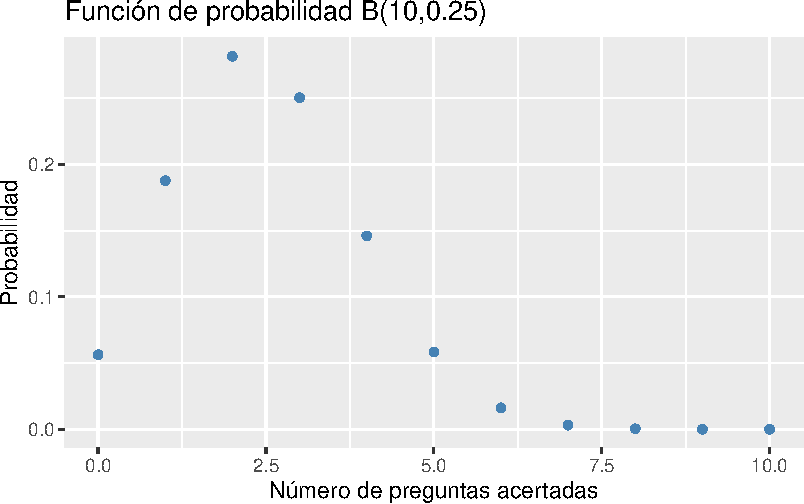
\includegraphics{./03-frecuencias-graficos_files/figure-pdf/unnamed-chunk-5-1.pdf}

}

\end{figure}

\begin{Shaded}
\begin{Highlighting}[]
\CommentTok{\# Diagrama de barras de frecuencias relativas.}
\FunctionTok{barplot}\NormalTok{(fi, }\AttributeTok{col =} \StringTok{"steelblue"}\NormalTok{, }\AttributeTok{main=}\StringTok{"Distribución del número de hijos"}\NormalTok{, }\AttributeTok{xlab=}\StringTok{"Hijos"}\NormalTok{, }\AttributeTok{ylab=}\StringTok{"Frecuencia relativa"}\NormalTok{)}
\end{Highlighting}
\end{Shaded}

\begin{figure}[H]

{\centering 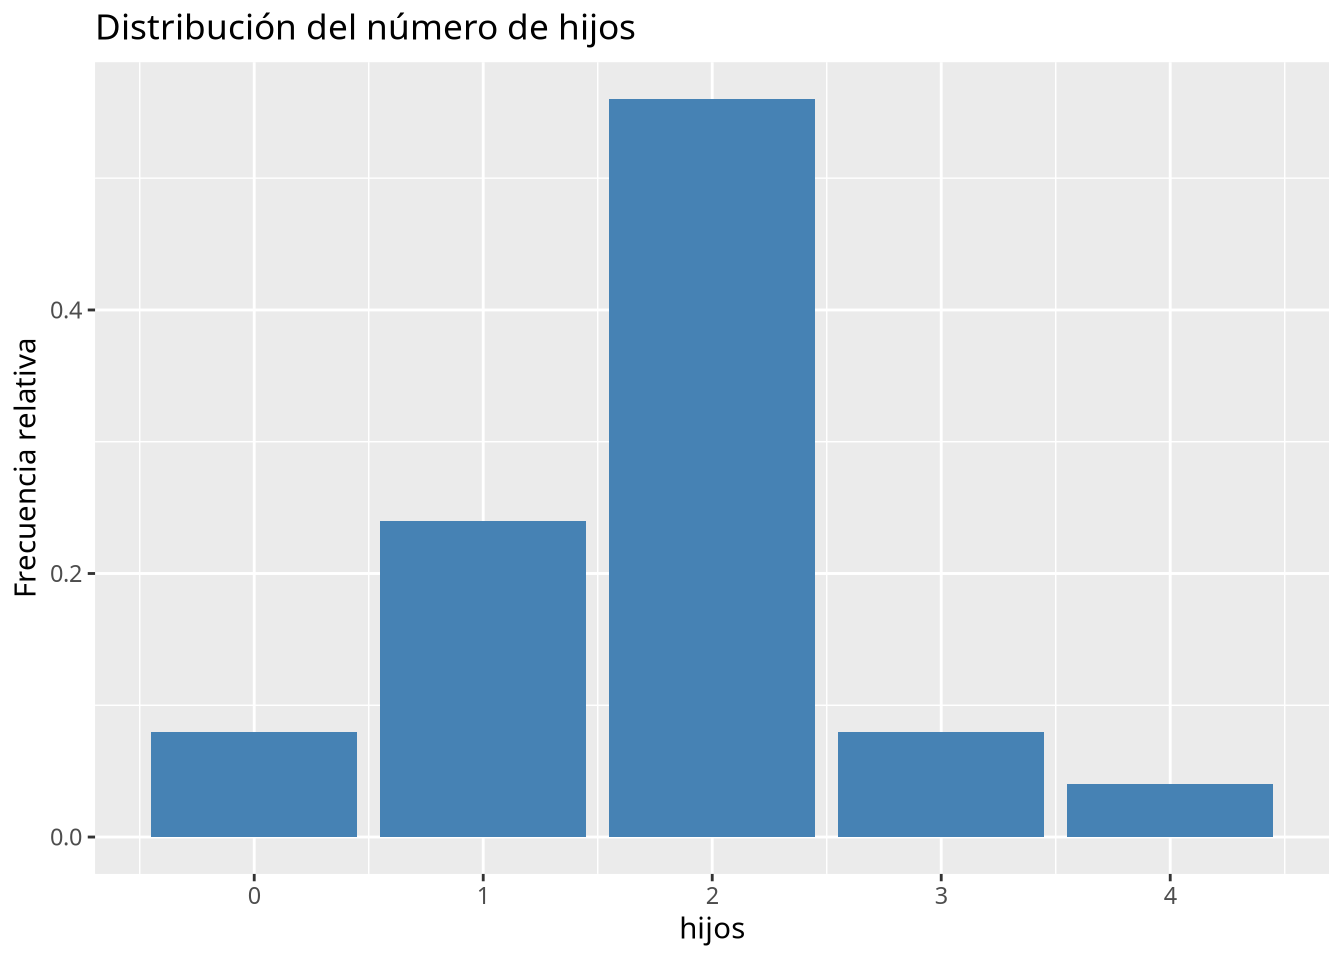
\includegraphics{./03-frecuencias-graficos_files/figure-pdf/unnamed-chunk-5-2.pdf}

}

\end{figure}

\begin{Shaded}
\begin{Highlighting}[]
\CommentTok{\# Diagrama de barras de frecuencias absolutas acumuladas.}
\FunctionTok{barplot}\NormalTok{(Ni, }\AttributeTok{col =} \StringTok{"steelblue"}\NormalTok{, }\AttributeTok{main=}\StringTok{"Distribución acumulada del número de hijos"}\NormalTok{, }\AttributeTok{xlab=}\StringTok{"Hijos"}\NormalTok{, }\AttributeTok{ylab=}\StringTok{"Frecuencia absoluta acumulada"}\NormalTok{)}
\end{Highlighting}
\end{Shaded}

\begin{figure}[H]

{\centering 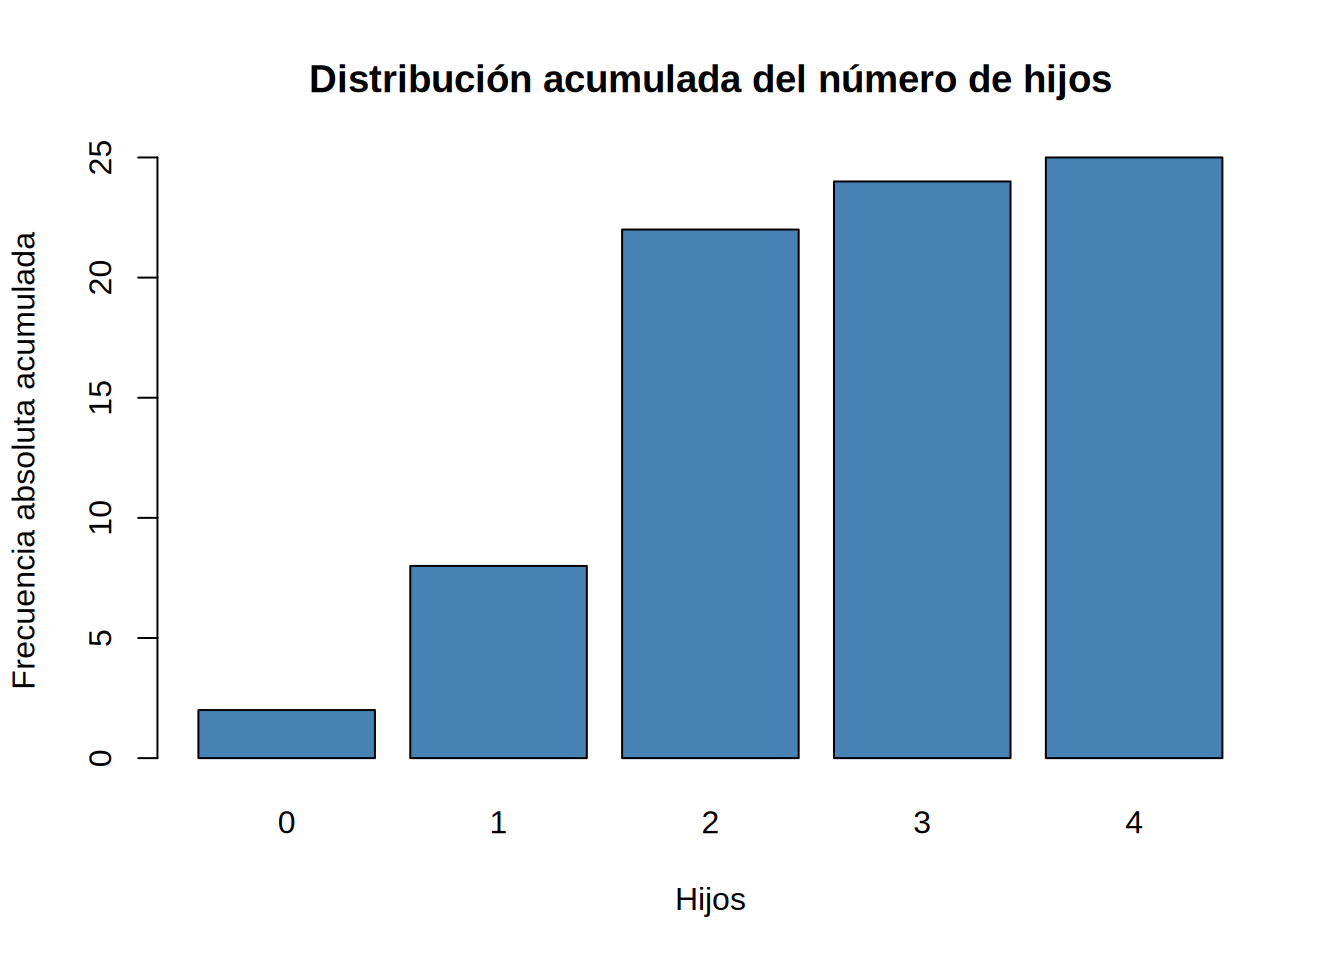
\includegraphics{./03-frecuencias-graficos_files/figure-pdf/unnamed-chunk-5-3.pdf}

}

\end{figure}

\begin{Shaded}
\begin{Highlighting}[]
\CommentTok{\# Diagrama de barras de frecuencias relativas acumuladas.}
\FunctionTok{barplot}\NormalTok{(Fi, }\AttributeTok{col =} \StringTok{"steelblue"}\NormalTok{, }\AttributeTok{main=}\StringTok{"Distribución acumulada del número de hijos"}\NormalTok{, }\AttributeTok{xlab=}\StringTok{"Hijos"}\NormalTok{, }\AttributeTok{ylab=}\StringTok{"Frecuencia relativa acumulada"}\NormalTok{)}
\end{Highlighting}
\end{Shaded}

\begin{figure}[H]

{\centering 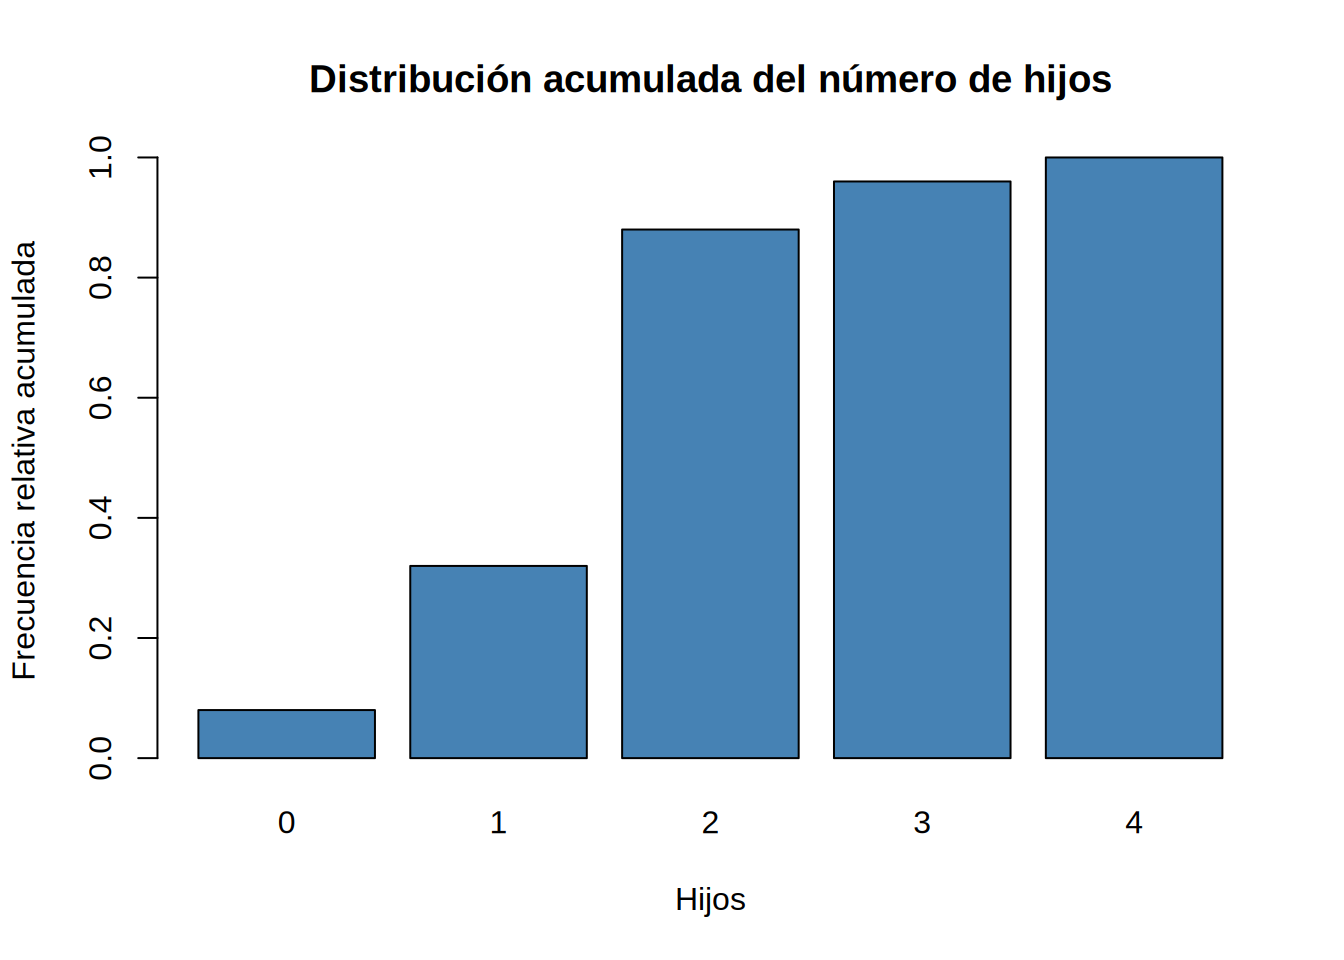
\includegraphics{./03-frecuencias-graficos_files/figure-pdf/unnamed-chunk-5-4.pdf}

}

\end{figure}

\end{tcolorbox}

\begin{tcolorbox}[enhanced jigsaw, rightrule=.15mm, toptitle=1mm, colbacktitle=quarto-callout-tip-color!10!white, titlerule=0mm, colback=white, leftrule=.75mm, bottomtitle=1mm, colframe=quarto-callout-tip-color-frame, breakable, title=\textcolor{quarto-callout-tip-color}{\faLightbulb}\hspace{0.5em}{Solución 2}, arc=.35mm, coltitle=black, opacityback=0, bottomrule=.15mm, opacitybacktitle=0.6, left=2mm, toprule=.15mm]

Otra alternativa es usar la función la función
\href{https://aprendeconalf.es/manual-r/07-graficos.html\#diagramas-de-barras}{\texttt{geom\_bar}}
del paquete \texttt{ggplot2}.

\begin{Shaded}
\begin{Highlighting}[]
\FunctionTok{library}\NormalTok{(ggplot2)}
\CommentTok{\# Diagarma de barras de frecuencias absolutas}
\FunctionTok{ggplot}\NormalTok{(df, }\FunctionTok{aes}\NormalTok{(}\AttributeTok{x =}\NormalTok{ hijos)) }\SpecialCharTok{+}
    \FunctionTok{geom\_bar}\NormalTok{(}\AttributeTok{fill =} \StringTok{"steelblue"}\NormalTok{) }\SpecialCharTok{+} 
    \FunctionTok{labs}\NormalTok{(}\AttributeTok{title =} \StringTok{"Distribución del número de hijos"}\NormalTok{, }\AttributeTok{y =} \StringTok{"Frecuencia absoluta"}\NormalTok{)}
\end{Highlighting}
\end{Shaded}

\begin{figure}[H]

{\centering 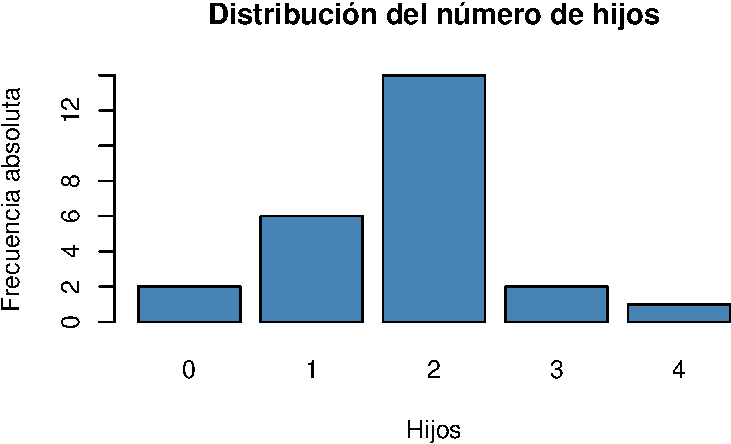
\includegraphics{./03-frecuencias-graficos_files/figure-pdf/unnamed-chunk-6-1.pdf}

}

\end{figure}

\begin{Shaded}
\begin{Highlighting}[]
\CommentTok{\# Diagarma de barras de frecuencias relativas}
\FunctionTok{ggplot}\NormalTok{(df, }\FunctionTok{aes}\NormalTok{(}\AttributeTok{x =}\NormalTok{ hijos)) }\SpecialCharTok{+}
    \FunctionTok{geom\_bar}\NormalTok{(}\FunctionTok{aes}\NormalTok{(}\AttributeTok{y =}\NormalTok{ (..count..)}\SpecialCharTok{/}\FunctionTok{sum}\NormalTok{(..count..)), }\AttributeTok{fill =} \StringTok{"steelblue"}\NormalTok{) }\SpecialCharTok{+}
    \FunctionTok{labs}\NormalTok{(}\AttributeTok{title =} \StringTok{"Distribución del número de hijos"}\NormalTok{, }\AttributeTok{y =} \StringTok{"Frecuencia relativa"}\NormalTok{)}
\end{Highlighting}
\end{Shaded}

\begin{figure}[H]

{\centering 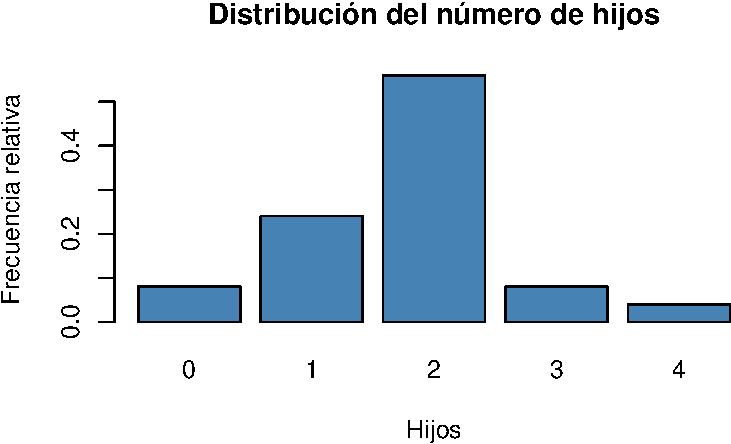
\includegraphics{./03-frecuencias-graficos_files/figure-pdf/unnamed-chunk-6-2.pdf}

}

\end{figure}

\begin{Shaded}
\begin{Highlighting}[]
\CommentTok{\# Diagarma de barras de frecuencias acumuladas}
\FunctionTok{ggplot}\NormalTok{(df, }\FunctionTok{aes}\NormalTok{(}\AttributeTok{x =}\NormalTok{ hijos)) }\SpecialCharTok{+}
    \FunctionTok{geom\_bar}\NormalTok{(}\FunctionTok{aes}\NormalTok{(}\AttributeTok{y =} \FunctionTok{cumsum}\NormalTok{(..count..)), }\AttributeTok{fill =} \StringTok{"steelblue"}\NormalTok{) }\SpecialCharTok{+}
    \FunctionTok{labs}\NormalTok{(}\AttributeTok{title =} \StringTok{"Distribución acumulada del número de hijos"}\NormalTok{, }\AttributeTok{y =} \StringTok{"Frecuencia absoluta acumulada"}\NormalTok{)}
\end{Highlighting}
\end{Shaded}

\begin{figure}[H]

{\centering 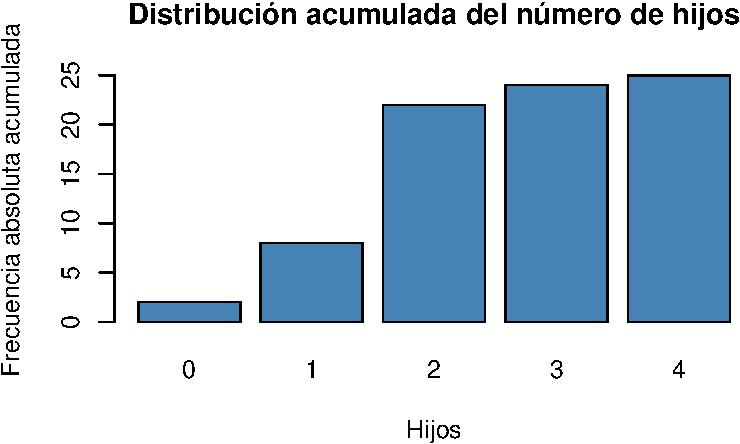
\includegraphics{./03-frecuencias-graficos_files/figure-pdf/unnamed-chunk-6-3.pdf}

}

\end{figure}

\begin{Shaded}
\begin{Highlighting}[]
\CommentTok{\# Diagarma de barras de frecuencias acumuladas}
\FunctionTok{ggplot}\NormalTok{(df, }\FunctionTok{aes}\NormalTok{(}\AttributeTok{x =}\NormalTok{ hijos)) }\SpecialCharTok{+}
    \FunctionTok{geom\_bar}\NormalTok{(}\FunctionTok{aes}\NormalTok{(}\AttributeTok{y =} \FunctionTok{cumsum}\NormalTok{(..count..)}\SpecialCharTok{/}\FunctionTok{sum}\NormalTok{(..count..)), }\AttributeTok{fill =} \StringTok{"steelblue"}\NormalTok{) }\SpecialCharTok{+}
    \FunctionTok{labs}\NormalTok{(}\AttributeTok{title =} \StringTok{"Distribución acumulada del número de hijos"}\NormalTok{, }\AttributeTok{y =} \StringTok{"Frecuencia relativa acumulada"}\NormalTok{)}
\end{Highlighting}
\end{Shaded}

\begin{figure}[H]

{\centering 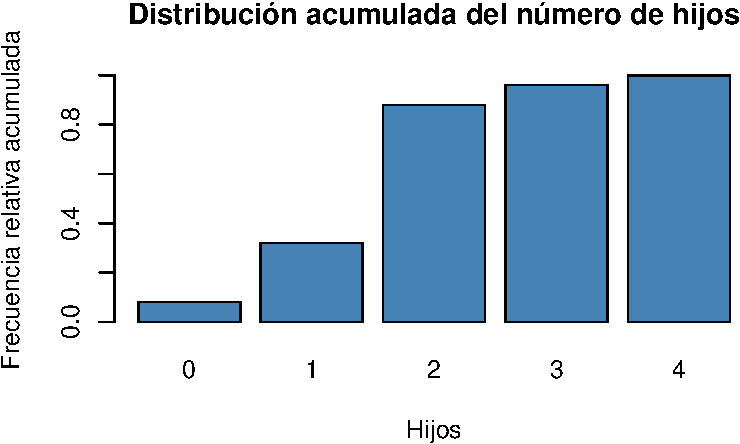
\includegraphics{./03-frecuencias-graficos_files/figure-pdf/unnamed-chunk-6-4.pdf}

}

\end{figure}

\end{tcolorbox}

\begin{enumerate}
\def\labelenumi{\alph{enumi}.}
\setcounter{enumi}{3}
\tightlist
\item
  Dibujar el polígono de frecuencias relativas.
\end{enumerate}

\begin{tcolorbox}[enhanced jigsaw, rightrule=.15mm, toptitle=1mm, colbacktitle=quarto-callout-tip-color!10!white, titlerule=0mm, colback=white, leftrule=.75mm, bottomtitle=1mm, colframe=quarto-callout-tip-color-frame, breakable, title=\textcolor{quarto-callout-tip-color}{\faLightbulb}\hspace{0.5em}{Solución 1}, arc=.35mm, coltitle=black, opacityback=0, bottomrule=.15mm, opacitybacktitle=0.6, left=2mm, toprule=.15mm]

Para dibujar un diagrama de lineas se puede usar la función
\href{https://www.rdocumentation.org/packages/graphics/versions/3.6.2/topics/plot}{\texttt{plot}}
del paquete \texttt{graphics}.

\begin{Shaded}
\begin{Highlighting}[]
\CommentTok{\# Frecuencias relativas.}
\FunctionTok{plot}\NormalTok{(}\FunctionTok{names}\NormalTok{(fi), fi, }\AttributeTok{type =} \StringTok{"l"}\NormalTok{, }\AttributeTok{col =} \StringTok{"steelblue"}\NormalTok{, }\AttributeTok{main=}\StringTok{"Distribución del número de hijos"}\NormalTok{, }\AttributeTok{xlab=}\StringTok{"Hijos"}\NormalTok{, }\AttributeTok{ylab=}\StringTok{"Frecuencia relativa"}\NormalTok{)}
\end{Highlighting}
\end{Shaded}

\begin{figure}[H]

{\centering 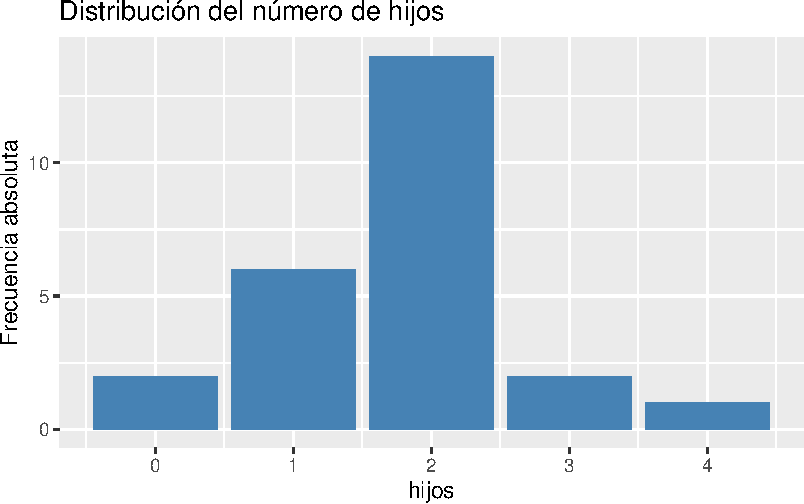
\includegraphics{./03-frecuencias-graficos_files/figure-pdf/unnamed-chunk-7-1.pdf}

}

\end{figure}

\end{tcolorbox}

\begin{tcolorbox}[enhanced jigsaw, rightrule=.15mm, toptitle=1mm, colbacktitle=quarto-callout-tip-color!10!white, titlerule=0mm, colback=white, leftrule=.75mm, bottomtitle=1mm, colframe=quarto-callout-tip-color-frame, breakable, title=\textcolor{quarto-callout-tip-color}{\faLightbulb}\hspace{0.5em}{Solución 2}, arc=.35mm, coltitle=black, opacityback=0, bottomrule=.15mm, opacitybacktitle=0.6, left=2mm, toprule=.15mm]

Otra alternativa es usar la función la función
\href{https://aprendeconalf.es/manual-r/07-graficos.html\#diagramas-de-lineas}{\texttt{geom\_line}}
del paquete \texttt{ggplot2}.

\begin{Shaded}
\begin{Highlighting}[]
\FunctionTok{library}\NormalTok{(ggplot2)}
\FunctionTok{count}\NormalTok{(df, hijos) }\SpecialCharTok{\%\textgreater{}\%} 
    \FunctionTok{mutate}\NormalTok{(}\AttributeTok{fi =}\NormalTok{ n}\SpecialCharTok{/}\FunctionTok{sum}\NormalTok{(n)) }\SpecialCharTok{\%\textgreater{}\%}
    \FunctionTok{ggplot}\NormalTok{(}\FunctionTok{aes}\NormalTok{(}\AttributeTok{x=}\NormalTok{hijos, }\AttributeTok{y=}\NormalTok{fi)) }\SpecialCharTok{+}
    \FunctionTok{geom\_line}\NormalTok{(}\AttributeTok{col =} \StringTok{"steelblue"}\NormalTok{) }\SpecialCharTok{+}
    \FunctionTok{labs}\NormalTok{(}\AttributeTok{title =} \StringTok{"Distribución del número de hijos"}\NormalTok{, }\AttributeTok{y =} \StringTok{"Frecuencia relativa"}\NormalTok{)}
\end{Highlighting}
\end{Shaded}

\begin{figure}[H]

{\centering 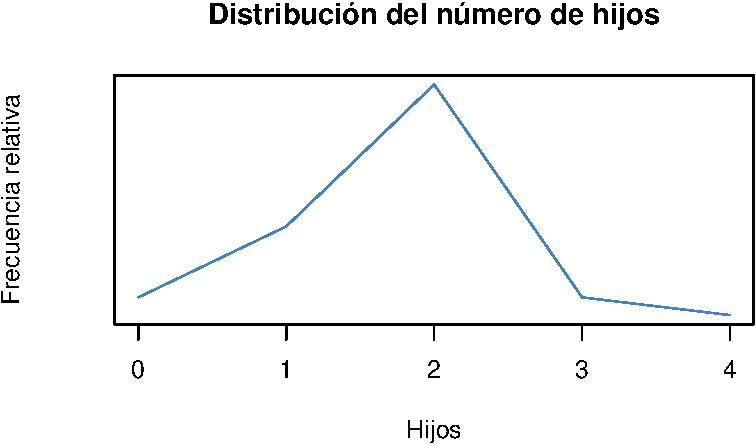
\includegraphics{./03-frecuencias-graficos_files/figure-pdf/unnamed-chunk-8-1.pdf}

}

\end{figure}

\end{tcolorbox}

\end{exercise}

\leavevmode\vadjust pre{\hypertarget{exr-2}{}}%
\begin{exercise}[]\label{exr-2}

En un servicio de atención al cliente se han registrado el número de
llamadas de clientes cada día del mes de noviembre, obteniendo los
siguientes datos:

\begin{longtable}[]{@{}
  >{\centering\arraybackslash}p{(\columnwidth - 0\tabcolsep) * \real{1.0000}}@{}}
\toprule()
\endhead
15, 23, 12, 10, 28, 50, 12, 17, 20, 21, 18, 13, 11, 12, 26, 30, 6, 16,
19, 22, 14, 17, 21, 28, 9, 16, 13, 11, 16, 20 \\
\bottomrule()
\end{longtable}

\begin{enumerate}
\def\labelenumi{\alph{enumi}.}
\tightlist
\item
  Crear un conjunto de datos con la variable \texttt{llamadas}.
\end{enumerate}

\begin{tcolorbox}[enhanced jigsaw, rightrule=.15mm, toptitle=1mm, colbacktitle=quarto-callout-tip-color!10!white, titlerule=0mm, colback=white, leftrule=.75mm, bottomtitle=1mm, colframe=quarto-callout-tip-color-frame, breakable, title=\textcolor{quarto-callout-tip-color}{\faLightbulb}\hspace{0.5em}{Solución}, arc=.35mm, coltitle=black, opacityback=0, bottomrule=.15mm, opacitybacktitle=0.6, left=2mm, toprule=.15mm]

\begin{Shaded}
\begin{Highlighting}[]
\NormalTok{df }\OtherTok{\textless{}{-}} \FunctionTok{data.frame}\NormalTok{(}\AttributeTok{llamadas =} \FunctionTok{c}\NormalTok{(}\DecValTok{15}\NormalTok{, }\DecValTok{23}\NormalTok{, }\DecValTok{12}\NormalTok{, }\DecValTok{10}\NormalTok{, }\DecValTok{28}\NormalTok{, }\DecValTok{50}\NormalTok{, }\DecValTok{12}\NormalTok{, }\DecValTok{17}\NormalTok{, }\DecValTok{20}\NormalTok{, }\DecValTok{21}\NormalTok{, }\DecValTok{18}\NormalTok{, }\DecValTok{13}\NormalTok{, }\DecValTok{11}\NormalTok{, }\DecValTok{12}\NormalTok{, }\DecValTok{26}\NormalTok{, }\DecValTok{30}\NormalTok{, }\DecValTok{6}\NormalTok{, }\DecValTok{16}\NormalTok{, }\DecValTok{19}\NormalTok{, }\DecValTok{22}\NormalTok{, }\DecValTok{14}\NormalTok{, }\DecValTok{17}\NormalTok{, }\DecValTok{21}\NormalTok{, }\DecValTok{28}\NormalTok{, }\DecValTok{9}\NormalTok{, }\DecValTok{16}\NormalTok{, }\DecValTok{13}\NormalTok{, }\DecValTok{11}\NormalTok{, }\DecValTok{16}\NormalTok{, }\DecValTok{20}\NormalTok{))}
\end{Highlighting}
\end{Shaded}

\end{tcolorbox}

\begin{enumerate}
\def\labelenumi{\alph{enumi}.}
\setcounter{enumi}{1}
\tightlist
\item
  Dibujar el diagrama de cajas. ¿Existe algún dato atípico? En el caso
  de que exista, eliminarlo y proceder con los siguientes apartados.
\end{enumerate}

\begin{tcolorbox}[enhanced jigsaw, rightrule=.15mm, toptitle=1mm, colbacktitle=quarto-callout-tip-color!10!white, titlerule=0mm, colback=white, leftrule=.75mm, bottomtitle=1mm, colframe=quarto-callout-tip-color-frame, breakable, title=\textcolor{quarto-callout-tip-color}{\faLightbulb}\hspace{0.5em}{Solución 1}, arc=.35mm, coltitle=black, opacityback=0, bottomrule=.15mm, opacitybacktitle=0.6, left=2mm, toprule=.15mm]

Para dibujar un diagrama de cajas se puede usar la función
\href{https://www.rdocumentation.org/packages/graphics/versions/3.6.2/topics/boxplot}{\texttt{boxplot}}
del paquete \texttt{graphics}.

\begin{Shaded}
\begin{Highlighting}[]
\CommentTok{\# Frecuencias relativas.}
\FunctionTok{boxplot}\NormalTok{(df}\SpecialCharTok{$}\NormalTok{llamadas, }\AttributeTok{col =} \StringTok{"steelblue"}\NormalTok{, }\AttributeTok{main=}\StringTok{"Distribución del número de llamadas"}\NormalTok{, }\AttributeTok{horizontal =}\NormalTok{ T, }\AttributeTok{xlab=}\StringTok{"Número de llamadas"}\NormalTok{)}
\end{Highlighting}
\end{Shaded}

\begin{figure}[H]

{\centering 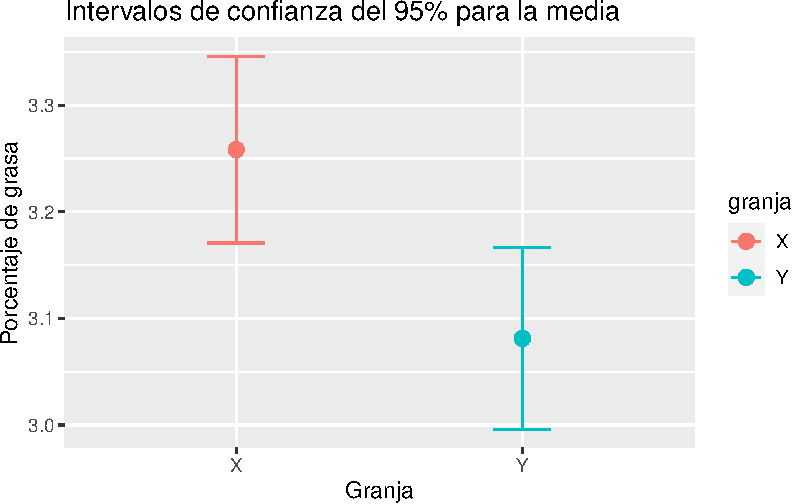
\includegraphics{./03-frecuencias-graficos_files/figure-pdf/unnamed-chunk-10-1.pdf}

}

\end{figure}

\end{tcolorbox}

\begin{tcolorbox}[enhanced jigsaw, rightrule=.15mm, toptitle=1mm, colbacktitle=quarto-callout-tip-color!10!white, titlerule=0mm, colback=white, leftrule=.75mm, bottomtitle=1mm, colframe=quarto-callout-tip-color-frame, breakable, title=\textcolor{quarto-callout-tip-color}{\faLightbulb}\hspace{0.5em}{Solución 2}, arc=.35mm, coltitle=black, opacityback=0, bottomrule=.15mm, opacitybacktitle=0.6, left=2mm, toprule=.15mm]

Otra alternativa es usar la función la función
\href{https://aprendeconalf.es/manual-r/07-graficos.html\#diagramas-de-cajas}{\texttt{geom\_boxplot}}
del paquete \texttt{ggplot2}.

\begin{Shaded}
\begin{Highlighting}[]
\FunctionTok{library}\NormalTok{(ggplot2)}
\FunctionTok{ggplot}\NormalTok{(df, }\FunctionTok{aes}\NormalTok{(}\AttributeTok{x =}\NormalTok{ llamadas)) }\SpecialCharTok{+}
    \FunctionTok{geom\_boxplot}\NormalTok{(}\AttributeTok{fill =} \StringTok{"steelblue"}\NormalTok{) }\SpecialCharTok{+}
    \FunctionTok{labs}\NormalTok{(}\AttributeTok{title =} \StringTok{"Distribución del número de llamadas"}\NormalTok{, }\AttributeTok{x =} \StringTok{"Número de llamadas"}\NormalTok{)}
\end{Highlighting}
\end{Shaded}

\begin{figure}[H]

{\centering 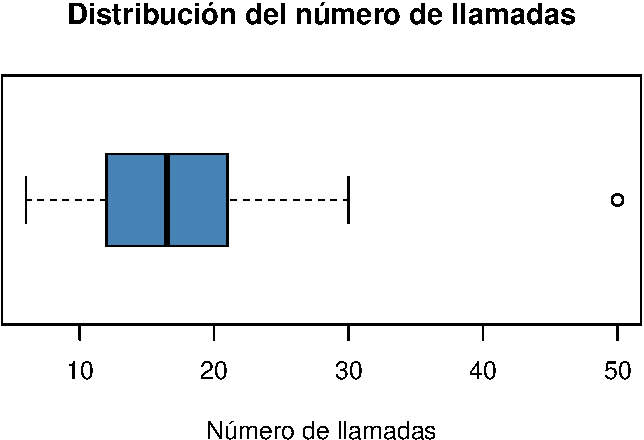
\includegraphics{./03-frecuencias-graficos_files/figure-pdf/unnamed-chunk-11-1.pdf}

}

\end{figure}

Hay un día con 50 llamadas, que es un valor atípico en comparación con
el resto de días.

\begin{tcolorbox}[enhanced jigsaw, rightrule=.15mm, toptitle=1mm, colbacktitle=quarto-callout-tip-color!10!white, titlerule=0mm, colback=white, leftrule=.75mm, bottomtitle=1mm, colframe=quarto-callout-tip-color-frame, breakable, title=\textcolor{quarto-callout-tip-color}{\faLightbulb}\hspace{0.5em}{Solución}, arc=.35mm, coltitle=black, opacityback=0, bottomrule=.15mm, opacitybacktitle=0.6, left=2mm, toprule=.15mm]

La función \texttt{cut}

\begin{Shaded}
\begin{Highlighting}[]
\CommentTok{\# Eliminación del dato atípico.}
\NormalTok{df }\OtherTok{\textless{}{-}}\NormalTok{ df[df}\SpecialCharTok{$}\NormalTok{llamadas }\SpecialCharTok{!=} \DecValTok{50}\NormalTok{, , drop }\OtherTok{=}\NormalTok{ F]}
\end{Highlighting}
\end{Shaded}

\end{tcolorbox}

\end{tcolorbox}

\begin{enumerate}
\def\labelenumi{\alph{enumi}.}
\setcounter{enumi}{2}
\tightlist
\item
  Construir la tabla de frecuencias agrupando en 5 clases.
\end{enumerate}

\begin{tcolorbox}[enhanced jigsaw, rightrule=.15mm, toptitle=1mm, colbacktitle=quarto-callout-tip-color!10!white, titlerule=0mm, colback=white, leftrule=.75mm, bottomtitle=1mm, colframe=quarto-callout-tip-color-frame, breakable, title=\textcolor{quarto-callout-tip-color}{\faLightbulb}\hspace{0.5em}{Solución 1}, arc=.35mm, coltitle=black, opacityback=0, bottomrule=.15mm, opacitybacktitle=0.6, left=2mm, toprule=.15mm]

Para agrupar los datos en intervalos se puede utilizar la función
\href{https://www.rdocumentation.org/packages/base/versions/3.6.2/topics/cut}{\texttt{cut}}
del paquete base de R, y para contar las frecuencias absolutas y
relativas las funciones
\href{https://www.rdocumentation.org/packages/base/versions/3.6.2/topics/table}{\texttt{table}},
y
\href{https://www.rdocumentation.org/packages/base/versions/3.6.2/topics/prop.table}{\texttt{prop.table}}
respectivamente.

\begin{Shaded}
\begin{Highlighting}[]
\CommentTok{\# Frecuencias absolutas. Creación automática de 5 clases con intervalos cerrados a la izquierda.}
\end{Highlighting}
\end{Shaded}

\begin{Shaded}
\begin{Highlighting}[]
\NormalTok{ni }\OtherTok{\textless{}{-}} \FunctionTok{table}\NormalTok{(}\FunctionTok{cut}\NormalTok{(df}\SpecialCharTok{$}\NormalTok{llamadas, }\AttributeTok{breaks =} \DecValTok{5}\NormalTok{, }\AttributeTok{right =}\NormalTok{ F))}
\CommentTok{\# Creación manual de 5 clases.}
\NormalTok{ni }\OtherTok{\textless{}{-}} \FunctionTok{table}\NormalTok{(}\FunctionTok{cut}\NormalTok{(df}\SpecialCharTok{$}\NormalTok{llamadas, }\AttributeTok{breaks =} \FunctionTok{seq}\NormalTok{(}\DecValTok{5}\NormalTok{, }\DecValTok{30}\NormalTok{, }\DecValTok{5}\NormalTok{)))}
\CommentTok{\# Frecuencias relativas}
\NormalTok{fi }\OtherTok{\textless{}{-}} \FunctionTok{prop.table}\NormalTok{(ni)}
\CommentTok{\# Frecuencias acumuladas.}
\NormalTok{Ni }\OtherTok{\textless{}{-}} \FunctionTok{cumsum}\NormalTok{(ni)}
\CommentTok{\# Frecuencias relativas acumuladas.}
\NormalTok{Fi }\OtherTok{\textless{}{-}} \FunctionTok{cumsum}\NormalTok{(fi)}
\CommentTok{\# Creación de un data frame con las frecuencias.}
\NormalTok{tabla\_frec }\OtherTok{\textless{}{-}} \FunctionTok{cbind}\NormalTok{(ni, fi, Ni, Fi)}
\NormalTok{tabla\_frec}
\end{Highlighting}
\end{Shaded}

\begin{verbatim}
        ni        fi Ni        Fi
(5,10]   3 0.1034483  3 0.1034483
(10,15]  9 0.3103448 12 0.4137931
(15,20]  9 0.3103448 21 0.7241379
(20,25]  4 0.1379310 25 0.8620690
(25,30]  4 0.1379310 29 1.0000000
\end{verbatim}

\end{tcolorbox}

\begin{tcolorbox}[enhanced jigsaw, rightrule=.15mm, toptitle=1mm, colbacktitle=quarto-callout-tip-color!10!white, titlerule=0mm, colback=white, leftrule=.75mm, bottomtitle=1mm, colframe=quarto-callout-tip-color-frame, breakable, title=\textcolor{quarto-callout-tip-color}{\faLightbulb}\hspace{0.5em}{Solución 2}, arc=.35mm, coltitle=black, opacityback=0, bottomrule=.15mm, opacitybacktitle=0.6, left=2mm, toprule=.15mm]

Otra alternativa es usar la fución
\href{https://aprendeconalf.es/manual-r/06-preprocesamiento.html\#conteo-del-n\%C3\%BAmero-de-observaciones}{\texttt{count}}
del paquete \texttt{dplyr}.

\begin{Shaded}
\begin{Highlighting}[]
\FunctionTok{library}\NormalTok{(dplyr)}
\FunctionTok{library}\NormalTok{(knitr)}
\FunctionTok{library}\NormalTok{(kableExtra)}
\FunctionTok{mutate}\NormalTok{(df, }\AttributeTok{llamadas\_int =} \FunctionTok{cut}\NormalTok{(llamadas, }\AttributeTok{breaks =} \FunctionTok{seq}\NormalTok{(}\DecValTok{5}\NormalTok{, }\DecValTok{30}\NormalTok{, }\DecValTok{5}\NormalTok{))) }\SpecialCharTok{\%\textgreater{}\%} 
    \FunctionTok{count}\NormalTok{(llamadas\_int) }\SpecialCharTok{\%\textgreater{}\%}
    \FunctionTok{mutate}\NormalTok{(}\AttributeTok{fi =}\NormalTok{ n}\SpecialCharTok{/}\FunctionTok{sum}\NormalTok{(n), }\AttributeTok{Ni =} \FunctionTok{cumsum}\NormalTok{(n), }\AttributeTok{Fi =} \FunctionTok{cumsum}\NormalTok{(n)}\SpecialCharTok{/}\FunctionTok{sum}\NormalTok{(n)) }\SpecialCharTok{\%\textgreater{}\%}
    \FunctionTok{kable}\NormalTok{() }
\end{Highlighting}
\end{Shaded}

\begin{tabular}{l|r|r|r|r}
\hline
llamadas\_int & n & fi & Ni & Fi\\
\hline
(5,10] & 3 & 0.1034483 & 3 & 0.1034483\\
\hline
(10,15] & 9 & 0.3103448 & 12 & 0.4137931\\
\hline
(15,20] & 9 & 0.3103448 & 21 & 0.7241379\\
\hline
(20,25] & 4 & 0.1379310 & 25 & 0.8620690\\
\hline
(25,30] & 4 & 0.1379310 & 29 & 1.0000000\\
\hline
\end{tabular}

\begin{Shaded}
\begin{Highlighting}[]
    \CommentTok{\#\%\textgreater{}\%}
    \CommentTok{\#kable\_styling(bootstrap\_options = "hover", full\_width = F)}
\end{Highlighting}
\end{Shaded}

\end{tcolorbox}

\begin{enumerate}
\def\labelenumi{\alph{enumi}.}
\setcounter{enumi}{3}
\tightlist
\item
  Dibujar el histograma de frecuencias absolutas, relativas, absolutas
  acumuladas y relativas acumuladas correspondiente a la tabla anterior.
\end{enumerate}

\begin{tcolorbox}[enhanced jigsaw, rightrule=.15mm, toptitle=1mm, colbacktitle=quarto-callout-tip-color!10!white, titlerule=0mm, colback=white, leftrule=.75mm, bottomtitle=1mm, colframe=quarto-callout-tip-color-frame, breakable, title=\textcolor{quarto-callout-tip-color}{\faLightbulb}\hspace{0.5em}{Solución 1}, arc=.35mm, coltitle=black, opacityback=0, bottomrule=.15mm, opacitybacktitle=0.6, left=2mm, toprule=.15mm]

Para dibujar un histograma se puede usar la función
\href{https://www.rdocumentation.org/packages/graphics/versions/3.6.2/topics/hist}{\texttt{hist}}
del paquete \texttt{graphics}.

\begin{Shaded}
\begin{Highlighting}[]
\CommentTok{\# Histograma de frecuencias absolutas.}
\NormalTok{histo }\OtherTok{\textless{}{-}} \FunctionTok{hist}\NormalTok{(df}\SpecialCharTok{$}\NormalTok{llamadas, }\AttributeTok{breaks =} \FunctionTok{seq}\NormalTok{(}\DecValTok{5}\NormalTok{, }\DecValTok{30}\NormalTok{, }\DecValTok{5}\NormalTok{), }\AttributeTok{col =} \StringTok{"steelblue"}\NormalTok{, }\AttributeTok{main=}\StringTok{"Distribución del número de llamadas"}\NormalTok{, }\AttributeTok{xlab=}\StringTok{"Llamadas"}\NormalTok{, }\AttributeTok{ylab=}\StringTok{"Frecuencia absoluta"}\NormalTok{)}
\end{Highlighting}
\end{Shaded}

\begin{figure}[H]

{\centering 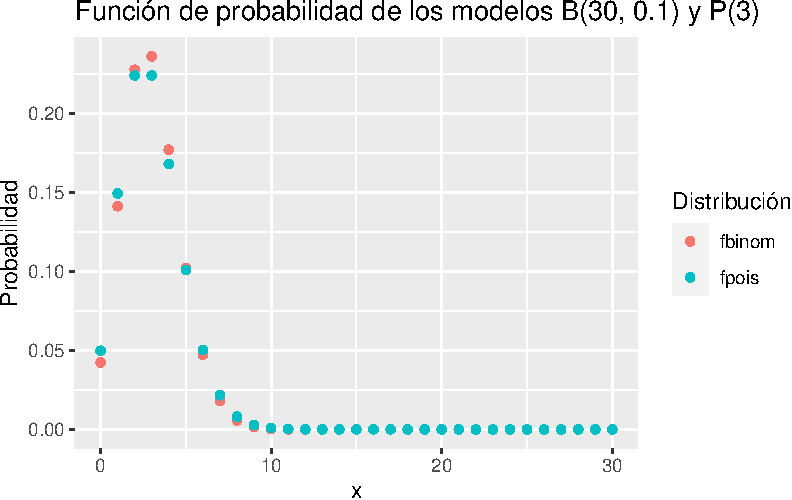
\includegraphics{./03-frecuencias-graficos_files/figure-pdf/unnamed-chunk-16-1.pdf}

}

\end{figure}

\begin{Shaded}
\begin{Highlighting}[]
\NormalTok{ni }\OtherTok{\textless{}{-}}\NormalTok{ histo}\SpecialCharTok{$}\NormalTok{counts}
\CommentTok{\# Histograma de frecuencias relativas.}
\NormalTok{histo}\SpecialCharTok{$}\NormalTok{counts }\OtherTok{\textless{}{-}}\NormalTok{ ni}\SpecialCharTok{/}\FunctionTok{sum}\NormalTok{(ni)}
\FunctionTok{plot}\NormalTok{(histo, }\AttributeTok{col =} \StringTok{"steelblue"}\NormalTok{, }\AttributeTok{main=}\StringTok{"Distribución del número de llamadas"}\NormalTok{, }\AttributeTok{xlab=}\StringTok{"Llamadas"}\NormalTok{, }\AttributeTok{ylab=}\StringTok{"Frecuencia relativa"}\NormalTok{)}
\end{Highlighting}
\end{Shaded}

\begin{figure}[H]

{\centering 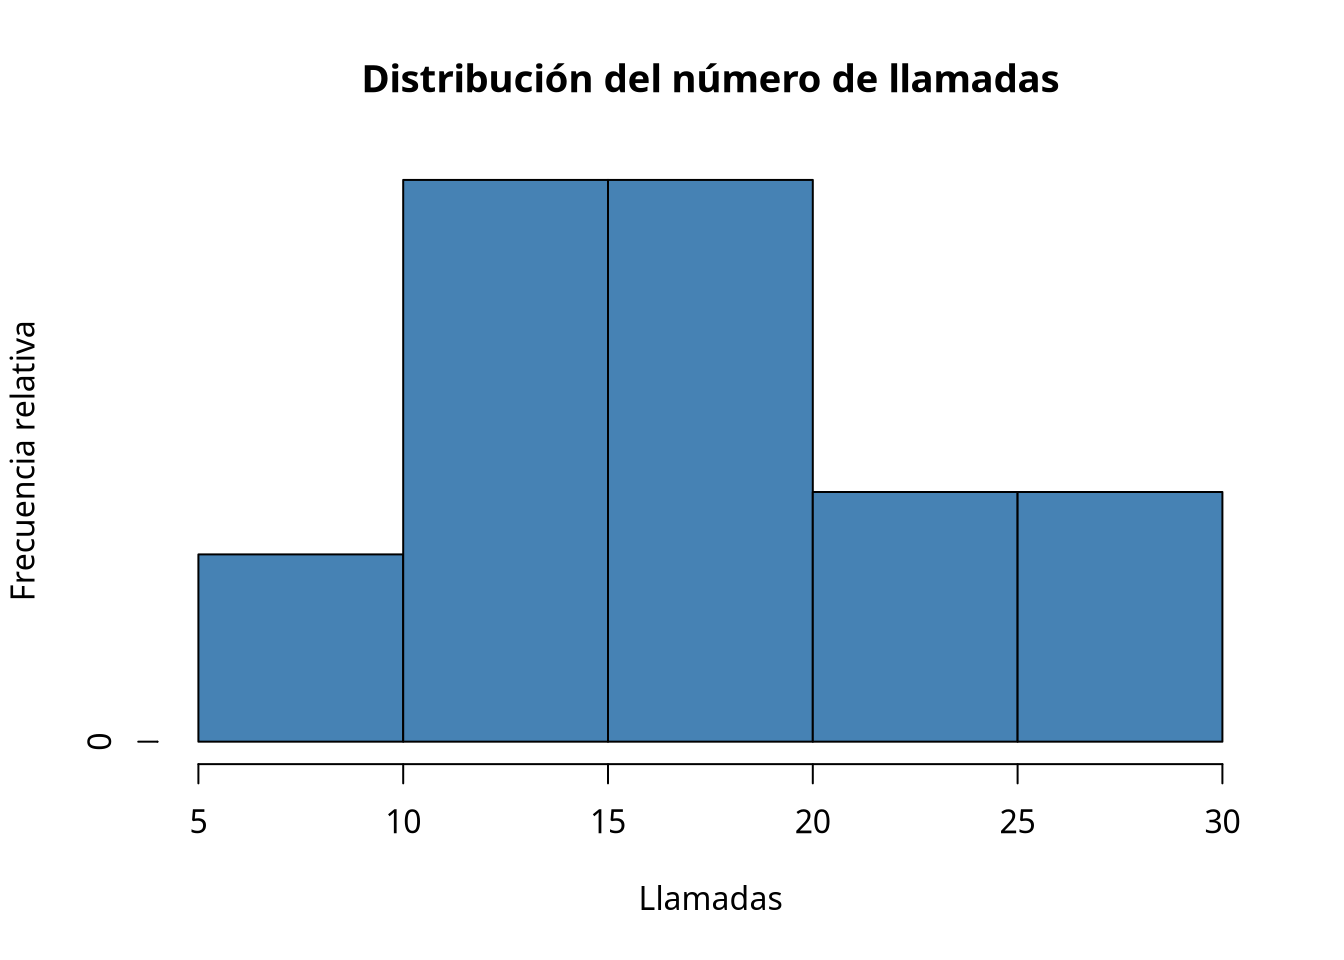
\includegraphics{./03-frecuencias-graficos_files/figure-pdf/unnamed-chunk-16-2.pdf}

}

\end{figure}

\begin{Shaded}
\begin{Highlighting}[]
\CommentTok{\# Histograma de frecuencias absolutas acumuladas.}
\NormalTok{histo}\SpecialCharTok{$}\NormalTok{counts }\OtherTok{\textless{}{-}} \FunctionTok{cumsum}\NormalTok{(ni)}
\FunctionTok{plot}\NormalTok{(histo, }\AttributeTok{col =} \StringTok{"steelblue"}\NormalTok{, }\AttributeTok{main=}\StringTok{"Distribución acumulada del número de llamadas"}\NormalTok{, }\AttributeTok{xlab=}\StringTok{"Llamadas"}\NormalTok{, }\AttributeTok{ylab=}\StringTok{"Frecuencia absoluta acumulada"}\NormalTok{)}
\end{Highlighting}
\end{Shaded}

\begin{figure}[H]

{\centering 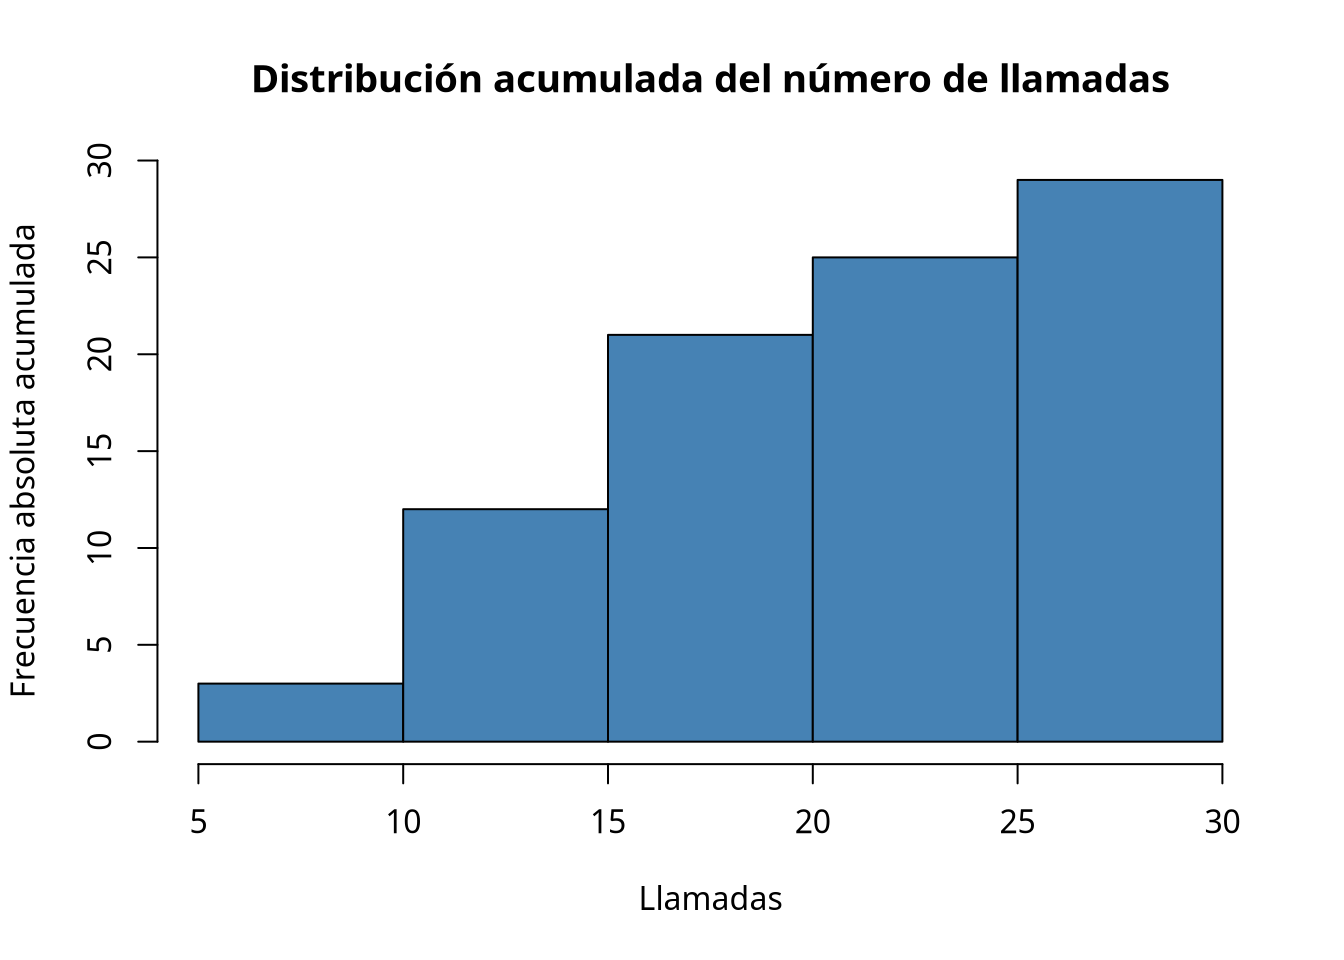
\includegraphics{./03-frecuencias-graficos_files/figure-pdf/unnamed-chunk-16-3.pdf}

}

\end{figure}

\begin{Shaded}
\begin{Highlighting}[]
\CommentTok{\# Histograma de frecuencias relativas acumuladas.}
\NormalTok{histo}\SpecialCharTok{$}\NormalTok{counts }\OtherTok{\textless{}{-}} \FunctionTok{cumsum}\NormalTok{(ni)}\SpecialCharTok{/}\FunctionTok{sum}\NormalTok{(ni)}
\FunctionTok{plot}\NormalTok{(histo, }\AttributeTok{col =} \StringTok{"steelblue"}\NormalTok{, }\AttributeTok{main=}\StringTok{"Distribución acumulada del número de llamadas"}\NormalTok{, }\AttributeTok{xlab=}\StringTok{"Llamadas"}\NormalTok{, }\AttributeTok{ylab=}\StringTok{"Frecuencia relativa acumulada"}\NormalTok{, )}
\end{Highlighting}
\end{Shaded}

\begin{figure}[H]

{\centering 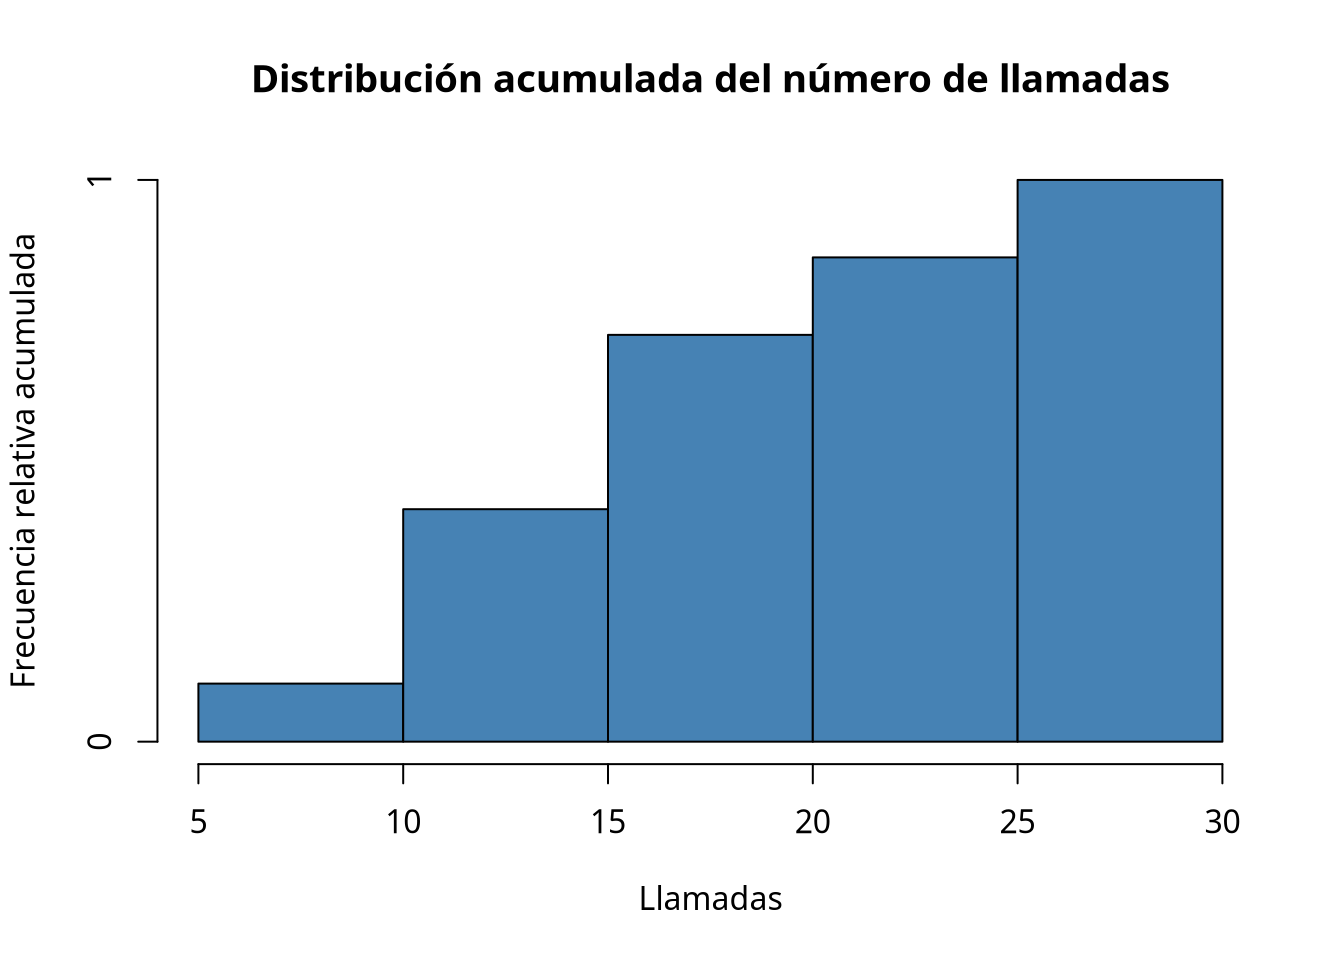
\includegraphics{./03-frecuencias-graficos_files/figure-pdf/unnamed-chunk-16-4.pdf}

}

\end{figure}

\end{tcolorbox}

\begin{tcolorbox}[enhanced jigsaw, rightrule=.15mm, toptitle=1mm, colbacktitle=quarto-callout-tip-color!10!white, titlerule=0mm, colback=white, leftrule=.75mm, bottomtitle=1mm, colframe=quarto-callout-tip-color-frame, breakable, title=\textcolor{quarto-callout-tip-color}{\faLightbulb}\hspace{0.5em}{Solución 2}, arc=.35mm, coltitle=black, opacityback=0, bottomrule=.15mm, opacitybacktitle=0.6, left=2mm, toprule=.15mm]

Otra alternativa es usar la función la función
\href{https://aprendeconalf.es/manual-r/07-graficos.html\#histogramas}{\texttt{geom\_histogram}}
del paquete \texttt{ggplot2}.

\begin{Shaded}
\begin{Highlighting}[]
\FunctionTok{library}\NormalTok{(ggplot2)}
\CommentTok{\# Histograma de frecuencias absolutas}
\FunctionTok{ggplot}\NormalTok{(df, }\FunctionTok{aes}\NormalTok{(}\AttributeTok{x =}\NormalTok{ llamadas)) }\SpecialCharTok{+}
    \FunctionTok{geom\_histogram}\NormalTok{(}\AttributeTok{breaks =} \FunctionTok{seq}\NormalTok{(}\DecValTok{5}\NormalTok{, }\DecValTok{30}\NormalTok{, }\DecValTok{5}\NormalTok{), }\AttributeTok{fill =} \StringTok{"steelblue"}\NormalTok{, }\AttributeTok{col =} \StringTok{"white"}\NormalTok{) }\SpecialCharTok{+} 
    \FunctionTok{labs}\NormalTok{(}\AttributeTok{title =} \StringTok{"Distribución del número de llamadas"}\NormalTok{, }\AttributeTok{x =} \StringTok{"Número de llamadas"}\NormalTok{, }\AttributeTok{y =} \StringTok{"Frecuencia absoluta"}\NormalTok{)}
\end{Highlighting}
\end{Shaded}

\begin{figure}[H]

{\centering 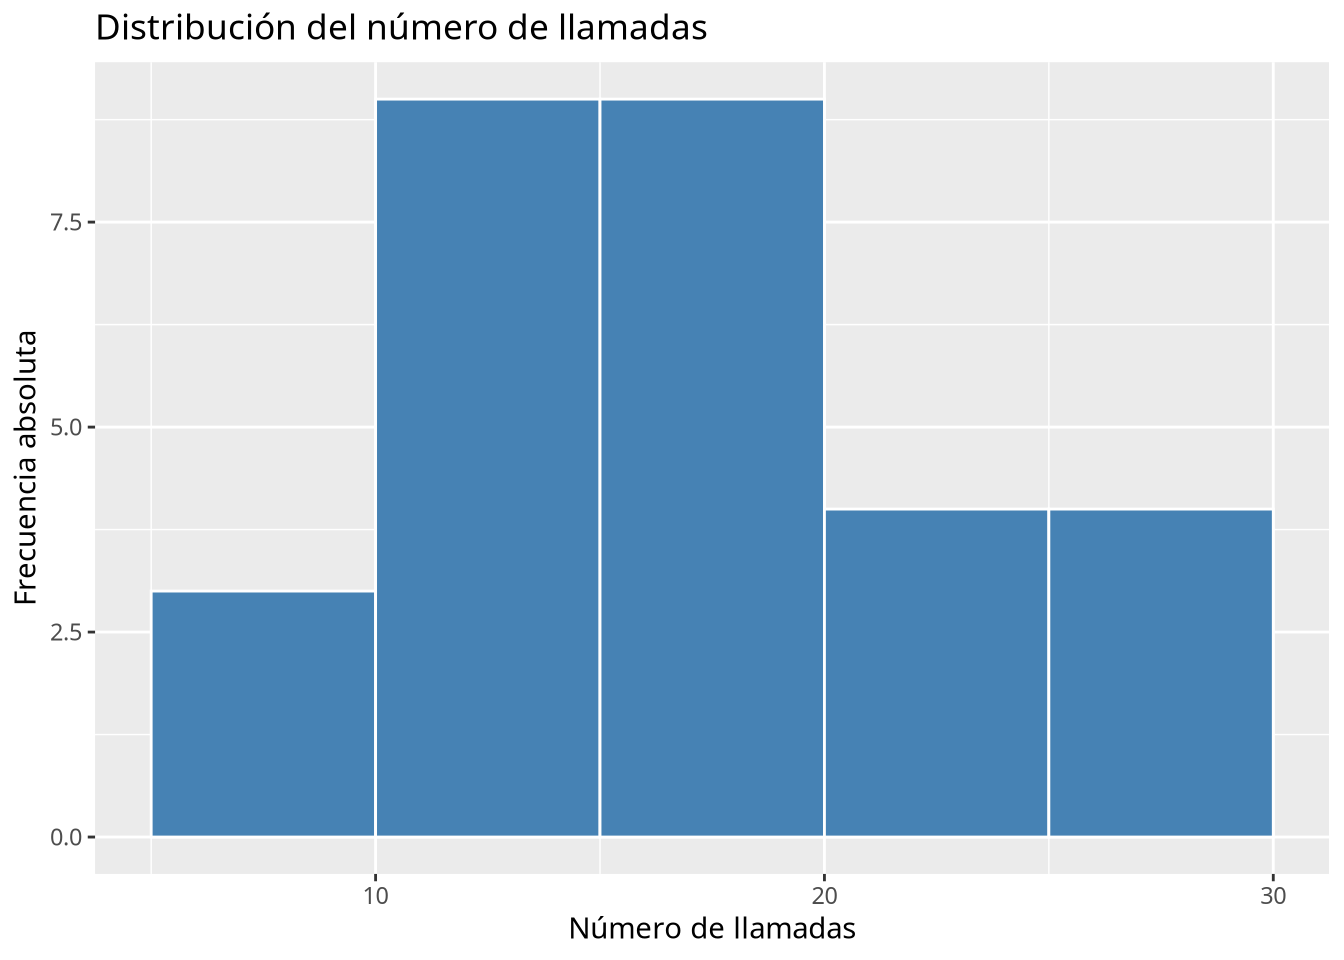
\includegraphics{./03-frecuencias-graficos_files/figure-pdf/unnamed-chunk-17-1.pdf}

}

\end{figure}

\begin{Shaded}
\begin{Highlighting}[]
\CommentTok{\# Histograma de frecuencias relativas}
\FunctionTok{ggplot}\NormalTok{(df, }\FunctionTok{aes}\NormalTok{(}\AttributeTok{x =}\NormalTok{ llamadas)) }\SpecialCharTok{+}
    \FunctionTok{geom\_histogram}\NormalTok{(}\FunctionTok{aes}\NormalTok{(}\AttributeTok{y =}\NormalTok{ (..count..)}\SpecialCharTok{/}\FunctionTok{sum}\NormalTok{(..count..)), }\AttributeTok{breaks =} \FunctionTok{seq}\NormalTok{(}\DecValTok{5}\NormalTok{, }\DecValTok{30}\NormalTok{, }\DecValTok{5}\NormalTok{), }\AttributeTok{fill =} \StringTok{"steelblue"}\NormalTok{, }\AttributeTok{col =} \StringTok{"white"}\NormalTok{) }\SpecialCharTok{+}
    \FunctionTok{labs}\NormalTok{(}\AttributeTok{title =} \StringTok{"Distribución del número de llamadas"}\NormalTok{, }\AttributeTok{x =} \StringTok{"Número de llamadas"}\NormalTok{, }\AttributeTok{y =} \StringTok{"Frecuencia relativa"}\NormalTok{)}
\end{Highlighting}
\end{Shaded}

\begin{figure}[H]

{\centering 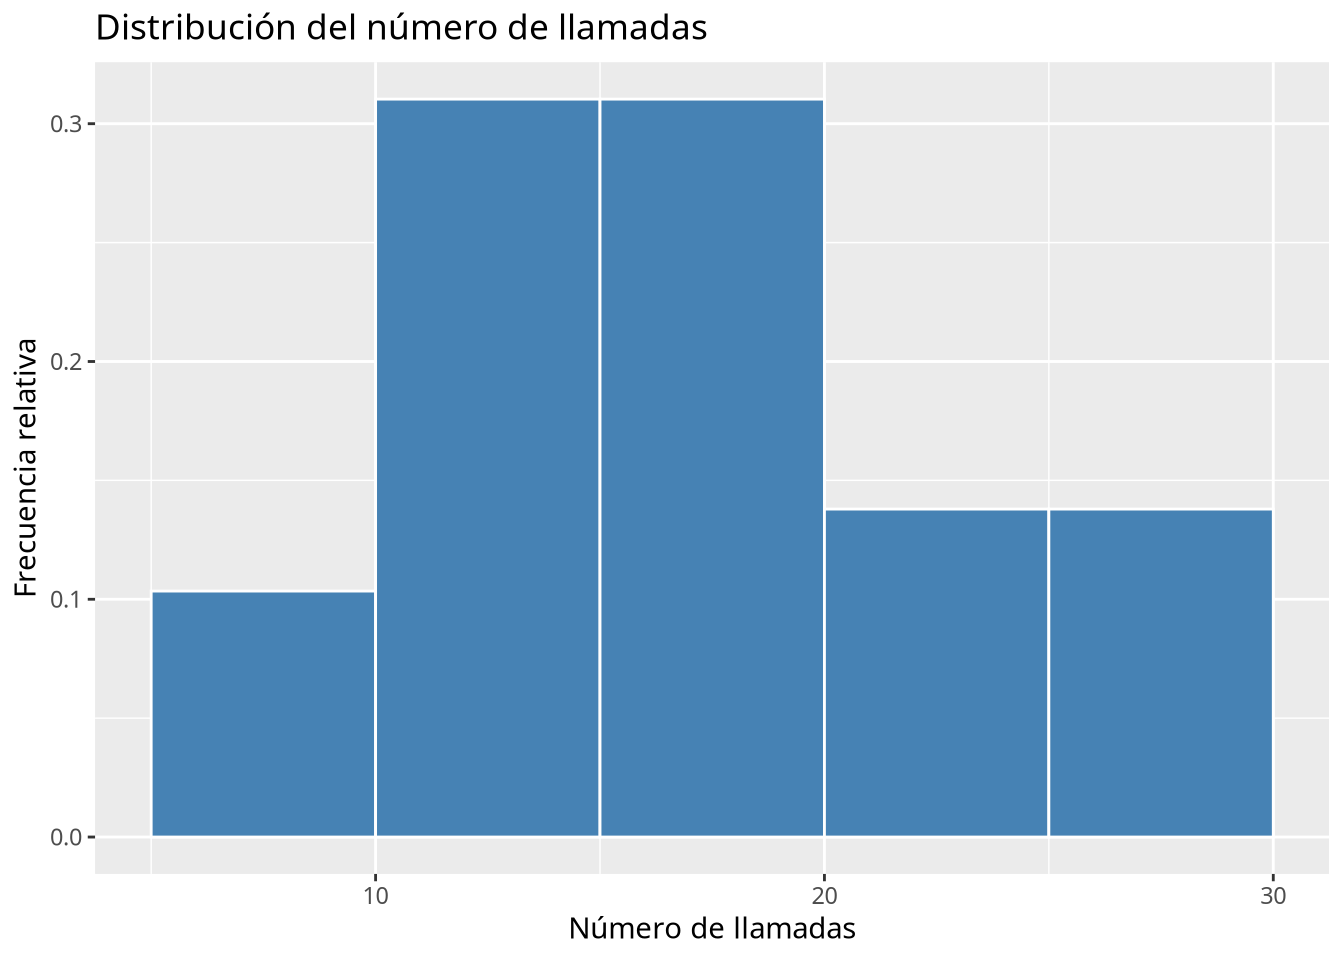
\includegraphics{./03-frecuencias-graficos_files/figure-pdf/unnamed-chunk-17-2.pdf}

}

\end{figure}

\begin{Shaded}
\begin{Highlighting}[]
\CommentTok{\# Histograma de frecuencias acumuladas}
\FunctionTok{ggplot}\NormalTok{(df, }\FunctionTok{aes}\NormalTok{(}\AttributeTok{x =}\NormalTok{ llamadas)) }\SpecialCharTok{+}
    \FunctionTok{geom\_histogram}\NormalTok{(}\FunctionTok{aes}\NormalTok{(}\AttributeTok{y =} \FunctionTok{cumsum}\NormalTok{(..count..)), }\AttributeTok{breaks =} \FunctionTok{seq}\NormalTok{(}\DecValTok{5}\NormalTok{, }\DecValTok{30}\NormalTok{, }\DecValTok{5}\NormalTok{), }\AttributeTok{fill =} \StringTok{"steelblue"}\NormalTok{, }\AttributeTok{col =} \StringTok{"white"}\NormalTok{) }\SpecialCharTok{+}
    \FunctionTok{labs}\NormalTok{(}\AttributeTok{title =} \StringTok{"Distribución acumulada del número de llamadas"}\NormalTok{, }\AttributeTok{x =} \StringTok{"Número de llamadas"}\NormalTok{, }\AttributeTok{y =} \StringTok{"Frecuencia absoluta acumulada"}\NormalTok{)}
\end{Highlighting}
\end{Shaded}

\begin{figure}[H]

{\centering 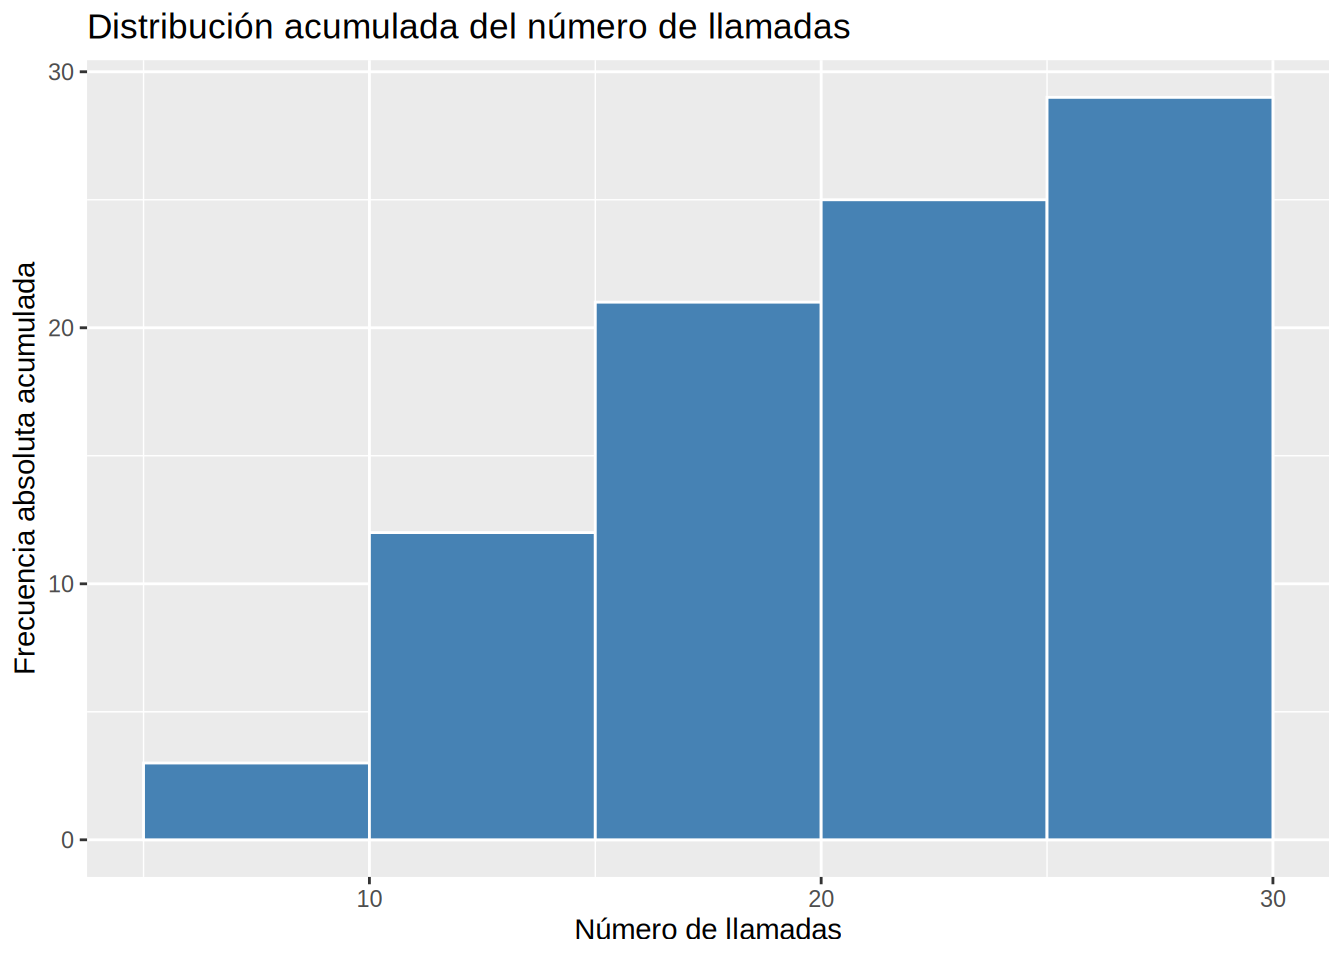
\includegraphics{./03-frecuencias-graficos_files/figure-pdf/unnamed-chunk-17-3.pdf}

}

\end{figure}

\begin{Shaded}
\begin{Highlighting}[]
\CommentTok{\# Histograma de frecuencias relativas acumuladas}
\FunctionTok{ggplot}\NormalTok{(df, }\FunctionTok{aes}\NormalTok{(}\AttributeTok{x =}\NormalTok{ llamadas)) }\SpecialCharTok{+}
    \FunctionTok{geom\_histogram}\NormalTok{(}\FunctionTok{aes}\NormalTok{(}\AttributeTok{y =} \FunctionTok{cumsum}\NormalTok{(..count..)}\SpecialCharTok{/}\FunctionTok{sum}\NormalTok{(..count..)),  }\AttributeTok{breaks =} \FunctionTok{seq}\NormalTok{(}\DecValTok{5}\NormalTok{, }\DecValTok{30}\NormalTok{, }\DecValTok{5}\NormalTok{), }\AttributeTok{fill =} \StringTok{"steelblue"}\NormalTok{, }\AttributeTok{col =} \StringTok{"white"}\NormalTok{) }\SpecialCharTok{+}
    \FunctionTok{labs}\NormalTok{(}\AttributeTok{title =} \StringTok{"Distribución acumulada del número de llamadas"}\NormalTok{, }\AttributeTok{x =} \StringTok{"Número de llamadas"}\NormalTok{, }\AttributeTok{y =} \StringTok{"Frecuencia relativa acumulada"}\NormalTok{)}
\end{Highlighting}
\end{Shaded}

\begin{figure}[H]

{\centering 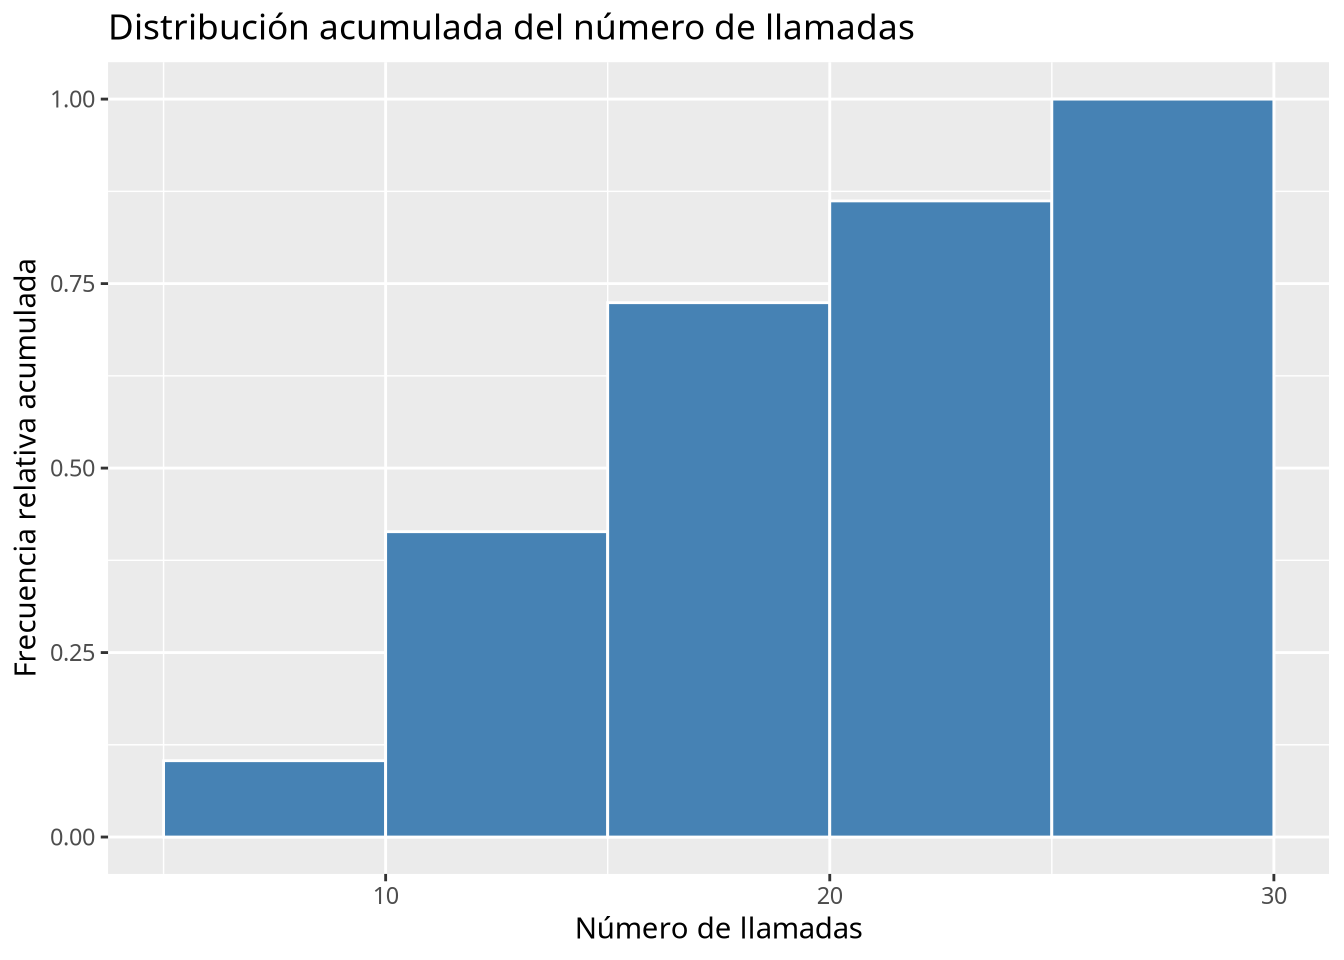
\includegraphics{./03-frecuencias-graficos_files/figure-pdf/unnamed-chunk-17-4.pdf}

}

\end{figure}

\end{tcolorbox}

\begin{enumerate}
\def\labelenumi{\alph{enumi}.}
\setcounter{enumi}{4}
\tightlist
\item
  Dibujar el polígono de frecuencias relativas acumuladas (ojiva).
\end{enumerate}

\begin{tcolorbox}[enhanced jigsaw, rightrule=.15mm, toptitle=1mm, colbacktitle=quarto-callout-tip-color!10!white, titlerule=0mm, colback=white, leftrule=.75mm, bottomtitle=1mm, colframe=quarto-callout-tip-color-frame, breakable, title=\textcolor{quarto-callout-tip-color}{\faLightbulb}\hspace{0.5em}{Solución 1}, arc=.35mm, coltitle=black, opacityback=0, bottomrule=.15mm, opacitybacktitle=0.6, left=2mm, toprule=.15mm]

Para dibujar la ojiva se puede usar la función
\href{https://www.rdocumentation.org/packages/graphics/versions/3.6.2/topics/plot}{\texttt{plot}}
del paquete \texttt{graphics}.

\begin{Shaded}
\begin{Highlighting}[]
\CommentTok{\# Ojiva}
\NormalTok{cortes }\OtherTok{=} \FunctionTok{seq}\NormalTok{(}\DecValTok{5}\NormalTok{, }\DecValTok{30}\NormalTok{, }\DecValTok{5}\NormalTok{)}
\NormalTok{ni }\OtherTok{\textless{}{-}} \FunctionTok{table}\NormalTok{(}\FunctionTok{cut}\NormalTok{(df}\SpecialCharTok{$}\NormalTok{llamadas, }\AttributeTok{breaks =}\NormalTok{ cortes))}
\NormalTok{Fi }\OtherTok{\textless{}{-}} \FunctionTok{c}\NormalTok{(}\DecValTok{0}\NormalTok{, }\FunctionTok{cumsum}\NormalTok{(ni)}\SpecialCharTok{/}\FunctionTok{sum}\NormalTok{(ni))}
\FunctionTok{plot}\NormalTok{(cortes, Fi, }\AttributeTok{type =} \StringTok{"l"}\NormalTok{, }\AttributeTok{col =} \StringTok{"steelblue"}\NormalTok{, }\AttributeTok{main =} \StringTok{"Distribución acumulada del número de llamadas"}\NormalTok{, }\AttributeTok{xlab =} \StringTok{"Número de llamadas"}\NormalTok{, }\AttributeTok{ylab =} \StringTok{"Frecuencia relativa acumulada"}\NormalTok{)}
\end{Highlighting}
\end{Shaded}

\begin{figure}[H]

{\centering 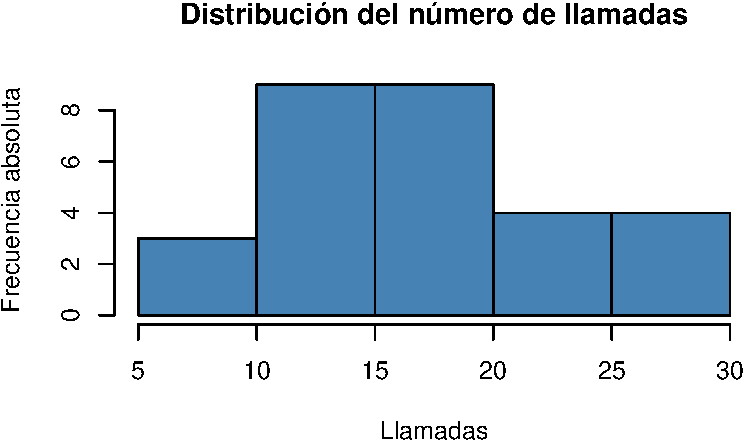
\includegraphics{./03-frecuencias-graficos_files/figure-pdf/unnamed-chunk-18-1.pdf}

}

\end{figure}

\end{tcolorbox}

\begin{tcolorbox}[enhanced jigsaw, rightrule=.15mm, toptitle=1mm, colbacktitle=quarto-callout-tip-color!10!white, titlerule=0mm, colback=white, leftrule=.75mm, bottomtitle=1mm, colframe=quarto-callout-tip-color-frame, breakable, title=\textcolor{quarto-callout-tip-color}{\faLightbulb}\hspace{0.5em}{Solución 2}, arc=.35mm, coltitle=black, opacityback=0, bottomrule=.15mm, opacitybacktitle=0.6, left=2mm, toprule=.15mm]

Otra alternativa es usar la función la función
\href{https://aprendeconalf.es/manual-r/07-graficos.html\#histogramas}{\texttt{geom\_line}}
del paquete \texttt{ggplot2}.

\begin{Shaded}
\begin{Highlighting}[]
\FunctionTok{library}\NormalTok{(ggplot2)}
\CommentTok{\# Ojiva}
\NormalTok{cortes }\OtherTok{\textless{}{-}} \FunctionTok{seq}\NormalTok{(}\DecValTok{5}\NormalTok{, }\DecValTok{30}\NormalTok{, }\DecValTok{5}\NormalTok{)}
\NormalTok{tabla\_frec }\OtherTok{\textless{}{-}} \FunctionTok{mutate}\NormalTok{(df, }\AttributeTok{llamadas\_int =} \FunctionTok{cut}\NormalTok{(df}\SpecialCharTok{$}\NormalTok{llamadas, }\AttributeTok{breaks =}\NormalTok{ cortes)) }\SpecialCharTok{\%\textgreater{}\%} 
    \FunctionTok{count}\NormalTok{(llamadas\_int) }\SpecialCharTok{\%\textgreater{}\%}
    \FunctionTok{mutate}\NormalTok{(}\AttributeTok{cortes =}\NormalTok{ cortes[}\SpecialCharTok{{-}}\DecValTok{1}\NormalTok{], }\AttributeTok{Fi =} \FunctionTok{cumsum}\NormalTok{(n)}\SpecialCharTok{/}\FunctionTok{sum}\NormalTok{(n)) }\SpecialCharTok{\%\textgreater{}\%}
    \FunctionTok{select}\NormalTok{(cortes, Fi) }
\NormalTok{tabla\_frec }\OtherTok{\textless{}{-}} \FunctionTok{rbind}\NormalTok{(}\FunctionTok{data.frame}\NormalTok{(}\AttributeTok{cortes =}\NormalTok{ cortes[}\DecValTok{1}\NormalTok{], }\AttributeTok{Fi =} \DecValTok{0}\NormalTok{), tabla\_frec)}
\FunctionTok{ggplot}\NormalTok{(tabla\_frec, }\FunctionTok{aes}\NormalTok{(}\AttributeTok{x =}\NormalTok{ cortes , }\AttributeTok{y =}\NormalTok{ Fi)) }\SpecialCharTok{+}
    \FunctionTok{geom\_line}\NormalTok{(}\AttributeTok{col =} \StringTok{"steelblue"}\NormalTok{) }\SpecialCharTok{+}
    \FunctionTok{labs}\NormalTok{(}\AttributeTok{title =} \StringTok{"Distribución del número de llamadas"}\NormalTok{, }\AttributeTok{x =} \StringTok{"Número de llamadas"}\NormalTok{, }\AttributeTok{y =} \StringTok{"Frecuencia relativa acumulada"}\NormalTok{)}
\end{Highlighting}
\end{Shaded}

\begin{figure}[H]

{\centering 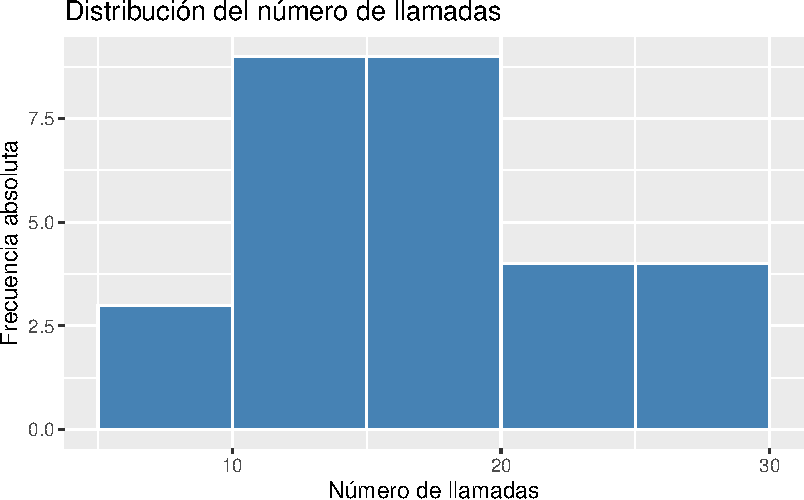
\includegraphics{./03-frecuencias-graficos_files/figure-pdf/unnamed-chunk-19-1.pdf}

}

\end{figure}

\end{tcolorbox}

\end{exercise}

\leavevmode\vadjust pre{\hypertarget{exr-3}{}}%
\begin{exercise}[]\label{exr-3}

Los grupos sanguíneos de una muestra de 30 personas son:

\begin{longtable}[]{@{}
  >{\centering\arraybackslash}p{(\columnwidth - 0\tabcolsep) * \real{1.0000}}@{}}
\toprule()
\endhead
A, B, B, A, AB, 0, 0, A, B, B, A, A, A, A, AB, A, A, A, B, 0, B, B, B,
A, A, A, 0, A, AB, 0 \\
\bottomrule()
\end{longtable}

\begin{enumerate}
\def\labelenumi{\alph{enumi}.}
\tightlist
\item
  Crear un conjunto de datos con la variable \texttt{grupo\_sanguíneo}.
\end{enumerate}

\begin{tcolorbox}[enhanced jigsaw, rightrule=.15mm, toptitle=1mm, colbacktitle=quarto-callout-tip-color!10!white, titlerule=0mm, colback=white, leftrule=.75mm, bottomtitle=1mm, colframe=quarto-callout-tip-color-frame, breakable, title=\textcolor{quarto-callout-tip-color}{\faLightbulb}\hspace{0.5em}{Solución}, arc=.35mm, coltitle=black, opacityback=0, bottomrule=.15mm, opacitybacktitle=0.6, left=2mm, toprule=.15mm]

\begin{Shaded}
\begin{Highlighting}[]
\NormalTok{df }\OtherTok{\textless{}{-}} \FunctionTok{data.frame}\NormalTok{(}\AttributeTok{grupo\_sanguineo =} \FunctionTok{c}\NormalTok{(}\StringTok{"A"}\NormalTok{, }\StringTok{"B"}\NormalTok{, }\StringTok{"B"}\NormalTok{, }\StringTok{"A"}\NormalTok{, }\StringTok{"AB"}\NormalTok{, }\StringTok{"0"}\NormalTok{, }\StringTok{"0"}\NormalTok{, }\StringTok{"A"}\NormalTok{, }\StringTok{"B"}\NormalTok{, }\StringTok{"B"}\NormalTok{, }\StringTok{"A"}\NormalTok{, }\StringTok{"A"}\NormalTok{, }\StringTok{"A"}\NormalTok{, }\StringTok{"A"}\NormalTok{, }\StringTok{"AB"}\NormalTok{, }\StringTok{"A"}\NormalTok{, }\StringTok{"A"}\NormalTok{, }\StringTok{"A"}\NormalTok{, }\StringTok{"B"}\NormalTok{, }\StringTok{"0"}\NormalTok{, }\StringTok{"B"}\NormalTok{, }\StringTok{"B"}\NormalTok{, }\StringTok{"B"}\NormalTok{, }\StringTok{"A"}\NormalTok{, }\StringTok{"A"}\NormalTok{, }\StringTok{"A"}\NormalTok{, }\StringTok{"0"}\NormalTok{, }\StringTok{"A"}\NormalTok{, }\StringTok{"AB"}\NormalTok{, }\StringTok{"0"}\NormalTok{))}
\end{Highlighting}
\end{Shaded}

\end{tcolorbox}

\begin{enumerate}
\def\labelenumi{\alph{enumi}.}
\setcounter{enumi}{1}
\tightlist
\item
  Construir la tabla de frecuencias.
\end{enumerate}

\begin{tcolorbox}[enhanced jigsaw, rightrule=.15mm, toptitle=1mm, colbacktitle=quarto-callout-tip-color!10!white, titlerule=0mm, colback=white, leftrule=.75mm, bottomtitle=1mm, colframe=quarto-callout-tip-color-frame, breakable, title=\textcolor{quarto-callout-tip-color}{\faLightbulb}\hspace{0.5em}{Solución 1}, arc=.35mm, coltitle=black, opacityback=0, bottomrule=.15mm, opacitybacktitle=0.6, left=2mm, toprule=.15mm]

Para obtener las frecuencias absolutas se puede usar la función
\href{https://www.rdocumentation.org/packages/base/versions/3.6.2/topics/table}{\texttt{table}},
y para las frecuencias relativas la función
\href{https://www.rdocumentation.org/packages/base/versions/3.6.2/topics/prop.table}{\texttt{prop.table}}
ambas del paquete base de R.

\begin{Shaded}
\begin{Highlighting}[]
\CommentTok{\# Frecuencias absolutas.}
\NormalTok{ni }\OtherTok{\textless{}{-}} \FunctionTok{table}\NormalTok{(df}\SpecialCharTok{$}\NormalTok{grupo\_sanguineo)}
\CommentTok{\# Frecuencias relativas}
\NormalTok{fi }\OtherTok{\textless{}{-}} \FunctionTok{prop.table}\NormalTok{(ni)}
\NormalTok{tabla\_frec }\OtherTok{\textless{}{-}} \FunctionTok{cbind}\NormalTok{(ni, fi)}
\NormalTok{tabla\_frec}
\end{Highlighting}
\end{Shaded}

\begin{verbatim}
   ni        fi
0   5 0.1666667
A  14 0.4666667
AB  3 0.1000000
B   8 0.2666667
\end{verbatim}

\end{tcolorbox}

\begin{tcolorbox}[enhanced jigsaw, rightrule=.15mm, toptitle=1mm, colbacktitle=quarto-callout-tip-color!10!white, titlerule=0mm, colback=white, leftrule=.75mm, bottomtitle=1mm, colframe=quarto-callout-tip-color-frame, breakable, title=\textcolor{quarto-callout-tip-color}{\faLightbulb}\hspace{0.5em}{Solución 2}, arc=.35mm, coltitle=black, opacityback=0, bottomrule=.15mm, opacitybacktitle=0.6, left=2mm, toprule=.15mm]

Otra alternativa es usar la fución
\href{https://aprendeconalf.es/manual-r/06-preprocesamiento.html\#conteo-del-n\%C3\%BAmero-de-observaciones}{\texttt{count}}
del paquete \texttt{dplyr}.

\begin{Shaded}
\begin{Highlighting}[]
\FunctionTok{library}\NormalTok{(dplyr)}
\FunctionTok{library}\NormalTok{(knitr)}
\FunctionTok{library}\NormalTok{(kableExtra)}
\FunctionTok{count}\NormalTok{(df, grupo\_sanguineo) }\SpecialCharTok{\%\textgreater{}\%} 
    \FunctionTok{mutate}\NormalTok{(}\AttributeTok{fi =}\NormalTok{ n}\SpecialCharTok{/}\FunctionTok{sum}\NormalTok{(n)) }\SpecialCharTok{\%\textgreater{}\%}
    \FunctionTok{kable}\NormalTok{() }
\end{Highlighting}
\end{Shaded}

\begin{tabular}{l|r|r}
\hline
grupo\_sanguineo & n & fi\\
\hline
0 & 5 & 0.1666667\\
\hline
A & 14 & 0.4666667\\
\hline
AB & 3 & 0.1000000\\
\hline
B & 8 & 0.2666667\\
\hline
\end{tabular}

\begin{Shaded}
\begin{Highlighting}[]
    \CommentTok{\#\%\textgreater{}\%}
    \CommentTok{\#kable\_styling(bootstrap\_options = "hover", full\_width = F)}
\end{Highlighting}
\end{Shaded}

\end{tcolorbox}

\begin{enumerate}
\def\labelenumi{\alph{enumi}.}
\setcounter{enumi}{2}
\tightlist
\item
  Dibujar el diagrama de sectores.
\end{enumerate}

\begin{tcolorbox}[enhanced jigsaw, rightrule=.15mm, toptitle=1mm, colbacktitle=quarto-callout-tip-color!10!white, titlerule=0mm, colback=white, leftrule=.75mm, bottomtitle=1mm, colframe=quarto-callout-tip-color-frame, breakable, title=\textcolor{quarto-callout-tip-color}{\faLightbulb}\hspace{0.5em}{Solución 1}, arc=.35mm, coltitle=black, opacityback=0, bottomrule=.15mm, opacitybacktitle=0.6, left=2mm, toprule=.15mm]

Para dibujar el diagrama de sectores se puede usar la función
\href{https://www.rdocumentation.org/packages/graphics/versions/3.6.2/topics/pie}{\texttt{pie}}
del paquete \texttt{graphics}.

\begin{Shaded}
\begin{Highlighting}[]
\CommentTok{\# Diagrama de sectores}
\FunctionTok{pie}\NormalTok{(ni, }\AttributeTok{col =} \DecValTok{1}\SpecialCharTok{:}\FunctionTok{length}\NormalTok{(ni), }\AttributeTok{main =} \StringTok{"Distribución de los grupos sanguíneos"}\NormalTok{)}
\end{Highlighting}
\end{Shaded}

\begin{figure}[H]

{\centering 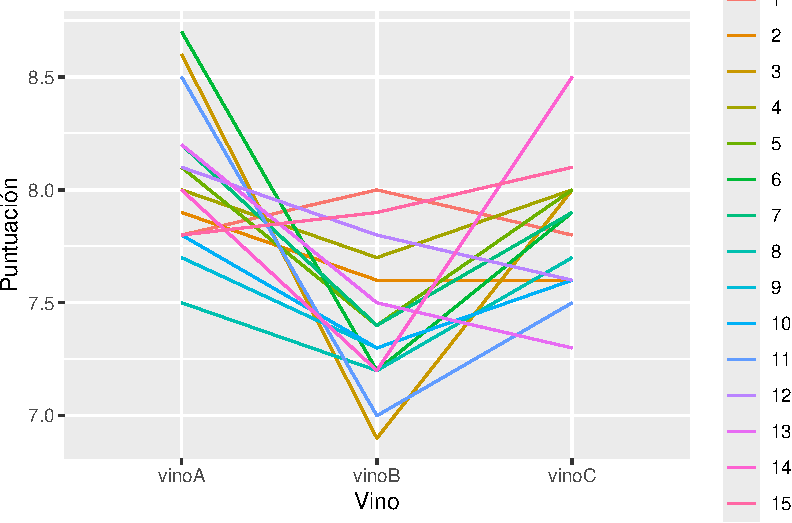
\includegraphics{./03-frecuencias-graficos_files/figure-pdf/unnamed-chunk-23-1.pdf}

}

\end{figure}

\end{tcolorbox}

\begin{tcolorbox}[enhanced jigsaw, rightrule=.15mm, toptitle=1mm, colbacktitle=quarto-callout-tip-color!10!white, titlerule=0mm, colback=white, leftrule=.75mm, bottomtitle=1mm, colframe=quarto-callout-tip-color-frame, breakable, title=\textcolor{quarto-callout-tip-color}{\faLightbulb}\hspace{0.5em}{Solución 2}, arc=.35mm, coltitle=black, opacityback=0, bottomrule=.15mm, opacitybacktitle=0.6, left=2mm, toprule=.15mm]

Otra alternativa es usar las fuciones
\href{https://aprendeconalf.es/manual-r/07-graficos.html\#diagrama-de-sectores}{\texttt{geom\_bar}}
y \texttt{coor\_polar} del paquete \texttt{ggplot2}.

\begin{Shaded}
\begin{Highlighting}[]
\FunctionTok{ggplot}\NormalTok{(df, }\FunctionTok{aes}\NormalTok{(}\AttributeTok{x =} \StringTok{""}\NormalTok{, }\AttributeTok{fill =}\NormalTok{ grupo\_sanguineo)) }\SpecialCharTok{+}
    \CommentTok{\# Añadir la capa de las barras.}
    \FunctionTok{geom\_bar}\NormalTok{() }\SpecialCharTok{+}
    \CommentTok{\# Añadir el sistema de coordenadas polares}
    \FunctionTok{coord\_polar}\NormalTok{(}\AttributeTok{theta =} \StringTok{"y"}\NormalTok{) }\SpecialCharTok{+}
    \FunctionTok{labs}\NormalTok{(}\AttributeTok{title =} \StringTok{"Distribución de los grupos sanguíneos"}\NormalTok{)}
\end{Highlighting}
\end{Shaded}

\begin{figure}[H]

{\centering 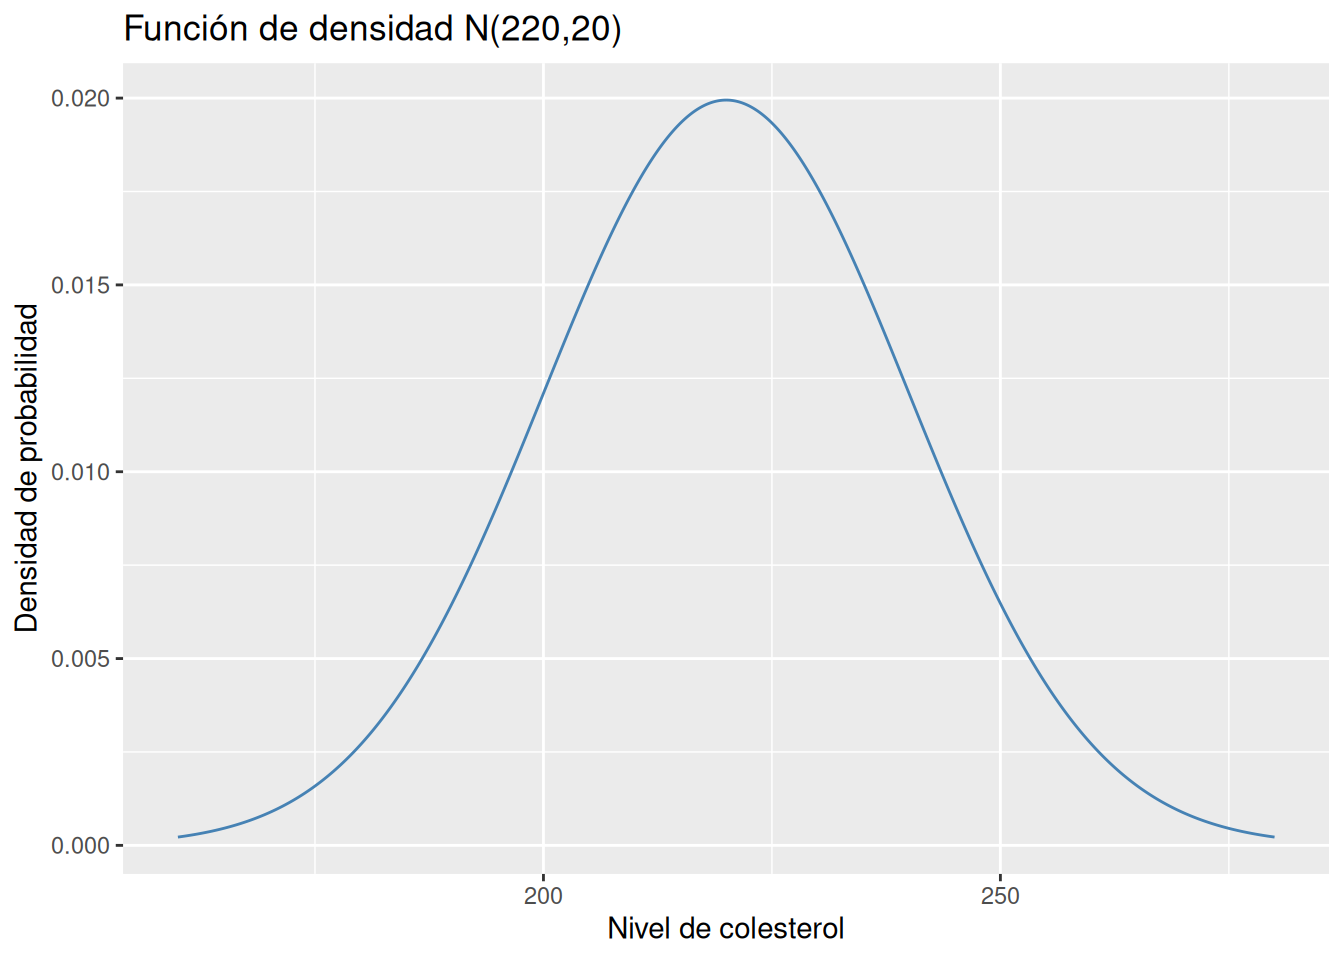
\includegraphics{./03-frecuencias-graficos_files/figure-pdf/unnamed-chunk-24-1.pdf}

}

\end{figure}

\end{tcolorbox}

\end{exercise}

\leavevmode\vadjust pre{\hypertarget{exr-4}{}}%
\begin{exercise}[]\label{exr-4}

En un estudio de población se tomó una muestra de 27 personas, y se les
preguntó por su edad y estado civil, obteniendo los siguientes
resultados:

\begin{longtable}[]{@{}ll@{}}
\toprule()
Estado civil & Edad \\
\midrule()
\endhead
Soltero & 31, 45, 35, 65, 21, 38, 62, 22, 31 \\
Casado & 62, 39, 62, 59, 21, 62 \\
Viudo & 80, 68, 65, 40, 78, 69, 75 \\
Divorciado & 31, 65, 59, 49, 65 \\
\bottomrule()
\end{longtable}

\begin{enumerate}
\def\labelenumi{\alph{enumi}.}
\tightlist
\item
  Crear un conjunto de datos con la variables \texttt{estado\_civil} y
  \texttt{edad}.
\end{enumerate}

\begin{tcolorbox}[enhanced jigsaw, rightrule=.15mm, toptitle=1mm, colbacktitle=quarto-callout-tip-color!10!white, titlerule=0mm, colback=white, leftrule=.75mm, bottomtitle=1mm, colframe=quarto-callout-tip-color-frame, breakable, title=\textcolor{quarto-callout-tip-color}{\faLightbulb}\hspace{0.5em}{Solución}, arc=.35mm, coltitle=black, opacityback=0, bottomrule=.15mm, opacitybacktitle=0.6, left=2mm, toprule=.15mm]

\begin{Shaded}
\begin{Highlighting}[]
\NormalTok{df }\OtherTok{\textless{}{-}} \FunctionTok{data.frame}\NormalTok{(}
    \AttributeTok{edad =} \FunctionTok{c}\NormalTok{(}\DecValTok{31}\NormalTok{, }\DecValTok{45}\NormalTok{, }\DecValTok{35}\NormalTok{, }\DecValTok{65}\NormalTok{, }\DecValTok{21}\NormalTok{, }\DecValTok{38}\NormalTok{, }\DecValTok{62}\NormalTok{, }\DecValTok{22}\NormalTok{, }\DecValTok{31}\NormalTok{, }\DecValTok{62}\NormalTok{, }\DecValTok{39}\NormalTok{, }\DecValTok{62}\NormalTok{, }\DecValTok{59}\NormalTok{, }\DecValTok{21}\NormalTok{, }\DecValTok{62}\NormalTok{, }\DecValTok{80}\NormalTok{, }\DecValTok{68}\NormalTok{, }\DecValTok{65}\NormalTok{, }\DecValTok{40}\NormalTok{, }\DecValTok{78}\NormalTok{, }\DecValTok{69}\NormalTok{, }\DecValTok{75}\NormalTok{, }\DecValTok{31}\NormalTok{, }\DecValTok{65}\NormalTok{, }\DecValTok{59}\NormalTok{, }\DecValTok{49}\NormalTok{, }\DecValTok{65}\NormalTok{), }
    \AttributeTok{estado\_civil =} \FunctionTok{rep}\NormalTok{(}\FunctionTok{c}\NormalTok{(}\StringTok{"Soltero"}\NormalTok{, }\StringTok{"Casado"}\NormalTok{, }\StringTok{"Viudo"}\NormalTok{, }\StringTok{"Divorciado"}\NormalTok{), }\FunctionTok{c}\NormalTok{(}\DecValTok{9}\NormalTok{, }\DecValTok{6}\NormalTok{, }\DecValTok{7}\NormalTok{, }\DecValTok{5}\NormalTok{)))}
\end{Highlighting}
\end{Shaded}

\end{tcolorbox}

\begin{enumerate}
\def\labelenumi{\alph{enumi}.}
\setcounter{enumi}{1}
\tightlist
\item
  Construir la tabla de frecuencias de la variable \texttt{edad} para
  cada categoría de la variable \texttt{estado\_civil}.
\end{enumerate}

\begin{tcolorbox}[enhanced jigsaw, rightrule=.15mm, toptitle=1mm, colbacktitle=quarto-callout-tip-color!10!white, titlerule=0mm, colback=white, leftrule=.75mm, bottomtitle=1mm, colframe=quarto-callout-tip-color-frame, breakable, title=\textcolor{quarto-callout-tip-color}{\faLightbulb}\hspace{0.5em}{Solución}, arc=.35mm, coltitle=black, opacityback=0, bottomrule=.15mm, opacitybacktitle=0.6, left=2mm, toprule=.15mm]

Para dividir la muestra en grupos se puede usar la función
\href{https://aprendeconalf.es/manual-r/06-preprocesamiento.html\#res\%C3\%BAmenes-por-grupos}{\texttt{group-by}}
del paquete \texttt{dplyr}.

\begin{Shaded}
\begin{Highlighting}[]
\FunctionTok{library}\NormalTok{(dplyr)}
\FunctionTok{library}\NormalTok{(knitr)}
\FunctionTok{library}\NormalTok{(kableExtra)}
\FunctionTok{mutate}\NormalTok{(df, }\AttributeTok{edad\_int =} \FunctionTok{cut}\NormalTok{(edad, }\AttributeTok{breaks =} \FunctionTok{seq}\NormalTok{(}\DecValTok{20}\NormalTok{, }\DecValTok{80}\NormalTok{, }\DecValTok{10}\NormalTok{))) }\SpecialCharTok{\%\textgreater{}\%}
    \FunctionTok{group\_by}\NormalTok{(estado\_civil) }\SpecialCharTok{\%\textgreater{}\%}
    \FunctionTok{count}\NormalTok{(edad\_int) }\SpecialCharTok{\%\textgreater{}\%} 
    \FunctionTok{mutate}\NormalTok{(}\AttributeTok{fi =}\NormalTok{ n}\SpecialCharTok{/}\FunctionTok{sum}\NormalTok{(n), }\AttributeTok{Ni =} \FunctionTok{cumsum}\NormalTok{(n), }\AttributeTok{Fi =} \FunctionTok{cumsum}\NormalTok{(n)}\SpecialCharTok{/}\FunctionTok{sum}\NormalTok{(n)) }\SpecialCharTok{\%\textgreater{}\%}
    \FunctionTok{kable}\NormalTok{() }
\end{Highlighting}
\end{Shaded}

\begin{tabular}{l|l|r|r|r|r}
\hline
estado\_civil & edad\_int & n & fi & Ni & Fi\\
\hline
Casado & (20,30] & 1 & 0.1666667 & 1 & 0.1666667\\
\hline
Casado & (30,40] & 1 & 0.1666667 & 2 & 0.3333333\\
\hline
Casado & (50,60] & 1 & 0.1666667 & 3 & 0.5000000\\
\hline
Casado & (60,70] & 3 & 0.5000000 & 6 & 1.0000000\\
\hline
Divorciado & (30,40] & 1 & 0.2000000 & 1 & 0.2000000\\
\hline
Divorciado & (40,50] & 1 & 0.2000000 & 2 & 0.4000000\\
\hline
Divorciado & (50,60] & 1 & 0.2000000 & 3 & 0.6000000\\
\hline
Divorciado & (60,70] & 2 & 0.4000000 & 5 & 1.0000000\\
\hline
Soltero & (20,30] & 2 & 0.2222222 & 2 & 0.2222222\\
\hline
Soltero & (30,40] & 4 & 0.4444444 & 6 & 0.6666667\\
\hline
Soltero & (40,50] & 1 & 0.1111111 & 7 & 0.7777778\\
\hline
Soltero & (60,70] & 2 & 0.2222222 & 9 & 1.0000000\\
\hline
Viudo & (30,40] & 1 & 0.1428571 & 1 & 0.1428571\\
\hline
Viudo & (60,70] & 3 & 0.4285714 & 4 & 0.5714286\\
\hline
Viudo & (70,80] & 3 & 0.4285714 & 7 & 1.0000000\\
\hline
\end{tabular}

\begin{Shaded}
\begin{Highlighting}[]
    \CommentTok{\#\%\textgreater{}\%}
    \CommentTok{\#kable\_styling(bootstrap\_options = "hover", full\_width = F)}
\end{Highlighting}
\end{Shaded}

\end{tcolorbox}

\begin{enumerate}
\def\labelenumi{\alph{enumi}.}
\setcounter{enumi}{2}
\tightlist
\item
  Dibujar los diagramas de cajas de la edad según el estado civil.
  ¿Existen datos atípicos? ¿En qué grupo hay mayor dispersión?
\end{enumerate}

\begin{tcolorbox}[enhanced jigsaw, rightrule=.15mm, toptitle=1mm, colbacktitle=quarto-callout-tip-color!10!white, titlerule=0mm, colback=white, leftrule=.75mm, bottomtitle=1mm, colframe=quarto-callout-tip-color-frame, breakable, title=\textcolor{quarto-callout-tip-color}{\faLightbulb}\hspace{0.5em}{Solución}, arc=.35mm, coltitle=black, opacityback=0, bottomrule=.15mm, opacitybacktitle=0.6, left=2mm, toprule=.15mm]

\begin{Shaded}
\begin{Highlighting}[]
\FunctionTok{library}\NormalTok{(ggplot2)}
\FunctionTok{ggplot}\NormalTok{(df, }\FunctionTok{aes}\NormalTok{(}\AttributeTok{x =}\NormalTok{ edad, }\AttributeTok{fill =}\NormalTok{ estado\_civil)) }\SpecialCharTok{+}
    \FunctionTok{geom\_boxplot}\NormalTok{()}
\end{Highlighting}
\end{Shaded}

\begin{figure}[H]

{\centering 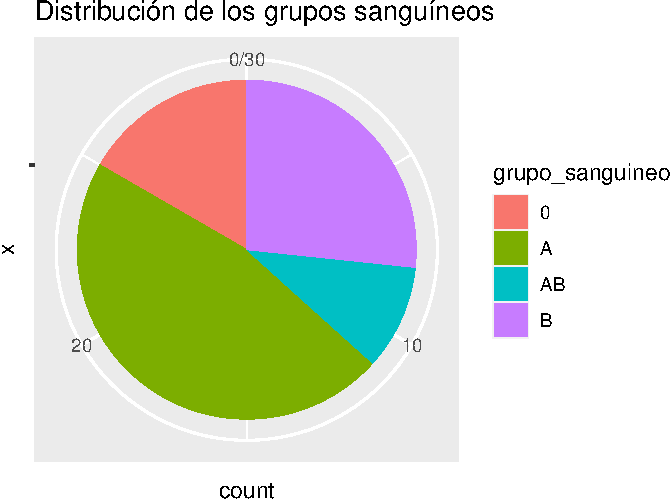
\includegraphics{./03-frecuencias-graficos_files/figure-pdf/unnamed-chunk-27-1.pdf}

}

\end{figure}

\end{tcolorbox}

\begin{enumerate}
\def\labelenumi{\alph{enumi}.}
\setcounter{enumi}{3}
\tightlist
\item
  Dibujar los histogramas de la edad según el estado civil.
\end{enumerate}

\begin{tcolorbox}[enhanced jigsaw, rightrule=.15mm, toptitle=1mm, colbacktitle=quarto-callout-tip-color!10!white, titlerule=0mm, colback=white, leftrule=.75mm, bottomtitle=1mm, colframe=quarto-callout-tip-color-frame, breakable, title=\textcolor{quarto-callout-tip-color}{\faLightbulb}\hspace{0.5em}{Solución}, arc=.35mm, coltitle=black, opacityback=0, bottomrule=.15mm, opacitybacktitle=0.6, left=2mm, toprule=.15mm]

\begin{Shaded}
\begin{Highlighting}[]
\FunctionTok{ggplot}\NormalTok{(df, }\FunctionTok{aes}\NormalTok{(}\AttributeTok{x =}\NormalTok{ edad, }\AttributeTok{fill =}\NormalTok{ estado\_civil)) }\SpecialCharTok{+}
    \FunctionTok{geom\_histogram}\NormalTok{(}\AttributeTok{breaks =} \FunctionTok{seq}\NormalTok{(}\DecValTok{20}\NormalTok{, }\DecValTok{80}\NormalTok{, }\DecValTok{10}\NormalTok{), }\AttributeTok{position =} \StringTok{"identity"}\NormalTok{, }\AttributeTok{alpha=}\FloatTok{0.4}\NormalTok{)}
\end{Highlighting}
\end{Shaded}

\begin{figure}[H]

{\centering 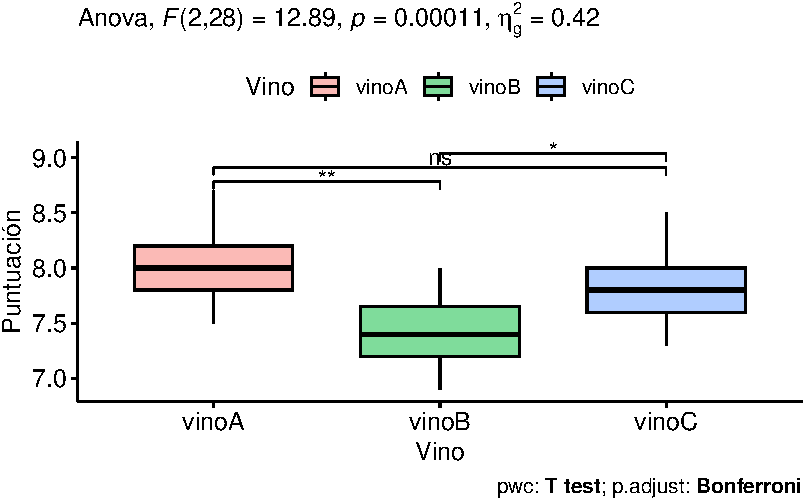
\includegraphics{./03-frecuencias-graficos_files/figure-pdf/unnamed-chunk-28-1.pdf}

}

\end{figure}

Para dibujar cada histograma por separado se puede usar la función
\href{https://aprendeconalf.es/manual-r/07-graficos.html\#facetas}{\texttt{facet\_wrap}}
o \texttt{facet\_grid} del paquete \texttt{ggplot2}.

\begin{Shaded}
\begin{Highlighting}[]
\FunctionTok{ggplot}\NormalTok{(df, }\FunctionTok{aes}\NormalTok{(}\AttributeTok{x =}\NormalTok{ edad, }\AttributeTok{fill =}\NormalTok{ estado\_civil)) }\SpecialCharTok{+}
    \FunctionTok{geom\_histogram}\NormalTok{(}\AttributeTok{breaks =} \FunctionTok{seq}\NormalTok{(}\DecValTok{20}\NormalTok{, }\DecValTok{80}\NormalTok{, }\DecValTok{10}\NormalTok{)) }\SpecialCharTok{+}
    \CommentTok{\# Añadir la faceta del estado civil}
    \FunctionTok{facet\_grid}\NormalTok{(}\AttributeTok{rows =} \FunctionTok{vars}\NormalTok{(estado\_civil))}
\end{Highlighting}
\end{Shaded}

\begin{figure}[H]

{\centering 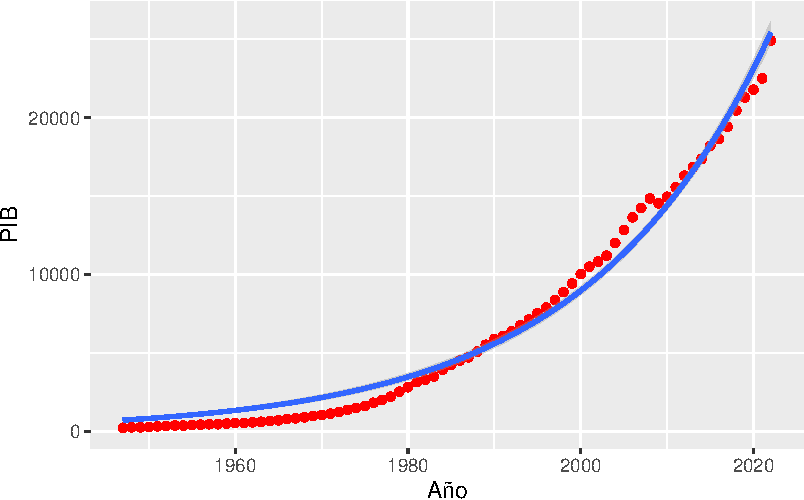
\includegraphics{./03-frecuencias-graficos_files/figure-pdf/unnamed-chunk-29-1.pdf}

}

\end{figure}

\end{tcolorbox}

\end{exercise}

\hypertarget{ejercicios-propuestos-1}{%
\section{Ejercicios propuestos}\label{ejercicios-propuestos-1}}

El conjunto de datos \href{datos/neonatos.csv}{neonatos} contiene
información sobre una muestra de 320 recién nacidos en un hospital
durante un año que cumplieron el tiempo normal de gestación.

\begin{enumerate}
\def\labelenumi{\alph{enumi}.}
\item
  Construir la tabla de frecuencias de la puntuación Apgar al minuto de
  nacer. Si se considera que una puntuación Apgar de 3 o menos indica
  que el neonato está deprimido, ¿qué porcentaje de niños está deprimido
  en la muestra?
\item
  Comparar las distribuciones de frecuencias de las puntuaciones Apgar
  al minuto de nacer según si la madre es mayor o menor de 20 años. ¿En
  qué grupo hay más neonatos deprimidos?
\item
  Construir la tabla de frecuencias para el peso de los neonatos,
  agrupando en clases de amplitud \(0.5\) desde el \(2\) hasta el
  \(4.5\). ¿En qué intervalo de peso hay más neonatos?
\item
  Comparar la distribución de frecuencias relativas del peso de los
  neonatos según si la madre fuma o no. Si se considera como peso bajo
  un peso menor de \(2.5\) kg, ¿En qué grupo hay un mayor porcentaje de
  niños con peso bajo?
\item
  Si en los recién nacidos se considera como peso bajo un peso menor de
  \(2.5\) kg, calcular la prevalencia del bajo peso de recién nacidos en
  el grupo de madres fumadoras y en el de no fumadoras.
\item
  Construir el diagrama de barras de la puntuación Apgar al minuto. ¿Qué
  puntuación Apgar es la más frecuente?
\item
  Construir el diagrama de frecuencias relativas acumuladas de la
  puntuación Apgar al minuto. ¿Por debajo de que puntuación estarán la
  mitad de los niños?
\item
  Comparar mediante diagramas de barras de frecuencias relativas las
  distribuciones de las puntuaciones Apgar al minuto según si la madre
  ha fumado o no durante el embarazo. ¿Qué se puede concluir?
\item
  Construir el histograma de pesos, agrupando en clases de amplitud
  \(0.5\) desde el \(2\) hasta el \(4.5\). ¿En qué intervalo de peso hay
  más niños?
\item
  Comparar la distribución de frecuencias relativas del peso de los
  neonatos según si la madre fuma o no. ¿En qué grupo se aprecia menor
  peso de los niños de la muestra?
\item
  Comparar la distribución de frecuencias relativas del peso de los
  neonatos según si la madre fumaba o no antes del embarazo. ¿Qué se
  puede concluir?
\item
  Construir el diagrama de caja y bigotes del peso. ¿Entre qué valores
  se considera que el peso de un neonato es normal? ¿Existen datos
  atípicos?
\item
  Comparar el diagrama de cajas y bigotes del peso, según si la madre
  fumó o no durante el embarazo y si era mayor o no de 20 años. ¿En qué
  grupo el peso tiene más dispersión central? ¿En qué grupo pesan menos
  los niños de la muestra?
\item
  Comparar el diagrama de cajas de la puntuación Apgar al minuto y a los
  cinco minutos. ¿En qué variable hay más dispersión central?
\end{enumerate}



\end{document}
